%-------------------------------------------------------------------------------
% This file provides a skeleton ATLAS note.
% \pdfinclusioncopyfonts=1
% This command may be needed in order to get \ell in PDF plots to appear. Found in
% https://tex.stackexchange.com/questions/322010/pdflatex-glyph-undefined-symbols-disappear-from-included-pdf
%-------------------------------------------------------------------------------
% Specify where ATLAS LaTeX style files can be found.
\newcommand*{\ATLASLATEXPATH}{latex/}
% Use this variant if the files are in a central location, e.g. $HOME/texmf.
% \newcommand*{\ATLASLATEXPATH}{}
%-------------------------------------------------------------------------------
\documentclass[NOTE, atlasdraft=true, texlive=2016, UKenglish]{\ATLASLATEXPATH atlasdoc}
% The language of the document must be set: usually UKenglish or USenglish.
% british and american also work!
% Commonly used options:
%  atlasdraft=true|false This document is an ATLAS draft.
%  texlive=YYYY          Specify TeX Live version (2016 is default).
%  coverpage             Create ATLAS draft cover page for collaboration circulation.
%                        See atlas-draft-cover.tex for a list of variables that should be defined.
%  cernpreprint          Create front page for a CERN preprint.
%                        See atlas-preprint-cover.tex for a list of variables that should be defined.
%  NOTE                  The document is an ATLAS note (draft).
%  PAPER                 The document is an ATLAS paper (draft).
%  CONF                  The document is a CONF note (draft).
%  PUB                   The document is a PUB note (draft).
%  BOOK                  The document is of book form, like an LOI or TDR (draft)
%  txfonts=true|false    Use txfonts rather than the default newtx
%  paper=a4|letter       Set paper size to A4 (default) or letter.

%-------------------------------------------------------------------------------
% Extra packages:
\usepackage[subfigure]{\ATLASLATEXPATH atlaspackage}
% Commonly used options:
%  biblatex=true|false   Use biblatex (default) or bibtex for the bibliography.
%  backend=bibtex        Use the bibtex backend rather than biber.
%  subfigure|subfig|subcaption  to use one of these packages for figures in figures.
%  minimal               Minimal set of packages.
%  default               Standard set of packages.
%  full                  Full set of packages.
\usepackage{multirow}
\usepackage{pdflscape}
%-------------------------------------------------------------------------------
% Style file with biblatex options for ATLAS documents.
\usepackage{\ATLASLATEXPATH atlasbiblatex}

% Package for creating list of authors and contributors to the analysis.
\usepackage{\ATLASLATEXPATH atlascontribute}

% Useful macros
\usepackage{\ATLASLATEXPATH atlasphysics}
% See doc/atlas_physics.pdf for a list of the defined symbols.
% Default options are:
%   true:  journal, misc, particle, unit, xref
%   false: BSM, heppparticle, hepprocess, hion, jetetmiss, math, process, other, texmf
% See the package for details on the options.

% Files with references for use with biblatex.
% Note that biber gives an error if it finds empty bib files.
\addbibresource{ANA-EXOT-2019-32-INT1.bib}
\addbibresource{bib/ATLAS.bib}
\addbibresource{bib/CMS.bib}
\addbibresource{bib/ConfNotes.bib}
\addbibresource{bib/PubNotes.bib}

% Paths for figures - do not forget the / at the end of the directory name.
\graphicspath{{logos/}{figures/}}

% Add you own definitions here (file ANA-EXOT-2019-32-INT1-defs.sty).
\usepackage{ANA-EXOT-2019-32-INT1-defs}

%-------------------------------------------------------------------------------
% Generic document information
%-------------------------------------------------------------------------------

% Title, abstract and document
%-------------------------------------------------------------------------------
% This file contains the title, author and abstract.
% It also contains all relevant document numbers used for an ATLAS note.
%-------------------------------------------------------------------------------

% Title
\AtlasTitle{Search for new phenomena in dijet events using quark gluon tagging based on track multiplicty}

% Draft version:
% Should be 1.0 for the first circulation, and 2.0 for the second circulation.
% If given, adds draft version on front page, a 'DRAFT' box on top of each other page, 
% and line numbers.
% Comment or remove in final version.
\AtlasVersion{0.1}

% Abstract - % directly after { is important for correct indentation
\AtlasAbstract{%
A search for new resonance decays producing a pair of jets is
performed using 139~fb$^{-1}$ of ATLAS $pp$ collision data recorded from the
Large Hadron Collider operating at $\sqrt{s} = 13$~TeV. 
To increase the sensitivity to observe new resonances preferentially
decaying to one or more gluons, a gluon-tag method based on the number
of associated particle tracks is employed.
No significant excess of events above a smoothly falling dijet
background distribution is observed.
The results are used to set cross-section upper limits at the 95\%
confidence level for signal-gluon and double-gluon tagged jets
originating from new resonance decays.
Model-dependent string scale lower limits are set on string resonances
which predominantly decay to a gluon and quark, and mass lower limits
on a massive colour-singlet scalar particle decaying exclusively to
two gluons.  
}

% Author - this does not work with revtex (add it after \begin{document})
%\author{The ATLAS Collaboration}

% Authors and list of contributors to the analysis
% \AtlasAuthorContributor also adds the name to the author list
% Include package latex/atlascontribute to use this
% Use authblk package if there are multiple authors, which is included by latex/atlascontribute
% \usepackage{authblk}
% Use the following 3 lines to have all institutes on one line
\makeatletter
\renewcommand\AB@affilsepx{, \protect\Affilfont}
\makeatother
% \renewcommand\Authands{, } % avoid ``. and'' for last author
% \renewcommand\Affilfont{\itshape\small} % affiliation formatting
% Alphabetising

\AtlasAuthorContributor{Iain~Bertram}{a}{Contact, supervising Rybacki, q/g tagging optimisation of selection, statistical framework.}
\AtlasAuthorContributor{Jyoti~Biswal}{b}{BG estimation, systematics.}
\AtlasAuthorContributor{Shih-Chieh~Hsu}{d}{Supervising students, checking analysis flow, data MC comparison.}
\AtlasAuthorContributor{Doug~Gingrich}{b,c}{Supervising Lyons.}
\AtlasAuthorContributor{Jack~Lindon}{b}{ Data Fitting, Statistical Studies.}
\AtlasAuthorContributor{Fairhurst~Lyons}{b}{BG estimation, systematics.}
\AtlasAuthorContributor{Ben~Nachman}{e}{CP uncertainties; supervising Rybacki.}
\AtlasAuthorContributor{Nishu~Nishu}{b}{Analysis advice.}
\AtlasAuthorContributor{Katherine~Rybacki}{a}{q/g tagging systematics, sample production.}
\AtlasAuthorContributor{Shu~Li}{g}{ Supervising students}
\AtlasAuthorContributor{Wanyun~Su}{g}{Checking analysis flow, data MC comparison.}
\AtlasAuthorContributor{Changxu~Wei}{h}{Checking analysis flow, data MC comparison.}
\AtlasAuthorContributor{Dengfeng~Zhang}{b}{Ntuple Creation, Optimisation of Data Selection}
\AtlasAuthorContributor{Yan~Zhou}{h}{Checking analysis flow, data MC comparison.}
% \AtlasContributor{.}
% \author[a]{Iain Bertram}
% \author[a]{Second Author}
% \author[b]{Third Author}
\affil[a]{Lancaster}
\affil[b]{Alberta}
\affil[c]{TRIUMF}
\affil[d]{Seattle Washington}
\affil[e]{Berkeley LBNL}
\affil[f]{Shanghai}
\affil[g]{TDLI}
\affil[h]{Beijing Tsinghau}

% If a special author list should be indicated via a link use the following code:
% Include the two lines below if you do not use atlasstyle:
% \usepackage[marginal,hang]{footmisc}
% \setlength{\footnotemargin}{0.5em}
% Use the following lines in all cases:
% \usepackage{authblk}
% \author{The ATLAS Collaboration%
% \thanks{The full author list can be found at:\newline
%   \url{https://atlas.web.cern.ch/Atlas/PUBNOTES/ATL-PHYS-PUB-2016-007/authorlist.pdf}}
% }

% ATLAS reference code, to help ATLAS members to locate the paper
\AtlasRefCode{ANA-EXOT-2019-32}

% ATLAS note number. Can be an COM, INT, PUB or CONF note
\AtlasNote{ANA-EXOT-2019-32-INT1}

% Author and title for the PDF file
\hypersetup{pdftitle={ATLAS document},pdfauthor={The ATLAS Collaboration}}

%-------------------------------------------------------------------------------
% Content
%-------------------------------------------------------------------------------
\begin{document}

\maketitle

\tableofcontents

% List of contributors - print here or after the Bibliography.
%\PrintAtlasContribute{0.30}
%\clearpage

%-------------------------------------------------------------------------------
\section{Introduction}
\label{sec:intro}
Searches for anomalous dijet events can be sensitive to a large set of models for Beyond the Standard Model (BSM) physics.
This includes new particles arising from additional broken gauge groups,
excitations of Standard Model particles (for instance Kaluza-Klein excitations in models involving extra dimensions),
interactions between dark matter and the Standard Model, and models of quark compositeness.
If any new particles can be produced at hadron colliders then they must couple to Standard Model (SM) partons.
This coupling means the new particles can decay to jets, often dominantly.
The total dijet production rates for such signals can be large even at substantial fractions of the
total hadron collision energy, allowing searches to begin to probe these energy regimes with relatively little data.

For these reasons, searches in dijet events are often amongst of the first searches done when a hadron
collider reaches a new energy frontier\footnote{See Ref.~\cite{Harris:2011bh} for a review of the history
of these searches from UA1 and UA2 to the LHC Run 1.}.  Increases in collision centre-of-mass energy, \s , 
dramatically improves the reach of searches for potential high-mass signals. 
Increases in the integrated luminosity of the data samples results in much smaller improvements and requires significant 
improvements in the understanding of systematic uncertainties. 

A search for new physics both in the dijet mass distribution and in the angular distributions was performed on 13~\TeV\xspace data collected in 2015 and 2016 \cite{EXOT-2016-21} with the  95\% CL lower limits on the masses given in Table~\ref{tab:Limits201516}. 
Most of the strategies and methods of the analysis are mostly unchanged with respect to the previous iterations of the analysis, which can be reviewed in great detail in the internal
notes \cite{Bauce:2226443}.


%The increase in collision center-of-mass energy \s\ from
%8 to 13~\TeV\xspace dramatically enhances parton luminosities at multi-\TeV\xspace energies
%(Fig.~\ref{fig:partonluminosity}) and thus the production rates of potential high-mass signals.


\begin{table}[!h]
	\centering
	\caption{The 95\% CL lower limits on the masses of ADD quantum black holes (\textsc{\BlackMax} event generator), \Wprime\ and \Wstar\ bosons, excited quarks, and $Z^\prime$ bosons for selected coupling values from the resonance search, as well as on the scale of contact interactions for constructive ($\eta_{\text{LL}}=-1$) and destructive ($\eta_{\text{LL}}=+1$) interference from the angular analysis. Where an additional range is listed, masses within the range are also excluded.}
	\begin{tabular}{ l c c}
		\toprule
		\multicolumn{1}{c}{Model} & \multicolumn{2}{c}{95\% CL exclusion limit} \\
		\cmidrule(r){2-3}
		&  Observed & Expected \\
		\midrule
		Quantum black hole &  8.9~TeV\xspace  & 8.9~TeV\xspace \\
		\midrule
		\Wprime  & 3.6~TeV\xspace &   3.7~TeV\xspace \\
		\midrule
		\multirow{2}{*}{\Wstar}  & 3.4~TeV\xspace  &    \multirow{2}{*}{~3.6~TeV\xspace}  \\
		&3.77~TeV -- 3.85~TeV & \\		
		\midrule
		Excited quark & 6.0~TeV\xspace  &   5.8~TeV\xspace  \\
		\midrule
		\Zprime ($g_q= 0.1$)  & 2.1~TeV\xspace & 2.1~TeV\xspace \\
		\midrule
		\Zprime ($g_q= 0.2$)  & 2.9~TeV\xspace & 3.3~TeV\xspace \\
		\midrule                                               
		Contact interaction ($\eta_{\text{LL}}= -1$) & 21.8~TeV\xspace\phantom{.} & 28.3~TeV\xspace\phantom{.} \\
		\midrule
		\multirow{2}{*}{Contact interaction ($\eta_{\text{LL}}= +1$)}  & 13.1~TeV\xspace\phantom{.} & \multirow{2}{*}{15.0~TeV\xspace\phantom{.}} \\
		& 17.4~TeV\xspace\ -- 29.5~TeV\xspace & \\
		\bottomrule
	\end{tabular}
	\label{tab:Limits201516}
\end{table}


If the resonant data sample can be separated  based on the type of  parton that initiated the jets the 
sensitivity of the search should be significantly increased. The fraction of events as a function of 
the dijet mass from QCD  simulated with a  \textsc{Pythia~8.186}~\cite{pythia8} and the leading-order NNPDF2.3~\cite{Ball:2012cx} parton distribution functions (PDFs) is shown in Fig.~\ref{fig:quarkgluonfraction}. 
This suggests that tagging quark and gluon jets should be able to improve the sensitivity of searches for new particles. 
ATLAS has 
published a study \cite{ATL-PHYS-PUB-2017-009} showing that jets can be tagged as quark or gluon jets 
based on the number of charged particles with transverse momentum (\pt ) above 500\,MeV. 
In this note we present the analysis for the whole combined 2015 and 2016 13~\TeV\xspace dataset using quark 
and gluon tagging  based on charged-particle constituent multiplicity.

\begin{figure}[htb]
 \centering
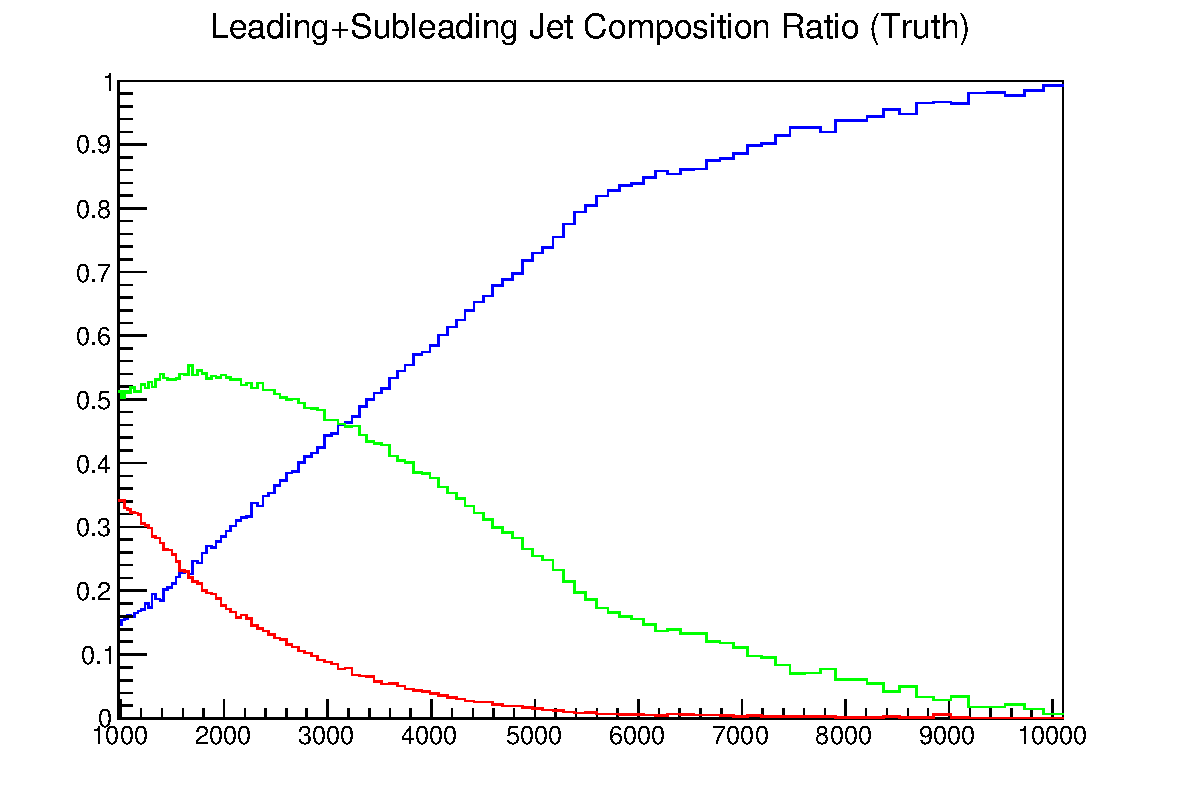
\includegraphics[width=0.75\textwidth]{figures/introduction/truthCompositionRatio.pdf}
\caption{The fraction of dijet events that are initiated by quark-quark events (blue), quark-gluon 
events (green) and gluon-gluon events (red) in simulated data.  \label{fig:quarkgluonfraction}}
\end{figure}

\subsection{Overview of the analysis}
\label{sec:overview}

First, we demonstrate using toy MCs that tagging quark and gluon jets can, in principle, make significant 
improvements to the sensitivity of the resonance search.

The subsequent analysis of the data will follow previously used in the analysis of the 2015 and 2016 data 
\cite{EXOT-2016-21,Bauce:2226443}. This is reproduced here for convinience. 


We analyze dijet events using the dijet invariant mass \mjj\  (described in Section \ref{sec:observables}).

The initial analysis steps are

\begin{enumerate}
\item Unprescaled single-jet triggers are used to collect events containing
highly energetic jets (Section~\ref{sec:trigger})
\item High-\pT\xspace jets are reconstructed, identified, and calibrated according to recommendations, with techniques
prepared in tandem between the analysis team and the
JetEtMiss group (Section~\ref{sec:jet_reconstruction}).
\item After calibration, bulk processing of the data, and production of a standardized xAOD derivation, events are selected with very similar kinematic 
criteria as in previous dijet searches (Section~\ref{sec:event_selection}). The data and Monte Carlo used are described in
Section~\ref{sec:benchmark_signals}. Prior to the availability of the data in the final
analysis, analyzers closely monitor the on-line and offline data preparation and
quality efforts for advance warning of problems.%(Appendix~\ref{app:dqchecks}).
\item When the data are available for inclusion in the analysis, the jet kinematics, calibration performance, 
and quality are monitored at the analysis level with a set of studies (Sections~\ref{sec:jet_reconstruction}).
\end{enumerate}


Statistical tests are employed in a
\textit{search phase}, described in Section~\ref{sec:background_estimation_search}, to determine whether the 
data are compatible with a background expectation. 
A localized excess (i.e. a bump) on the smooth \mjj\  distribution
is the target of the resonance analysis.
The background model is derived from a fit to the \mjj\ distribution.
A single localized excess will not bias
this fit in a significant way. The
search phase in the angular method is designed for non-resonant
signals, deriving the background model from Monte Carlo (MC)
simulation. 
The background estimation strategy is described in Section~\ref{sec:background_estimation}.
A description of systematic uncertainties can be found in 
Sections~\ref{sec:systematics_backgrounds} and \ref{sec:systematics_signal}. 
In case either method observes a significant excess, additional tests in the search phase
are detailed in Section~\ref{sec:cross_checks}. The results of the
search phase are shown in Section~\ref{sec:search_results}.

If no new phenomena is found, a ~\textit{limit setting phase} is used
to constrain a set of signals: 
\begin{itemize}
 \item Limits on benchmark signals:
\begin{itemize}
 \item Excited quarks - a benchmark resonant signal.
 \item Contact interactions- the standard benchmark of new, non-resonant phenomena.
 \item Limits on Quantum Black Holes (QBH).
 \item Limits on hadronically decaying \Wprime .
 \item Limits on hadronically decaying \Wstar .
 \item Limits on dark-matter inspired \Zprime\ models.
\end{itemize}
 \item Limits on Gaussian-shaped signal templates.
\end{itemize}
The techniques and tools used for the limit setting are described in
Sections~\ref{subsec:limits_mass} for the resonance analysis. The
systematic uncertainties considered on the benchmark signals are
detailed in Section~\ref{sec:systematics_signal}.
Each of the following sections clarifies what is consistent
with the previous iteration and what has been further developed.


 \subsection{Strategy for applying quark-gluon selection to the 2015 and 2016 data.}
 \label{sec:201516data}

The analysis strategy, cuts, and other details were developed and implemented in previous analyses \cite{EXOT-2016-21,Bauce:2226443}.  
The search and limit setting using quark-gluon tagging will take place after the selection criteria 
have been optimised and the expected sensitivity calculated.

When all the quality checks on the subsamples (see Section~\ref{sec:jet_reconstruction})
show physical behaviour, are smooth, and in general agreement
with the simulation we will proceed with the search.
Where appropriate we take the
JES uncertainty into account in our assessment of the agreement
between data and simulation. 
Pythia is only a LO generator
and we are probing a region where the PDF fits do not
have a lot of information so some difference in the shapes
can exist. Therefore we do not put a strict statistical measure
on the compatibility of the kinematic distributions but rather
look for any local features indicative of operational or
calibration issues or non-physical behaviour.


 
\subsection{Strategy for inclusion of new data}
\label{sec:blinding}

Essentially the same methodology will be  applied to the 2017 and 2018 data as is applied to 
the 2015 and 2016 data  (Section \ref{sec:201516data}). When all the quality checks on the 
subsamples (see Section~\ref{sec:jet_reconstruction}) show physical behaviour, are smooth, and 
in general agreement
with the simulation we will proceed with the search.
 

\clearpage
%-------------------------------------------------------------------------------

%-------------------------------------------------------------------------------
\section{Benchmark Models and Datasets}
\label{sec:benchmark_signals}
This section outlines benchmark models for both Quantum Chromodynamics (\QCD)~and for new
physics signals and is taken directly from \cite{Bauce:2226443}. These are used in the search and limit-setting phases of the
analysis and for testing the effects of potential
resonant and non-resonant signals on the search phase.
The main characteristics of resonant and non-resonant
signals are encapsulated in the models chosen:
\Hprime\ , String.
%excited quarks (\qstar{}), quantum black holes (\QBH), 
%a \Wprime\ signal with decays to quarks,
%\Zprime\ signals consist with recent recommendations from the 
%ATLAS-CMS Dark Matter Forum~\cite{Abercrombie:2015wmb},
%a \Wstar\ signal with decays to quarks,
%and non-resonant contact interactions (\CI).

Samples reconstructed with release 21.2 are used for 2015 and 2016 data as well as for Monte Carlo. EXOT2 skimmed samples, described in~\cite{ATLAS:Exot2Derivation}, are used in this analysis.

\subsection{Quantum Chromodynamics}
\label{qcdsamps}
\QCD processes from the SM are simulated at leading order (\LO)
and next-to-leading order (\NLO) in perturbative \QCD. 
%Table~\ref{tab:qcdSamps} gives the details on the \QCD~MC used.

In order to obtain a \NLO~prediction from \Pythia~events, they are reweighted to the 
predictions of NLOJET++ (\NLO~$K$-factors) and subsequently by Electroweak (EW) $\kappa$~factors. 
These $K$-factors and $\kappa$~factors are binned in \mjj\ and $\chi$; full details are given in Sec.~\ref{sec:ang_bkgd}.  The \NLO\ corrected
version of \Pythia8 is used for the statistical comparison of the 
data to the background for the angular analysis.

\QCD samples span such a large range in cross section that the
production must be split in order to obtain comparable statistical precision
across the kinematic range of interest.
The well established procedure of dividing \QCD~production according
to the leading jet \pT~and reweighting the underlying spectrum
is described in Ref.~\cite{Marshall:2016630}.  

\subsection{Resonant Models}
\subsubsection{H prime}
\label{sec:hprime}
%\subsubsection{Excited quarks}
%\label{sec:qstar}
%
%Excited quark (\qstar) production and subsequent decay to
%quarks and gluons via gauge interactions has been
%used as a common benchmark for the dijet mass resonance
%search~\cite{EXOT-2010-01,EXOT-2010-02,EXOT-2010-07,EXOT-2011-07,EXOT-2013-11,EXOT-2016-21},
%and it is described in detail in Refs~\cite{Baur:1987ga,Baur:1989kv}.
%The $qg\to$ \qstar production model~\cite{Baur:1987ga,Baur:1989kv} is used,
%with the assumption of spin 1/2 and quark-like SM coupling constants.
%The compositeness scale ($\Lambda$) is set to the \qstar~mass.
%
%The excited quark signal templates are generated for different mass values
%(Table~\ref{tab:qStarSamps}) with the \Pythia~8 event generator~\cite{pythia8},
%using the A14 tune~\cite{A14tune} and NNPDF2.3 PDF set~\cite{Carrazza:2013axa}. Both light flavor ($u$,$d$,$s$) and heavy flavor ($c$,$b$) quarks are taken into account in
%the event generation.
%After a basic selection, no duplicate events have been identified.
%All samples are fully simulated using \Geant.
%
%
%Figures~\ref{fig:signal_xsec} and~\ref{fig:acc} show the cross sections and
%acceptances as a function of the signal mass point.  
%The acceptance shown for the \qstar model for 13~\TeV~center-of-mass energies 
%uses the full resonance analysis selection (Section~\ref{sec:event_selection}).
%The interpolation between points is a straight line therefore the
%acceptance between m=1~\TeV~and m=2~\TeV~is not an accurate representation
%of what the acceptance of a m=1.5~\TeV~sample would be.  The
%interpolation is not used but drawn to help guide the eye.
%
%\begin{figure}[!htb]
%  \centering
%  \subfigure[Cross section]{ \label{fig:signal_xsec} 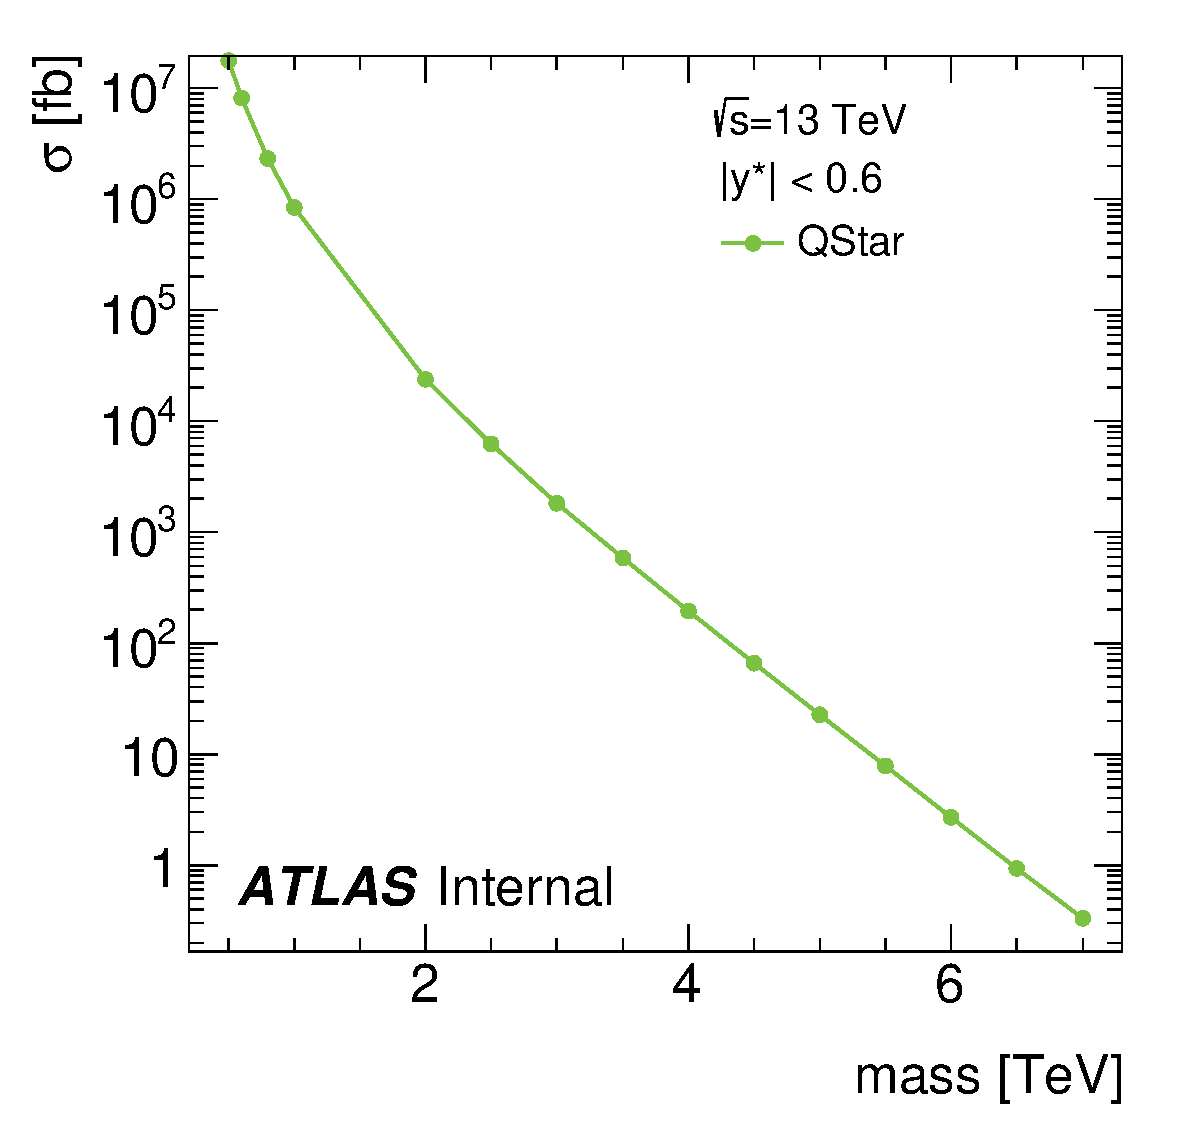
\includegraphics[width=0.48\textwidth]{figures/benchmark_signals/CrossSections_QStar_log} }
%  \subfigure[Acceptance]{ \label{fig:acc} 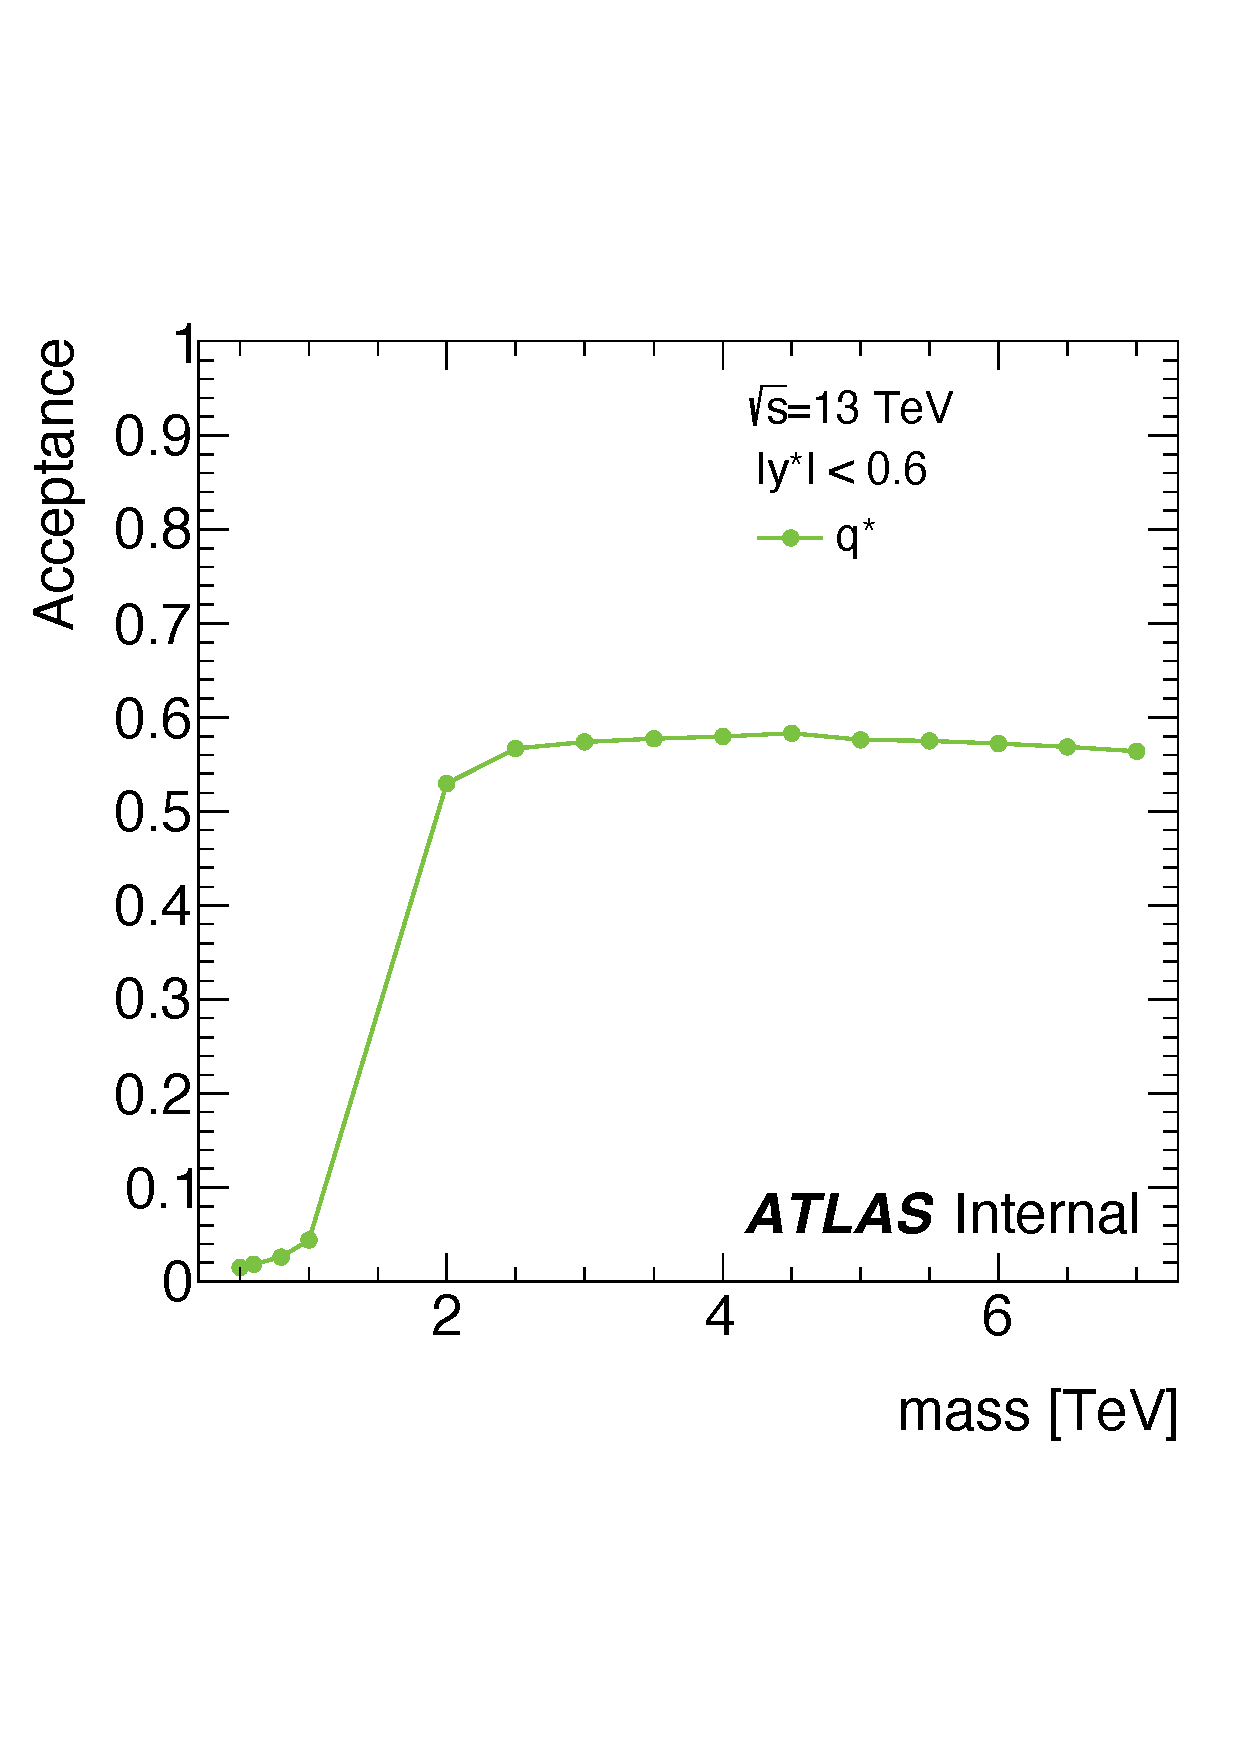
\includegraphics[width=0.48\textwidth]{figures/benchmark_signals/Acceptances_QStar} }
%  \caption{(a) Cross section and (b) acceptance for the 
%  light-flavored \qstar model for 13~\TeV~center-of-mass energies using the full resonance
%  analysis selection (Section~\ref{sec:event_selection}).}
%\end{figure}


\clearpage
\subsubsection{String}
\label{sec:string}

%\subsubsection{Quantum Black Holes}
%\label{sec:QBH}
%\todo{Do QBH decay to quarks or gluons, is there increased sensitivity or not} 
%The LHC should be able to produce QBH under the condition that the
%universe contains sufficiently large extra dimensions \cite{RandallMeade}.
%The quantum-gravity energy scale $M_{D}$ at which micro black holes are produced decreases as the number, $n$,
%of these large extra dimensions increases, allowing for lower mass scales at larger $n$.
%
%In the simplest situation, one would expect approximately isotropic decay of these micro black holes via Hawking
%radiation to a many-particle final state. This would require black holes (BH) to be produced substantially
%above their mass threshold in order to have energy for such a decay \cite{Feng:2004}. 
%However, gravitational interactions are also expected at the scale of the new interaction 
%(well below the actual thermal black hole production threshold), at which the dominant final state would be two-body ones.
%Production of these
%states is expected to begin once the $M_D$ energy threshold is reached. 
%This results in a resonance-like production of predominantly
%two-body final states, mainly jets, near $M_D$. The dijet analysis, then, is a way to search for such
%isotropic final states as probes of quantum gravitational effects.
%
%The \BlackMax~\cite{Dai:2007ki} MC generator is used to simulate quantum black holes events with $n=6$. The samples used in the analysis
%are listed in Table~\ref{tab:qbhSamps}. Cross sections and acceptances for the model are given in figures~\ref{fig:signal_xsec_blackmax} and~\ref{fig:acc_blackmax} respectively.
%
%\begin{figure}[!htb]
%  \centering
%  \subfigure[Cross section]{\label{fig:signal_xsec_blackmax} 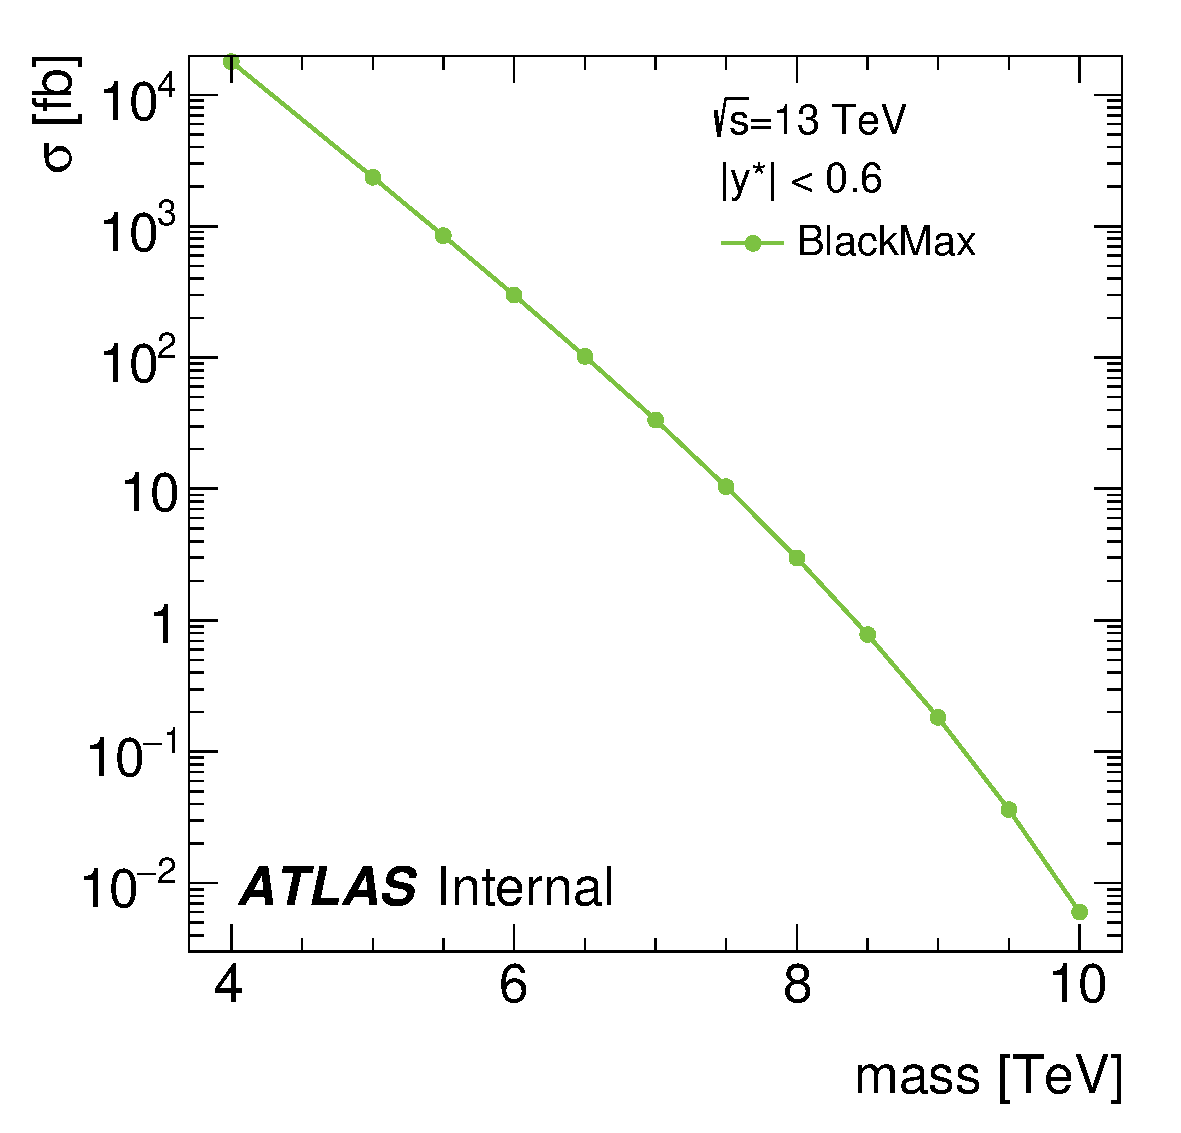
\includegraphics[width=0.48\textwidth]{figures/benchmark_signals/CrossSections_BlackMax_log}}
%  \subfigure[Acceptance]{  \label{fig:acc_blackmax}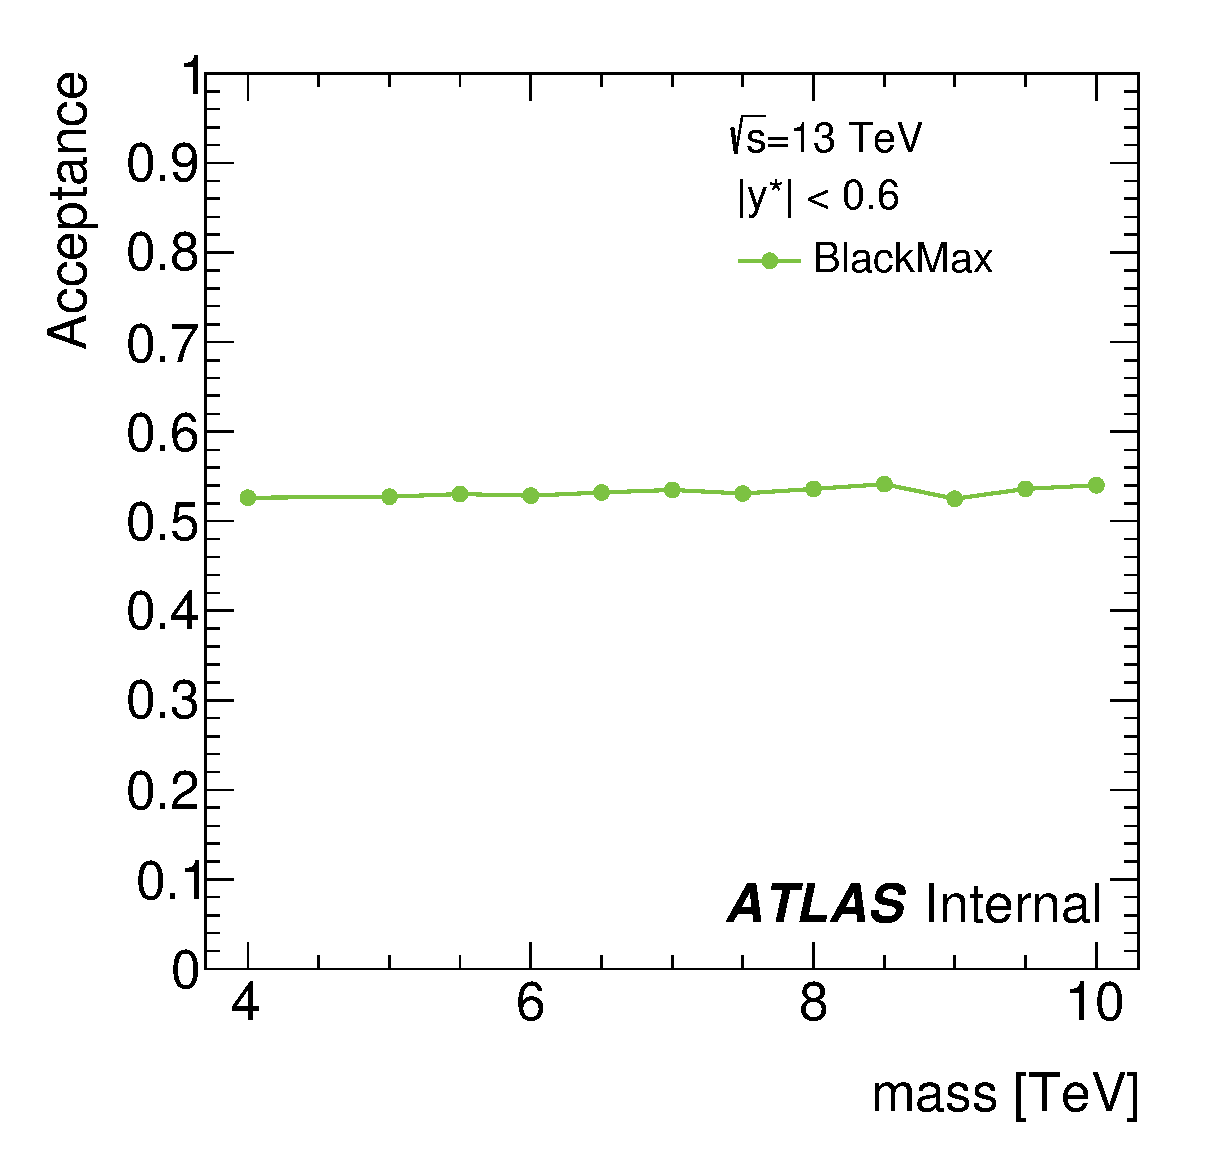
\includegraphics[width=0.48\textwidth]{figures/benchmark_signals/Acceptances_BlackMax}}
%  \caption{(a) Cross section and (b) acceptance for the 
%  \BlackMax\ model for 13~\TeV~center-of-mass energies using the full resonance
%  analysis selection (Section~\ref{sec:event_selection}).}
%
%\end{figure}
%
%
%
%\clearpage

%\subsubsection{\Zprime\ models}
%\label{sec:Zprime}
%
%Searches for dijet resonances play an important role in constraining
%possible interactions between dark matter, or a "dark sector," and the
%Standard Model. In this analysis, we consider the pure axial-vector
%leptophobic \Zprime\ model described by the ATLAS-CMS Dark Matter Forum
%Report \cite{Abercrombie:2015wmb}, in the specific scenario outlined in Ref.\cite{Chala:2015ama}, 
%where dijet searches complement mono-jet-like searches in regions of
%parameter space where the decay of the \Zprime\ to invisible particles is
%kinetically suppressed. Regions of the parameter space of this model
%remain which can be probed by dijet resonance searches but LUX, relic
%density constraints, and monojet searches cannot constrain.
%% 
%In this model, the \Zprime\ arises from a simple extension of the Standard
%Model (SM) with an additional $U(1)$ gauge symmetry and a Dirac
%fermion Dark Matter particle that has charges only under this new
%group. Assuming that some SM particles are also charged under this
%group, the \Zprime\ can mediate interactions between the SM and DM. The DM
%particle $\chi$ has a mass $m_{DM}$. The spin-1 \Zprime\ has mass \mMed.
%
%The Dark Matter Forum reports models with vector or axial-vector couplings
%between the spin-1 mediator $\Zprime$ and SM and DM fields, with the corresponding interaction Lagrangians:
%
%\begin{align}
%	\label{eq:AV}
%	\mathcal{L}_{\mathrm{vector}} &= \gq \sum_{q={u,d,s,c,b,t}}  \Zprime_{\mu} \bar{q}\gamma^{\mu}q + \gDM \Zprime_{\mu} \bar{\chiDM}\gamma^{\mu}\chiDM \\
%	\mathcal{L}_{\mathrm{axial-vector}} &= \gq \sum_{q={u,d,s,c,b,t}}  \Zprime_{\mu} \bar{q}\gamma^{\mu}\gamma^5q + \gDM \Zprime_{\mu} \bar{\chiDM}\gamma^{\mu}\gamma^5\chiDM.
%\end{align}
%
%The parameters in the model are thus
%\begin{equation}
%\left\{~\gq, 
%~ \gDM, 
%~\mDM,
%~\mMed,
%\right\} \,.
%\end{equation}
%
%where ~\gq is the coupling of the \Zprime\ mediator to quarks, ~ \gDM
%is its coupling to the Dark Matter fermion, ~\mDM is the mass
%of the Dark Matter fermion and~\mMed is the \Zprime\ mass. 
%
%The two most relevant parameters of this model in the dijet search are the coupling of the \Zprime\ to quarks
%as it drives the intrinsic width of the resonance, and the \Zprime\ mass. 
%These two parameters are scanned to obtain the signal grid used
%for the limit setting. The Dark Matter mass is fixed at 10 TeV and the coupling to DM to 1.5, with 
%a negligible effect on the resonance width. 
%% 
%The values of $\gq$ and $\mMed$ have been kept consistent with the previous published dijet result.
%The requested $\mMed$ points only go up to 3.5~TeV. This is where the resonance reaches the maximum width
%that this search is sensitive to, without incurring in significant background distortion. 
%For wider signals, it would be necessary to account for interference with the standard model.
%
%The grid of samples produced in full simulation is shown in Table~\ref{tab:ZPrimeScan}.
%
%\begin{table}[!h]
%	\centering
%		\begin{tabular}{| l |r r r r r r r r r r|}
%			\hline
%			\multicolumn{1}{|c|}{\mMed/\gev} & \multicolumn{10}{c|}{\gq} \\
%			\hline
%			1500   	       &         0.1  & 0.2 & 0.3 &  &  &  &  &  &  &  \\
%			2000           &         0.1  & 0.2 & 0.3 & 0.4  &  &  &  &  &  &  \\
%			2500           &         0.1  & 0.2 & 0.3 & 0.4 & 0.5 &  &  &  &  &  \\
%			3000           &         0.1  & 0.2 & 0.3 & 0.4 & 0.5 &  &  &  &  &  \\
%			3500           &         0.1  & 0.2 & 0.3 & 0.4 & 0.5 &  &  &  &  &  \\
%			\hline
%		\end{tabular}
%%	}
%	\caption{Parameter grid in \gq and \mMed scanned in full simulation with 25 ns configuration.}.
%	\label{tab:ZPrimeScan}
%\end{table}
% 
% The acceptances %and cross-sections 
% for the \Zprime\ samples
% are shown in Figure~\ref{fig:zprime_acc}.% and \ref{fig:zprime_xsec} respectively. 
%
% \begin{figure}[!htb]
%   \centering
%   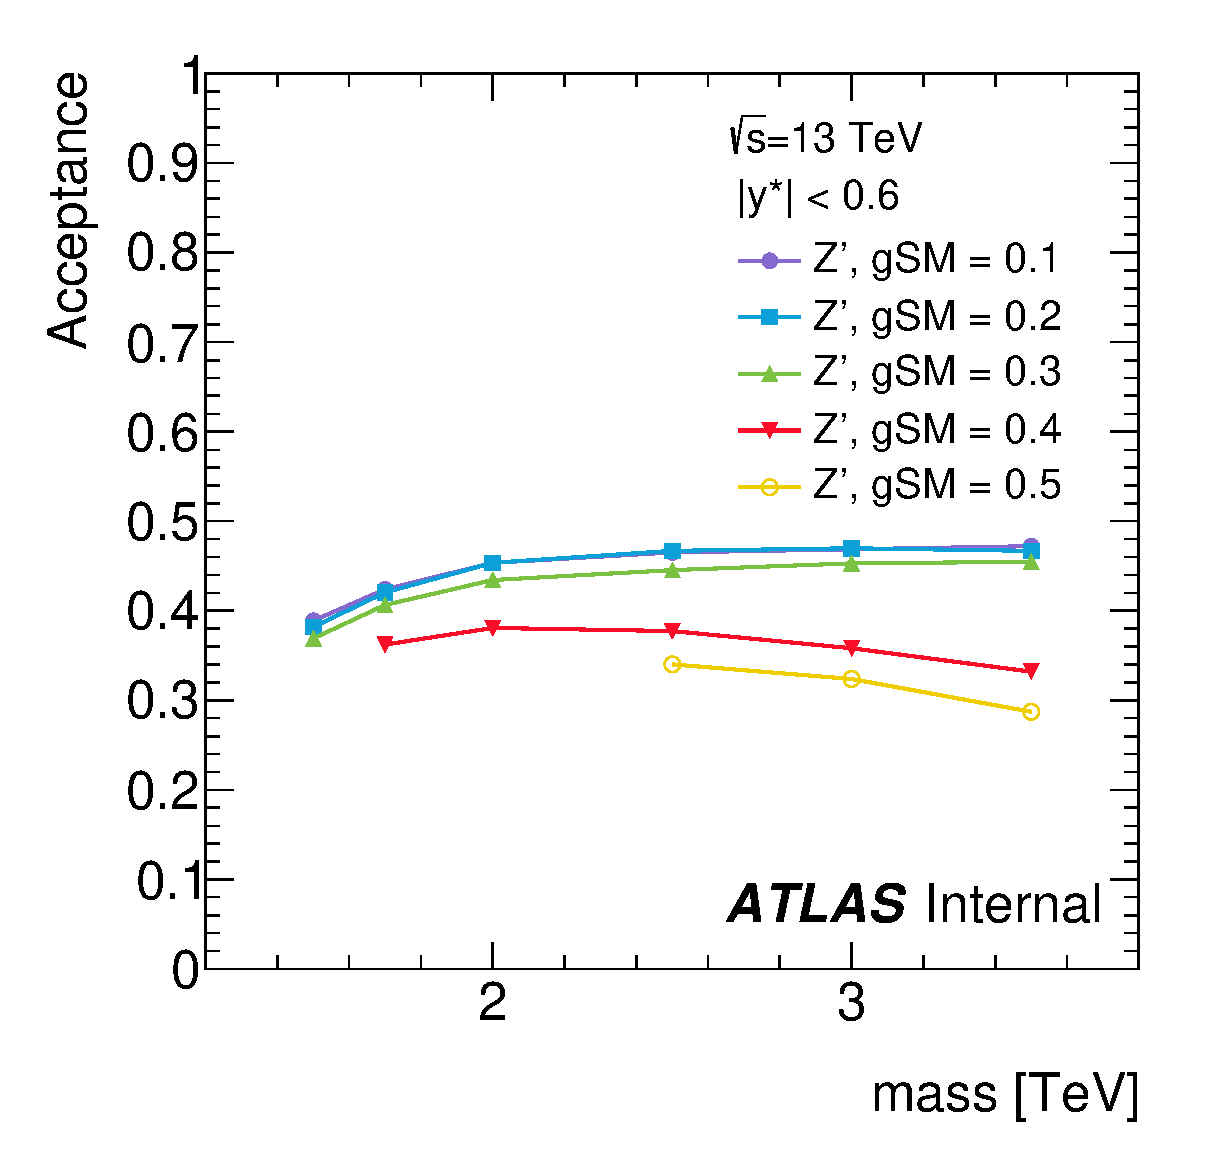
\includegraphics[width=0.45\textwidth]{figures/benchmark_signals/Acceptances_AllZPrime.eps}
%   \caption{Acceptance for the \Zprime\ models 
%   for 13~\TeV~center-of-mass energies using the full resonance
%   analysis selection (Section~\ref{sec:event_selection}).
%   \label{fig:zprime_acc}}
% \end{figure}
% 
% \clearpage
%\subsubsection{\Wstar\ Model}
%\label{sec:Wstar}
%
% A search has been performed for a \Wstar, a chiral excitations of the W boson, described in \cite{Chizhov:2010jg}, with further theoretical motivation in \cite{Chizhov:2009fc}. The presence of such an excited boson could be the evidence of W-boson compositeness. These excitations would couple to $qg$ final states and would lead to resonances in the dijet invariant mass spectrum. Their angular distributions would differ strongly from those of all other models considered here, with a $cos^{2}\theta$ dependence that produces an excess focused more towards the forward region. 
%
% A simplified model \cite{Chizhov:2010ry}, with the Lagrangian available in the CalcHEP 3.6 generator, has been utilised in the current studies. Using the NNPDF23$\_$nlo PDF, \Wstar event samples have been generated for masses ranging from 1.8 TeV to 4.0 TeV in steps of 200 GeV, which are then passed to Pythia8 for hadronisation. 
%
%The Langrangian of this Model is shown in equation (\ref{L}) where $\sin \theta_{X}$ is the mixing angle.
%
%\begin{eqnarray}\label{L}
%{\cal L}_{ref}&=&\frac{g}{\sqrt{2}M_{Z^*_d}}\left(
%\bar{d}\sigma^{\mu\nu}d+\bar{e}\sigma^{\mu\nu}e
%\right)\partial_\mu Z^*_{d\nu}+
%\frac{\sqrt{2}g}{\sqrt{3}M_{Z^*_u}}\left(\bar{u}\sigma^{\mu\nu}\!u\;
%\partial_\mu {\mathrm Re}Z^*_{u\nu}+
%i\,\bar{u}\sigma^{\mu\nu}\gamma^5\!u\;
%\partial_\mu {\mathrm Im}Z^*_{u\nu}\right) \nonumber\\
%&&\hspace{-0.8cm}+\frac{g}{M_{W^*}}\left(\sin\theta_X\,\overline{u_L}\sigma^{\mu\nu}d_R+
%\frac{2}{\sqrt{3}}\cos\theta_X\,\overline{u_R}\sigma^{\mu\nu}d_L+
%\sin\theta_X\,\overline{\nu_L}\sigma^{\mu\nu}e_R
%\right)\partial_\mu W^{*+}_{X\nu} + {\mathrm h.c.},
%\end{eqnarray}
%
%\Wstar\ samples can be generated using two different mixing angles.
%\begin{itemize}
%\label{sec:WstarSamples}
%\item Using mixing angle ($\sin \theta_X$) = 1 which favours leptonic decay. This leads to lower senstivity to dijet channel but can be used to compare the results with di-lepton final states.
%\item Using mixing angle ($\sin \theta_X$) = 0 which is lepto-phobic and favours jets as a final state. The advantage of using this condition is to have increase in sensitivity of the search  in dijet final states. 
%\end{itemize}
%
%\Wstar\ states were generated with lepto-phobic mixing angle ($\sin \theta_X$)=0 in this study because of the higher sensitivity of dijet final states in these models.
%
%
%Figures~\ref{fig:Wstar_xsec} and~\ref{fig:Wstar_acc} show the cross sections and
%acceptances as a function of the signal mass point.  
%The acceptance shown for the \Wstar\ model for 13 TeV~center-of-mass energies 
%uses the full resonance analysis selection for \Wstar\ signal (Section~\ref{sec:event_selection} where |y*|<1.2).
%
%\begin{figure}[!htb]
%  \centering
%  \subfigure[Cross section]{\label{fig:Wstar_xsec}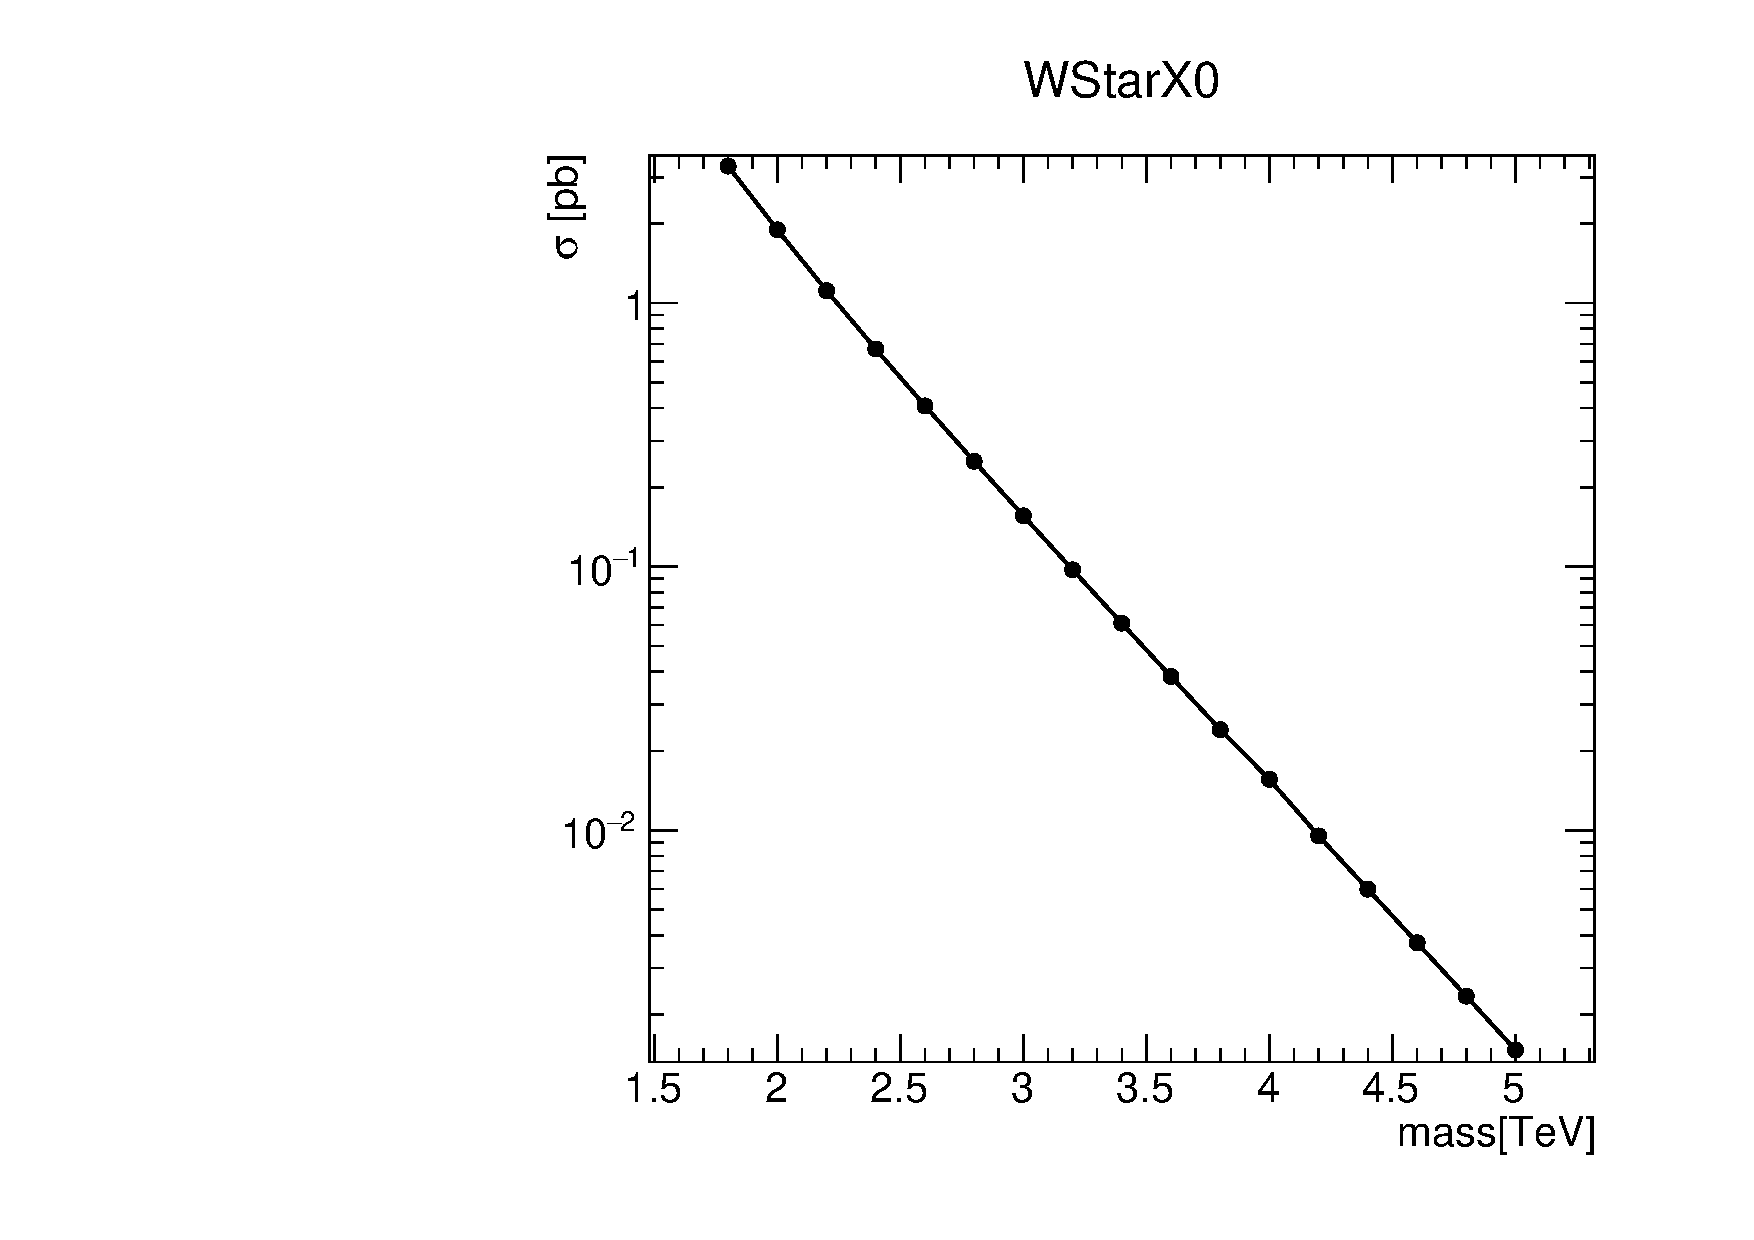
\includegraphics[width=0.48\textwidth]{figures/Wstar/CrossAcceptance/WstarX0_XS.pdf}}
%  \subfigure[Acceptance]{\label{fig:Wstar_acc}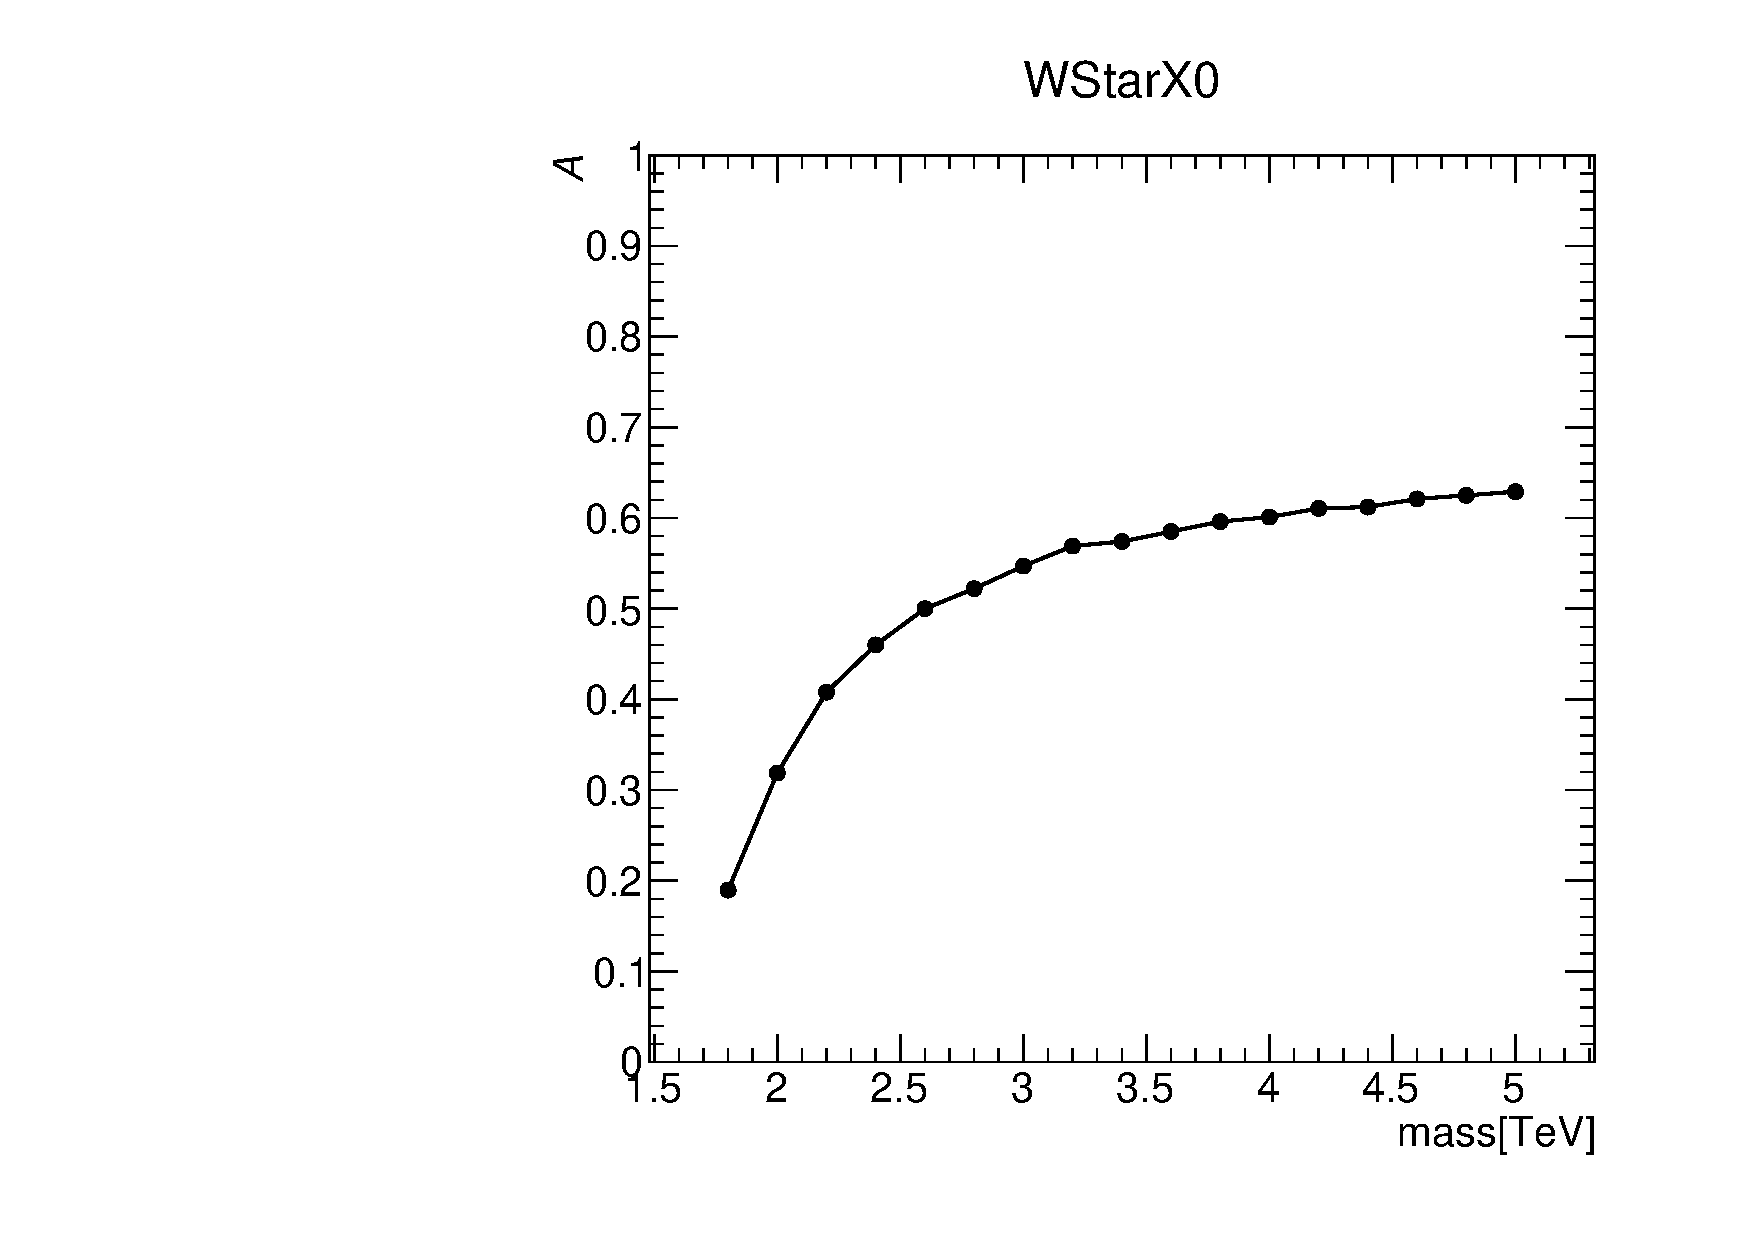
\includegraphics[width=0.48\textwidth]{figures/Wstar/CrossAcceptance/WstarX0_Acc.pdf}}
%	\caption{(a) Cross section and (b) acceptance for the 
%		\Wstar\ model for 13 TeV center-of-mass energies using the full resonance analysis selection (Section~\ref{sec:event_selection} except |y*|<1.2).
%		%   The interpolation between points is a straight line therefore the 
%		%   acceptance between m=1~\TeV~and m=2~\TeV~is not an accurate representation of
%		%   what the acceptance of a m=1.5~\TeV~sample would be.  The interpolation
%		%   is not used but drawn to help guide the eye.
%        }
%\end{figure}
%
%
%%%%%%%%%%%%%%%%%%%%%%%%%%%%%%%%%%%%%%%%%%%%%%%%%%%%%%%%%%%%%%%%%%%%%%%%%%%%%%%%%
% \clearpage
%
The quadratically divergent corrections to the Higgs self-energy is a
well known problem of the Standard Model.
Supersymmetry offers a solution to this problem by fine-tuning the
cancellation. 
Alternatively, in low-scale string theory quadratic divergences are 
cutoff by the string mass scale, thus avoiding the fine-tuning problem.
In addition, superstring theory can act as a unifying framework between
TeV-scale Standard Model physics and Planck-scale quantum gravity.  

Superstring theory provides a braneworld description of the Standard
Model, which is localized on membranes extending in $p+3$ spatial
dimension, the so-called D-branes of dimension $p$: D$p$-branes.
D-branes can thus be used to connect string theory to
phenomenology~\cite{Antoniadis:2000ena,Cremades:2002qm,Antoniadis:2002qm}.
Gauge bosons are due to strings attached to stacks of D-branes, and
chiral matter is due to strings stretching between intersecting D-branes.
The gauge interactions emerge as excitations of open strings with endpoints
attached on the D-branes, whereas gravitational interaction are described
by closed strings that can propagate in all nine spatial dimensions of
superstring theory.

We consider type-II string theory compactified on a six-dimensional
torus, which includes a D$p$-brane wrapped around $p-3$ dimensions of the
torus, with the remaining dimensions along our familiar (uncompactified)
three spatial dimensions.

The string mass-scale \Ms can be chosen hierarchically smaller than the
four-dimensional Planck scale at the expense of introducing $9-p$ large
transverse dimensions felt only by gravity, while keeping the string
coupling small~\cite{Cullen:2000ef}.
We are interested in the fundamental string scale in the TeV range.
The weakness of the effective four-dimensional gravity compared to gauge
interactions is then attributed to the large transverse space radii
compared to the string length; the so called AADD
model~\cite{ArkaniHamed:1998rs,Antoniadis:1998ig}. 

The string coupling must be small for the validity of the above D-brane
framework and of perturbation theory in the computation of scattering
amplitudes. 
If AADD is valid, string resonances will likely appear before gravity
signatures.
In this case, black hole production and other strong gravity effects
occur at energies above the string scale.
Thus, at least the lowest few Regge recurrences, are available for
examination, free from interference with some complex quantum
gravitational phenomena. 
The dominance of string resonances over Kaluza-Klein effects and winding
states is a generic feature of weakly coupled string
theory~\cite{Cullen:2000ef}. 
We do not considering the Kaluza-Klein states of the graviton in the
extra dimensions or the winding states.

In this framework, a whole tower of infinite string excitations will
open up at this low-mass threshold, and new particles of spin $J$ will
follow the well-known Regge trajectories of vibrating
strings.  
The string mass scale determines the centre of mass energy threshold 
for the production of Regge resonances in parton collisions, thus
corresponds to the onset of string effects at the LHC.

We consider dominant subprocesses in dijet production that are
independent of the details of compactification and are essentially
parameter free. 
Amplitudes, which include $2\to 2$ scattering processes involving four
gluons, or two gluons and two quarks, are independent of the details of
the compactification such as the configuration of branes, the geometry
of the extra dimensions, and whether SUSY is broken or
not~\cite{Lust:2008qc}. 
This model independence makes it possible to compute the string
corrections to QCD dijet processes.

The string resonances occur at masses $m_n = \sqrt{n} \Ms$, for $n = 1,
2, 3, \ldots$.
We only consider the first $(n=1)$ resonant pole.
The resonance will consist of a combination of the Regge excitations of
the quark, the gluon, and the colour singlet living on the QCD stack of
branes. 
The string-resonance widths have been calculated in
Ref~\cite{Anchordoqui:2008hi}. 

First phenomenological studies were done in
Ref~\cite{Anchordoqui:2007da,Anchordoqui:2009mm,Kitazawa:2010gh,Anchordoqui:2014wha}. 
Searches for string resonances have been performed in previous dijet
mass spectra.
ATLAS~\cite{ATLAS:2012pu} searched in 4.8~fb$^{-1}$ of data at $\sqrt{s}
= 7$~TeV.
A lower limit of $\Ms < 3.61$~TeV at a 95\% CL was set.
The MC signal samples were provided by a non-ATLAS member Noriaki
Kitazawa who used CalcHEP.
CMS~\cite{Chatrchyan:2011ns,CMS:2012yf} performed two searches in dijets
at $\sqrt{s} = 7$~TeV.
Lower limits of $\Ms < 4.00$~TeV and $\Ms < 4.31$~TeV were set at the
95\% CL using datasets of 1.0~fb$^{-1}$ and 5.0~fb$^{-1}$, respectively. 
It is not totally clear how this limit was set but the excited
quark MC sample was probably used for the signal event generation. 
A non-CMS member Can Kilic did the string resonance cross section
calculation. 
CMS~\cite{Khachatryan:2015sja} performed the only search at $\sqrt{s} =
8$~TeV using 19.7~fb$^{-1}$ of data, to obtain a lower limit of $\Ms <
5.0$~TeV at the 95\% CL.
The paper does not explanation of how this limit was calculated.
CMS~\cite{Khachatryan:2015dcf,Sirunyan:2018xlo} performed two searches
in dijets at $\sqrt{s} = 13$~TeV. 
Lower limits of $\Ms < 7.0$~TeV and $\Ms < 7.7$~TeV were set at the
95\% CL using datasets of 2.4~fb$^{-1}$ and 36~fb$^{-1}$, respectively. 
Again, no explanation of the signal samples are given and only the $gq$
state is considered.
Both experiments have performed searches for string balls in different
decay modes at $\sqrt{s} = 7, 8$, and 13~TeV, but we argue that the
model~\cite{Gingrich:2008di} used does not constrain string resonances,
or visa versa. 
%%%%%%%%%%%%%%%%%%%%%%%%%%%%%%%%%%%%%%%%%%%%%%%%%%%%%%%%%%%%%%%%%%%%%%%%%%%%%%%%%

%%%%%%%%%%%%%%%%%%%%%%%%%%%%%%%%%%%%%%%%%%%%%%%%%%%%%%%%%%%%%%%%%%%%%%%%%%%%%%%%%
Five string-resonance samples with string scales \Ms from 7.0~TeV to
9.0~TeV, in steps of 0.5~TeV are generated.
The minimum mass $M_\mathrm{min}$ used in the generator and the
resulting cross section of the samples are shown in Table~\ref{tab1}. 

\begin{table}[htb]
\begin{center}
\begin{tabular}{ccc}\hline\\[-2ex]
\Ms & $M_\mathrm{min}$ & Cross section\\
{[TeV]} & {[TeV]} & {[fb]}\\ \\[-2ex]
\hline\\[-2ex]
7.0 & 6.06 & $7.09\times 10^{+0}$\\
7.5 & 6.60 & $1.86\times 10^{+0}$\\
8.0 & 7.14 & $4.56\times 10^{-1}$\\
8.5 & 7.60 & $1.00\times 10^{-1}$\\
9.0 & 8.05 & $1.99\times 10^{-2}$\\
\\[-2ex]\hline
\end{tabular}
\end{center}
\caption{Monte Carlo string-resonance samples with string scale \Ms,
minimum mass $M_\mathrm{min}$, and cross section.} 
\label{tab1}
\end{table}

The string resonances have long Breit-Wigner tails and the lower-mass
tail can be significantly enhanced by the PDFs at low-$x$ (low mass).
Since we are interested in a narrow-resonance structure in the dijet
mass distribution, we truncate the low-mass tail.
For the $7.0 \leq \Ms \leq 8.0$~TeV samples, we truncate at the minimum in
the differential cross section on the lower-mass side of the \Ms peak,
which results in including slightly more than 95\% of the area under the
curve. 
For the $8.5 \leq \Ms \leq 9.0$~TeV samples, we truncate at a lower-mass
value that covers 95\% of the area under the Breit-Wigner curve.

Five possible $2\to 2$ subprocesses that can give rise to string
resonances are simulated.
The cross section for each subprocess is a function of \Ms, and thus the
relative contribution of each subprocess to the total cross section varies
with \Ms, as shown in Table~\ref{tab2}.
The dominate subprocess at the \Ms values we consider is $gq\to gq$ which
contributes about 81-87\% of the total cross section.
Previous ATLAS and CMS searches only included the dominate subprocess.
The $qq\to qq$, $\bar{q}\bar{q}\to \bar{q}\bar{q}$, and $q\bar{q}\to
q\bar{q}$ subprocesses are model dependent, and not
considered here.

\begin{table}[htb]
\begin{center}
\begin{tabular}{crrrrr}\hline\\[-2ex]
Subprocess             & \multicolumn{5}{c}{\Ms\ {[TeV]}}\\
& \multicolumn{1}{c}{7.0} & \multicolumn{1}{c}{7.5} &
\multicolumn{1}{c}{8.0} & \multicolumn{1}{c}{8.5} &
\multicolumn{1}{c}{9.0}\\ \\[-2ex]
\hline\\[-2ex]
$gg\to gg$             & 11.36\% &  9.52\% &  8.17\% &  7.23\% &  5.07\%\\
$gg\to q\bar{q}$       &  0.29\% &  0.28\% &  0.22\% &  0.19\% &  0.17\%\\
$gq\to gq$             & 81.36\% & 83.12\% & 84.58\% & 85.54\% & 87.59\%\\
$g\bar{q}\to g\bar{q}$ &  0.68\% &  0.58\% &  0.52\% &  0.51\% &  0.49\%\\
$q\bar{q}\to gg$       &  6.31\% &  6.50\% &  6.51\% &  6.53\% &  6.67\%\\
\\[-2ex] \hline
\end{tabular}
\end{center}
\caption{String-resonance subprocesses and their relative contribution
to the total cross section for different string scales \Ms.
The statistics are based on samples of 66000 events.}
\label{tab2}
\end{table}

For the string-resonance samples, the MC event
generator \str~1.00~\cite{Vakilipourtakalou:2018pfo} is used.
It is interfaced to \pythia~8.240~\cite{Sjostrand:2014zea} for modelling
of the parton shower, hadronization, and underlying event, with
parameters from the A14 tune~\cite{ATL-PHYS-PUB-2014-021}.
The leading-order CTEQ6L1~\cite{Pumplin:2002vw} PDF set is used for the
parton shower and the hard-scattering process.
The EvtGen~1.6.0 program~\cite{Lange:2001uf} is used to decay bottom
and charm hadrons. 

The effect of multiple interactions in the same and neighbouring bunch
crossings (pile-up) is modelled by overlaying simulated inelastic $pp$
events generated with \pythia~8.186~\cite{Sjostrand:2014zea}
using NNPDF2.3LO set of PDFs~\cite{Ball:2012cx} and the A3
tune~\cite{ATL-PHYS-PUB-2016-017} over the original hard-scattering event. 
%%%%%%%%%%%%%%%%%%%%%%%%%%%%%%%%%%%%%%%%%%%%%%%%%%%%%%%%%%%%%%%%%%%%%%%%%%%%%%%%%
%
%\clearpage
%\subsubsection{Signal shapes in the various models}
%
%The shape of the signal peak for each mass point and each signal model, after the resonance selection cuts, are shown in Figure~\ref{fig:showallshapes}. Each template is normalised to 1, and therefore differences in peak amplitude are indicative of a broadening or narrowing of the signal rather than of a change in cross section.
%\begin{figure}[!htb]
%\centering
%\subfigure[q* model]{\label{fig:resonance_templates_2500}
%               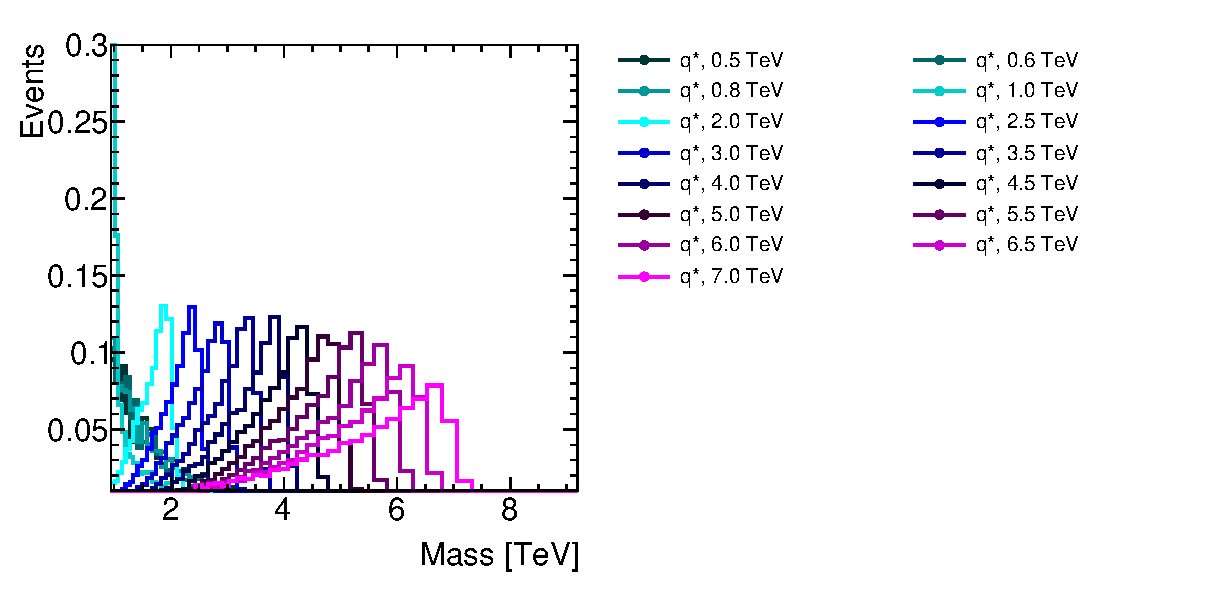
\includegraphics[height=0.25\textwidth]{figures/benchmark_signals/overlaidQStar_mjj_linear.eps}}
%\subfigure[\BlackMax\ model]{\label{fig:resonance_templates_4500}
%               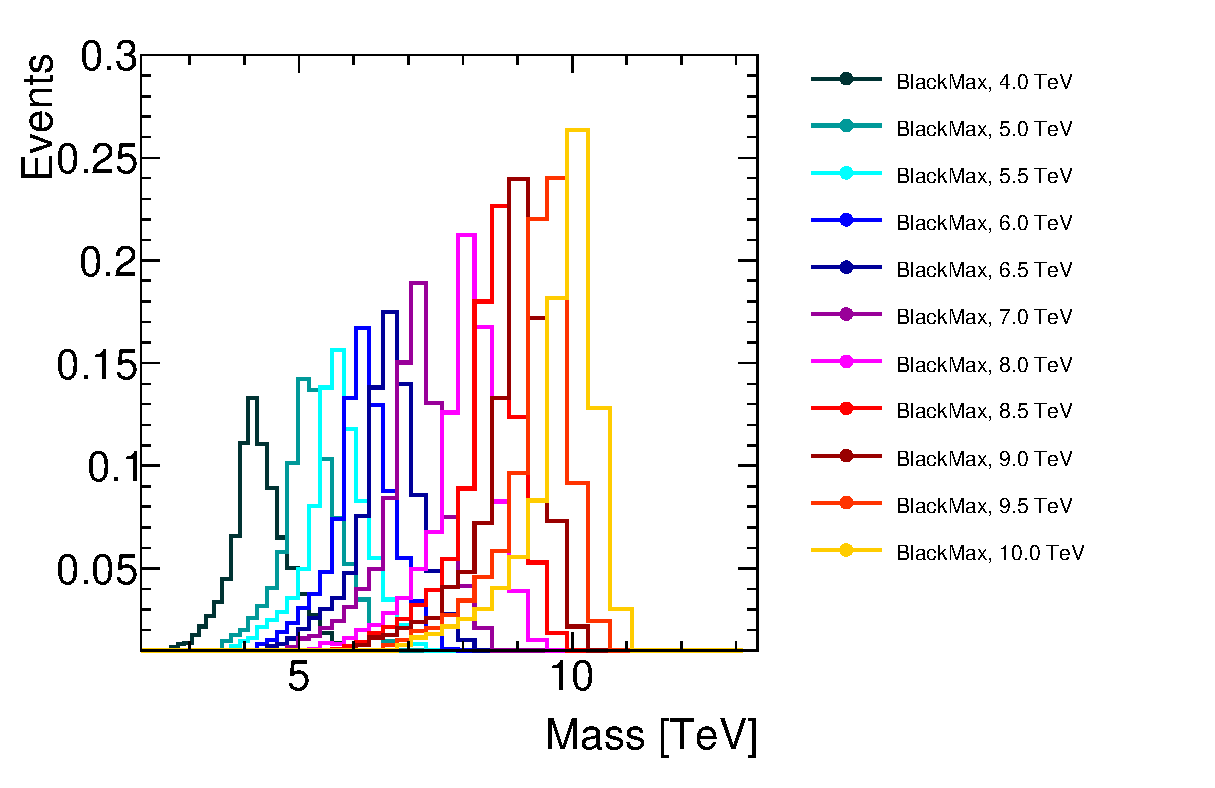
\includegraphics[height=0.25\textwidth]{figures/benchmark_signals/overlaidBlackMax_mjj_linear.eps}}
%\subfigure[\Wprime\ model]{\label{fig:resonance_tr_templates_2500}
%               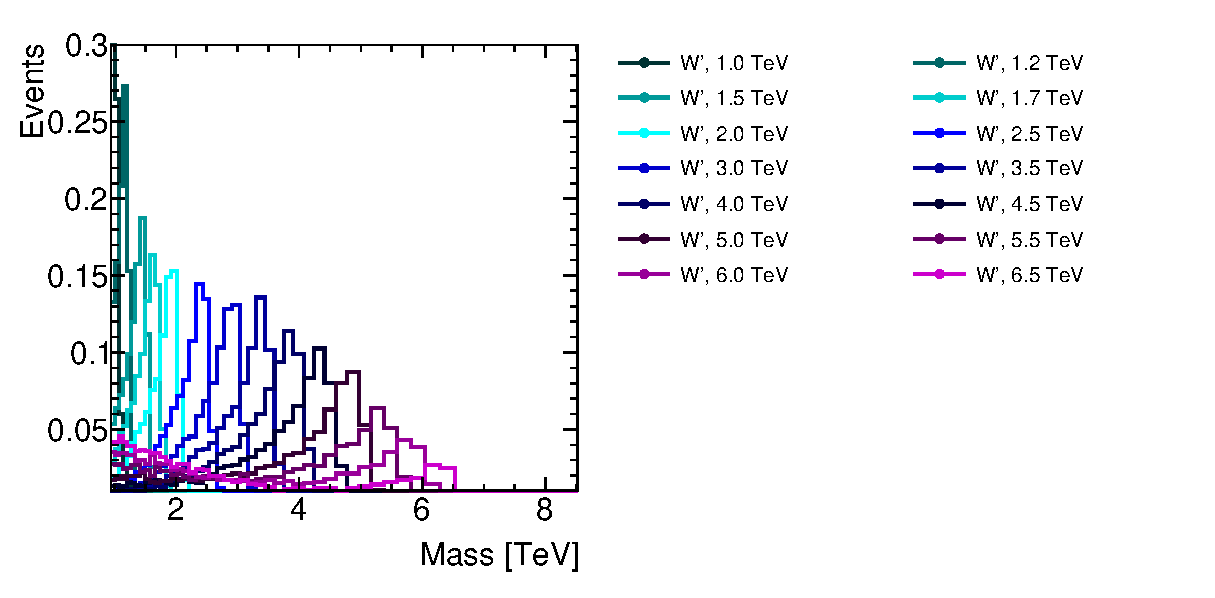
\includegraphics[height=0.25\textwidth]{figures/benchmark_signals/overlaidWPrime_mjj_linear.eps}}
%\subfigure[\Wstar\ model]{\label{fig:showallshapes}
%               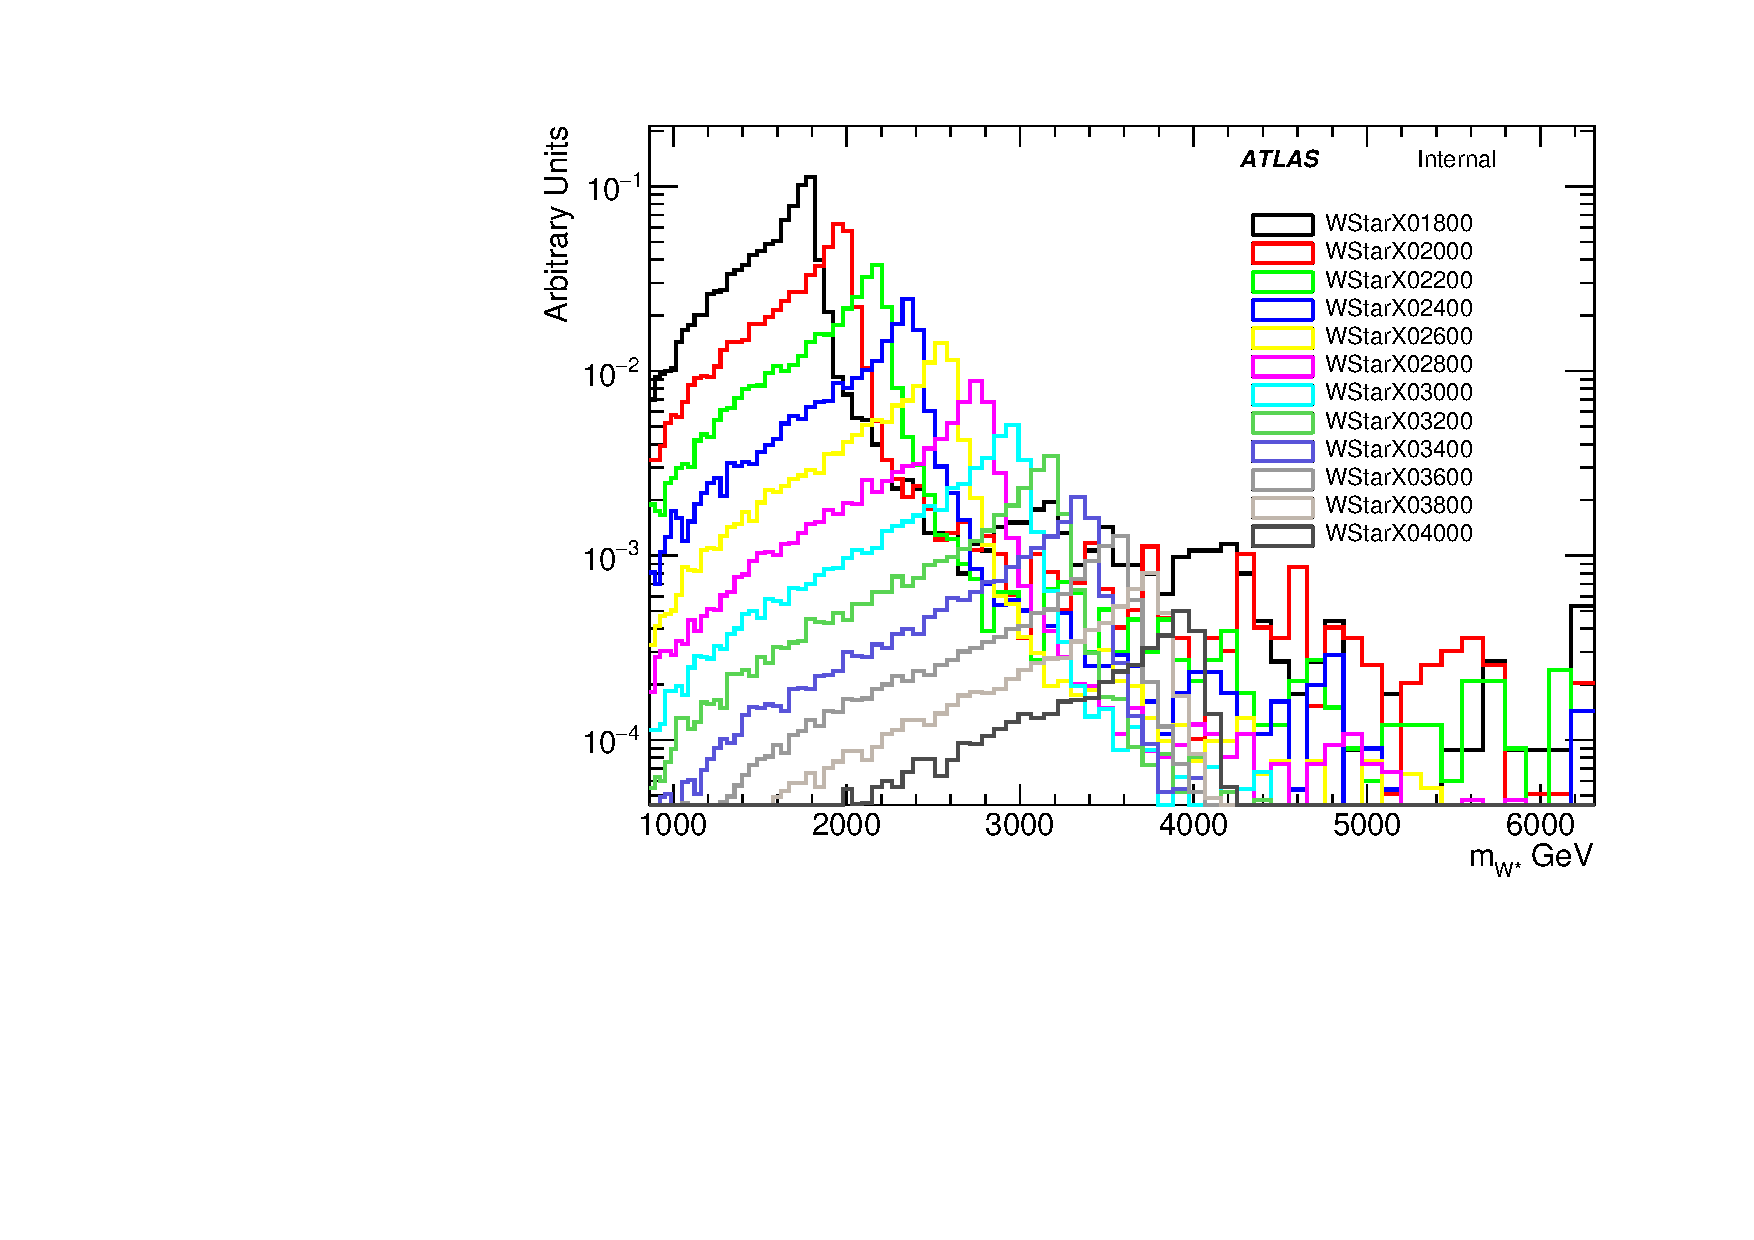
\includegraphics[height=0.25\textwidth]{figures/Wstar/CrossAcceptance/MassesDist.pdf}}
%%\subfigure[4.5 TeV, truncated]{\label{fig:resonance_tr_templates_4500}
% %              \includegraphics[width=0.45\textwidth]{old_figures_2015/search_results/Resonance/Gaus_Comp/M4500_tr_comp.pdf}}
%\caption{Normalized \mjj\ templates at every mass point considered in the limit setting phasse for each of the resonant benchmark models. }
%
%\end{figure}
%
%The benchmark signals used vary in their underlying physics motivation, but also in the resulting shape of the signal \mjj\ distribution. 
%This is demonstrated most clearly in Figure~\ref{fig:resonance_templates_shapes}, which shows overlaid reconstructed \mjj\ distributions for a selection of benchmark signals at the same mass point.
%The low-mass tail of \Wprime\ starts to become pronounced at higher masses, and the \qstar\ signal is also broadened. 
%In contrast to the previous two, \BlackMax\ signals peak at masses slightly higher than the generated mass. 
%The detailed differences between the signal shapes become apparent in Figures~\ref{fig:resonance_tr_templates_4000} and \subref{fig:resonance_tr_templates_6500}, 
%which show the signal templates truncated at $\pm 20 \%$ of the generated mass. 
%This is the truncation recommended for recasting of the generic Gaussian observed limits set by this analysis into signals with peaked but non-Gaussian \mjj\ distributions. 
%The truncated distributions show that the \qstar\ signal distributions are shifted the most to lower \mjj\ of all signals, for both lower and higher masses. 
%% 
%% 
%\begin{figure}[!htb]
%\centering
%\subfigure[4.0 TeV]{\label{fig:resonance_templates_4000}
%               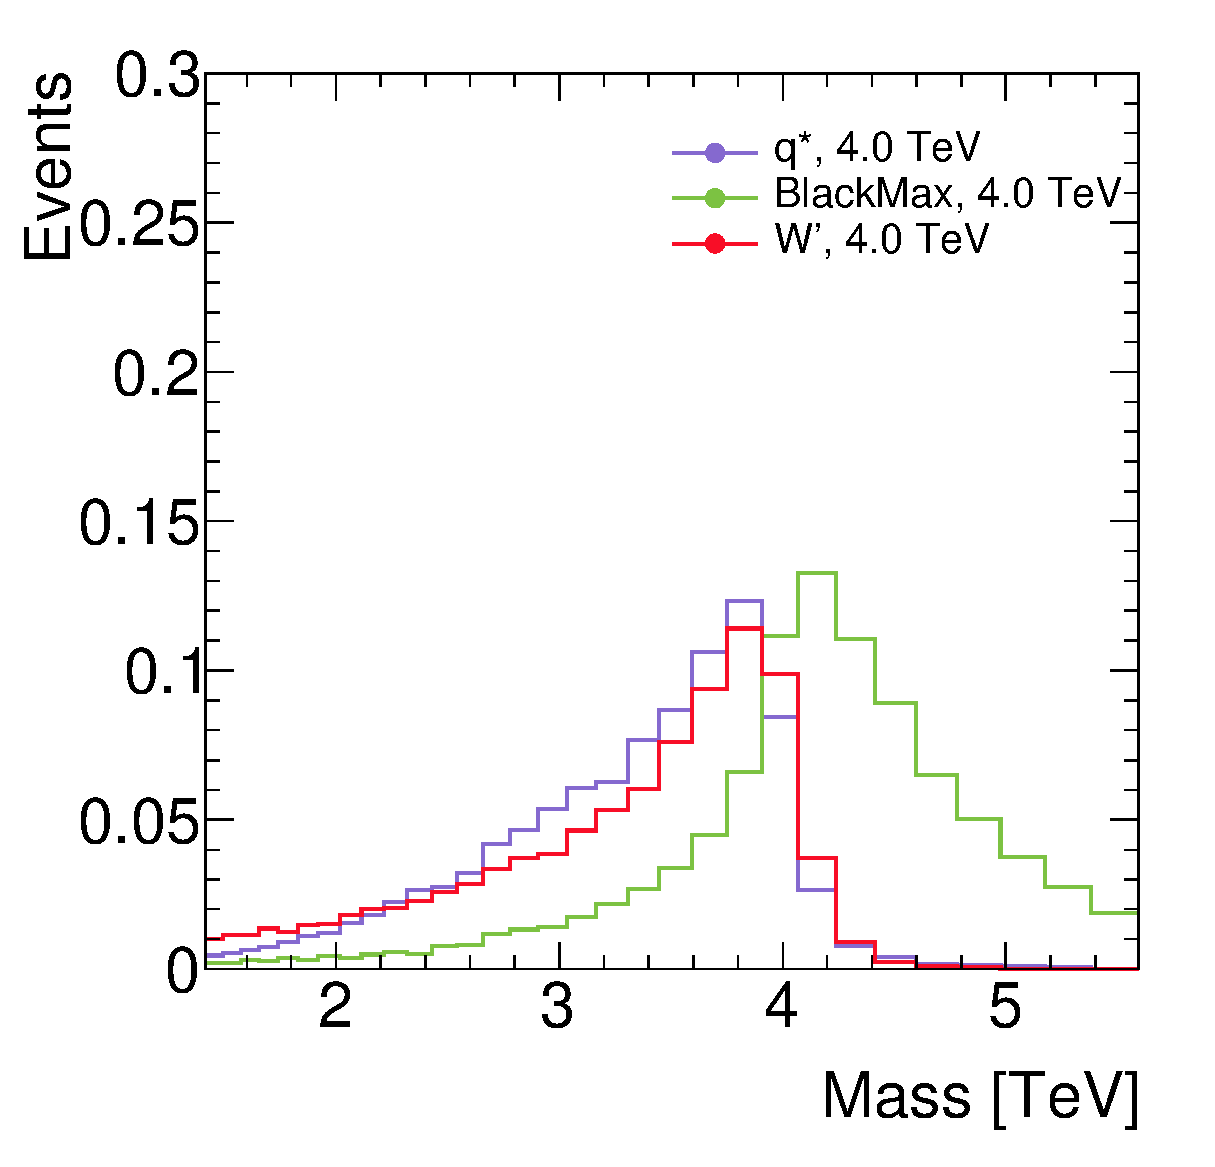
\includegraphics[width=0.45\textwidth]{figures/benchmark_signals/overlaidSignals_m4000_linear.eps}}
%\subfigure[6.5 TeV]{\label{fig:resonance_templates_6500}
%               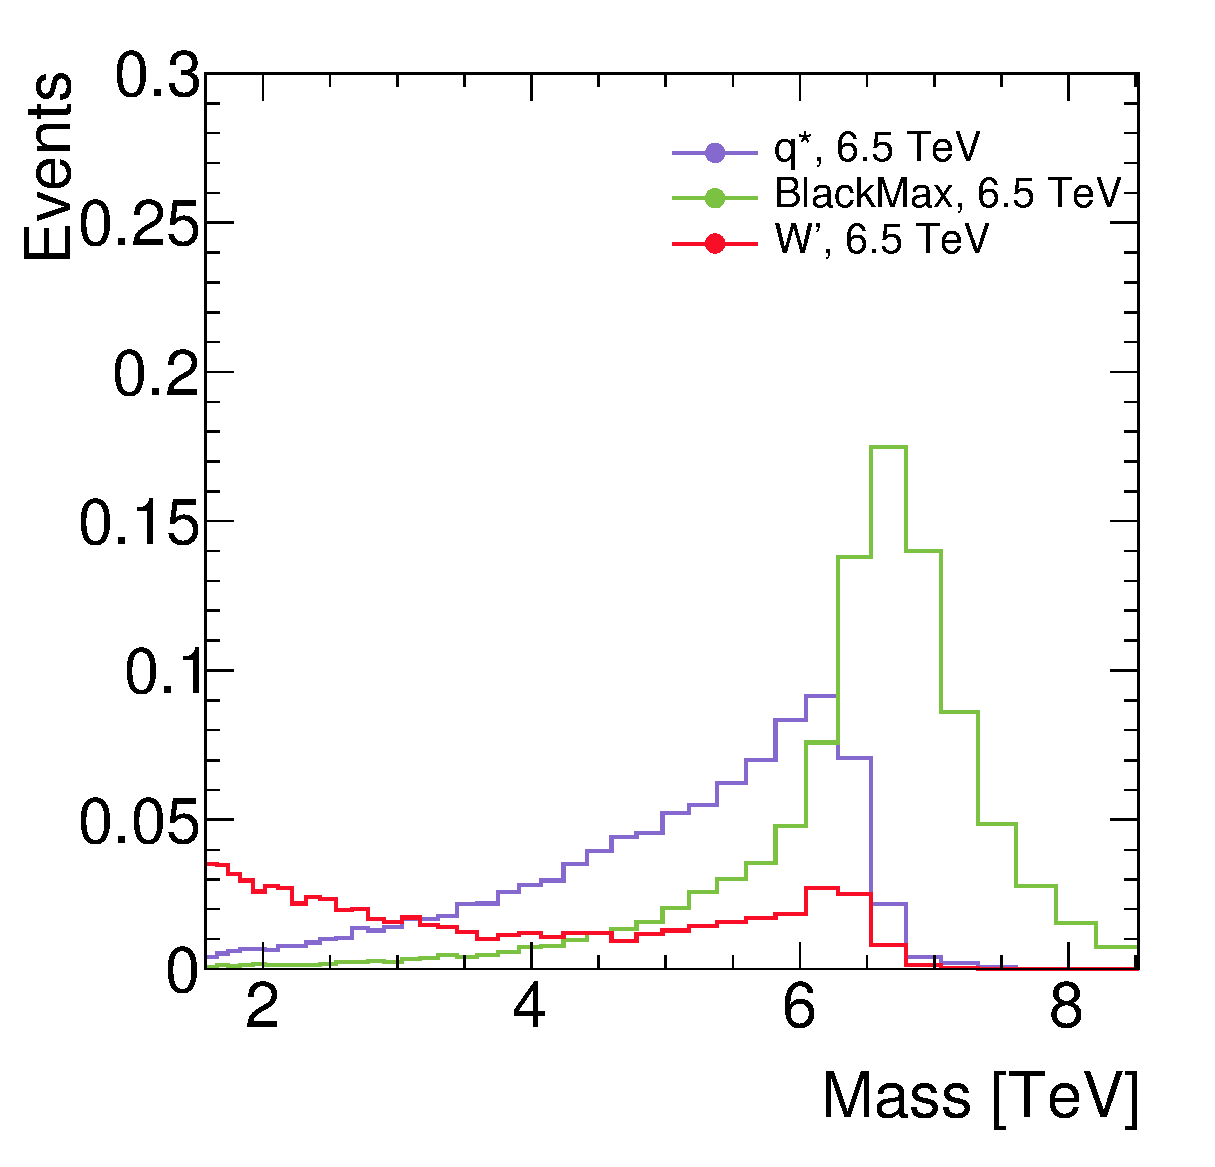
\includegraphics[width=0.45\textwidth]{figures/benchmark_signals/overlaidSignals_m6500_linear.eps}}
%\subfigure[4.0 TeV, truncated]{\label{fig:resonance_tr_templates_4000}
%               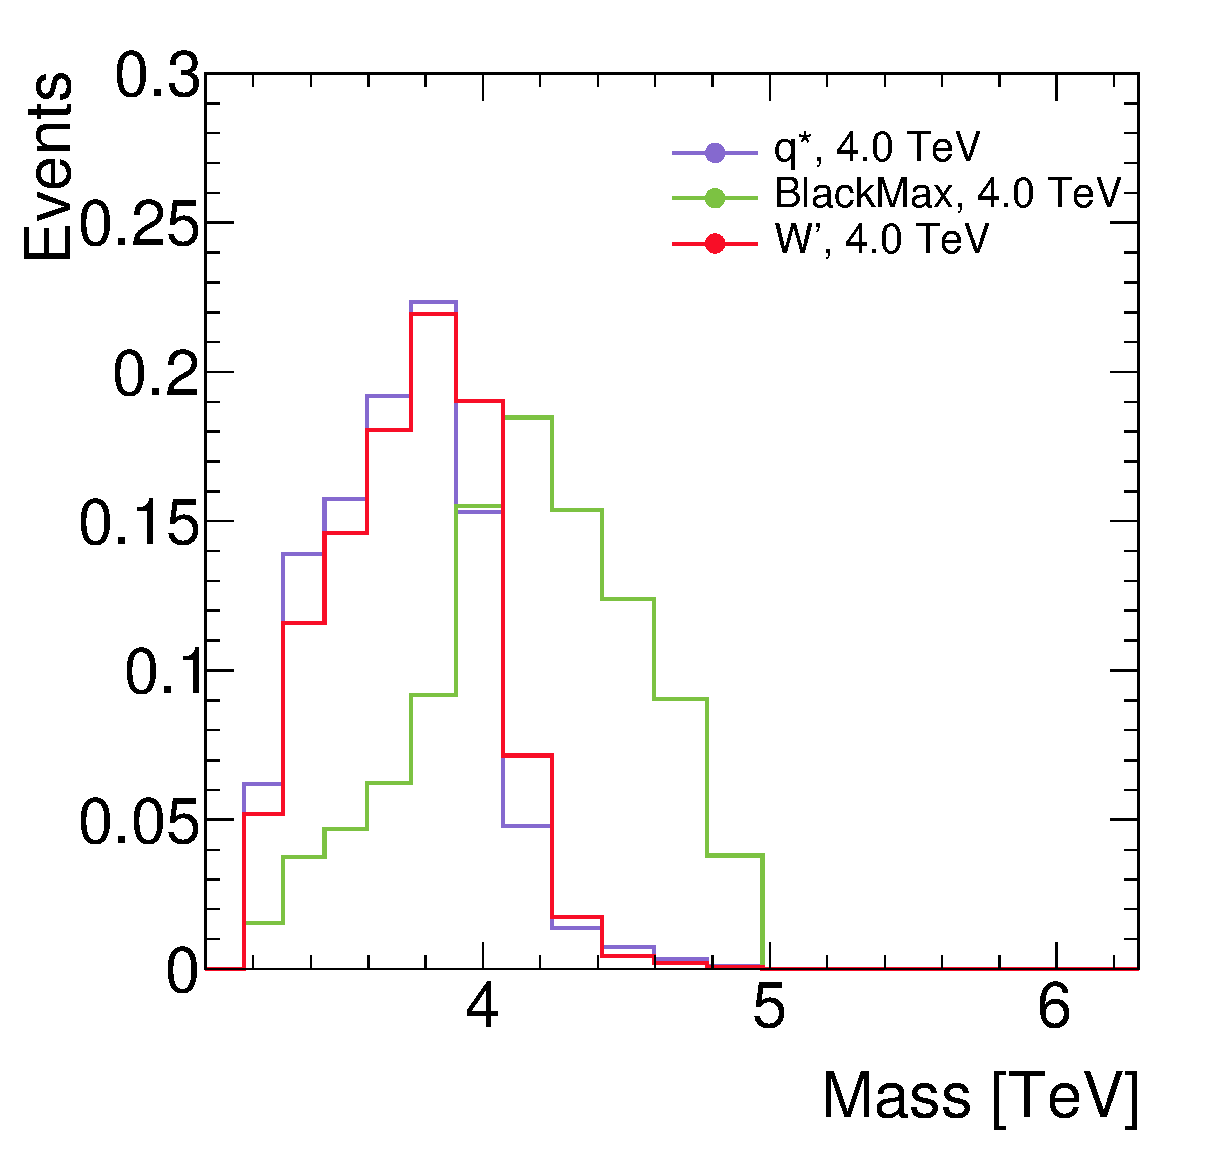
\includegraphics[width=0.45\textwidth]{figures/benchmark_signals/overlaidSignals_m4000_trunc.eps}}
%\subfigure[6.5 TeV, truncated]{\label{fig:resonance_tr_templates_6500}
%               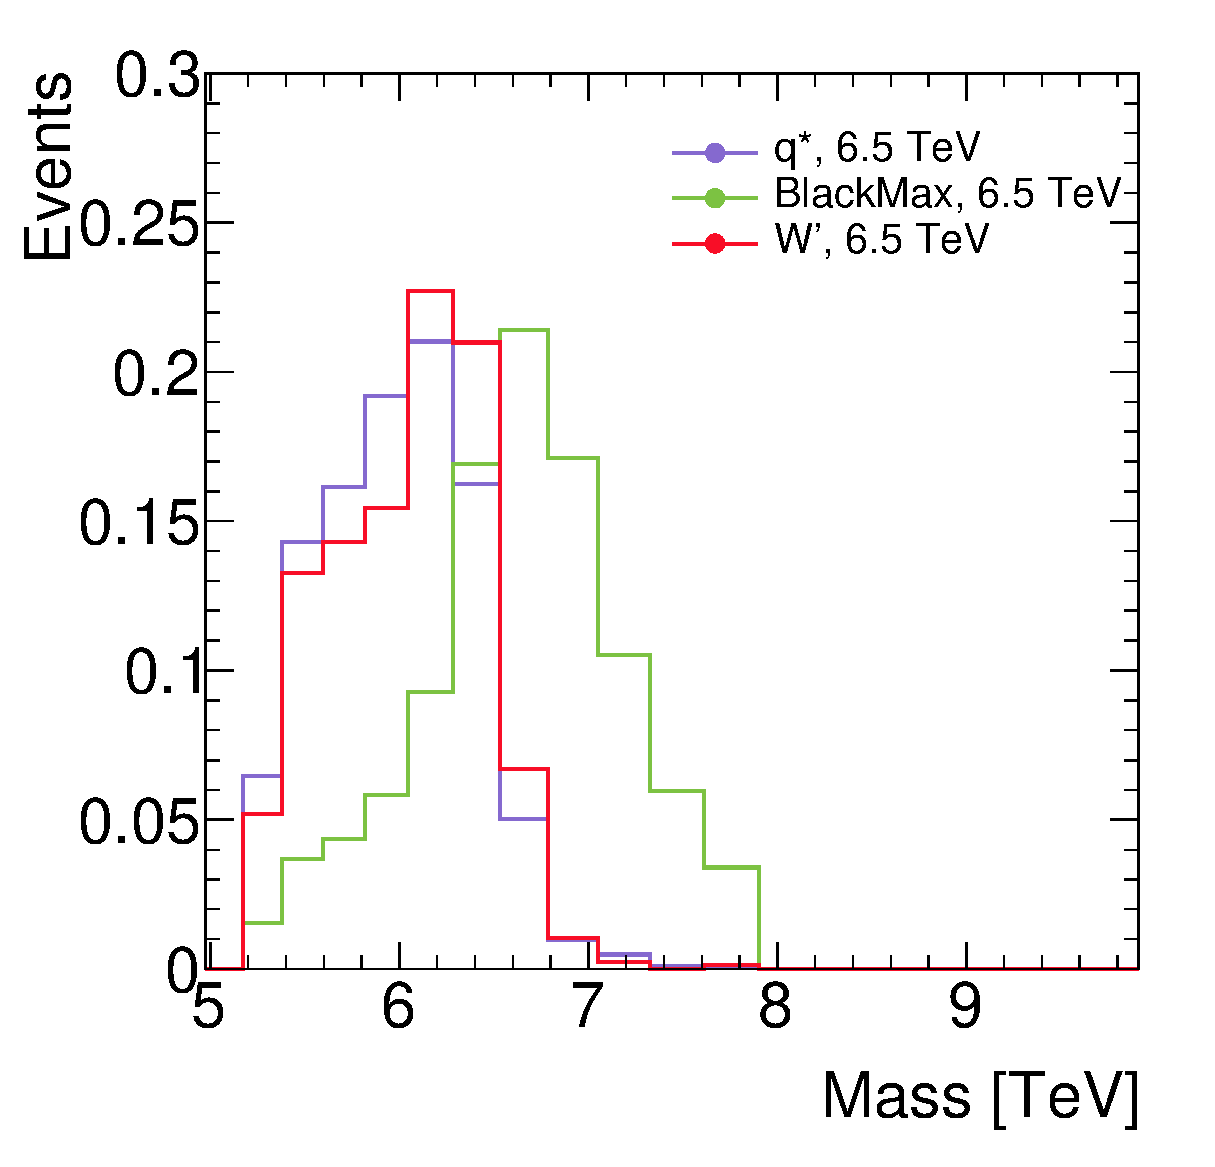
\includegraphics[width=0.45\textwidth]{figures/benchmark_signals/overlaidSignals_m6500_trunc.eps}}
%
%\caption{Normalized \mjj\ templates at 4.0 TeV \subref{fig:resonance_templates_4000},\subref{fig:resonance_tr_templates_4000} and 6.5 TeV \subref{fig:resonance_templates_6500},\subref{fig:resonance_tr_templates_6500}, before (above) and after (below) the truncation procedure, for various resonant benchmark models. The signals are re-normalised after truncation for ease of comparison of the shapes.}
%\label{fig:resonance_templates_shapes}
%\end{figure}
%

\clearpage
%%%%%%%%%%%%%%%%%%%%%%%%%%%%%%%%%%%%%%%%%%%%%%%%%%%%%%%%%%%%%%%%%%%%
\subsubsection{Signal Morphing}
\label{sec:SwiftMorphing}
%%%%%%%%%%%%%%%%%%%%%%%%%%%%%%%%%%%%%%%%%%%%%%%%%%%%%%%%%%%%%%%%%%%%


Smooth signal mass distributions are obtained  from morphing the signal shapes from MC. The MC signals are fit to a Gaussian + reverse Landau function, a parameterization that has one normalization and five shape parameters. The parameters are interpolated as a function of mass using cubic splines. This allows the use of signal shapes at any mass. Figure~\ref{fig:morphing} shows some examples of fits to MC signal shapes as well as several interpolated signal shapes.  

\begin{figure}[!htb]
	\centering
	\subfigure[q* signals]{ 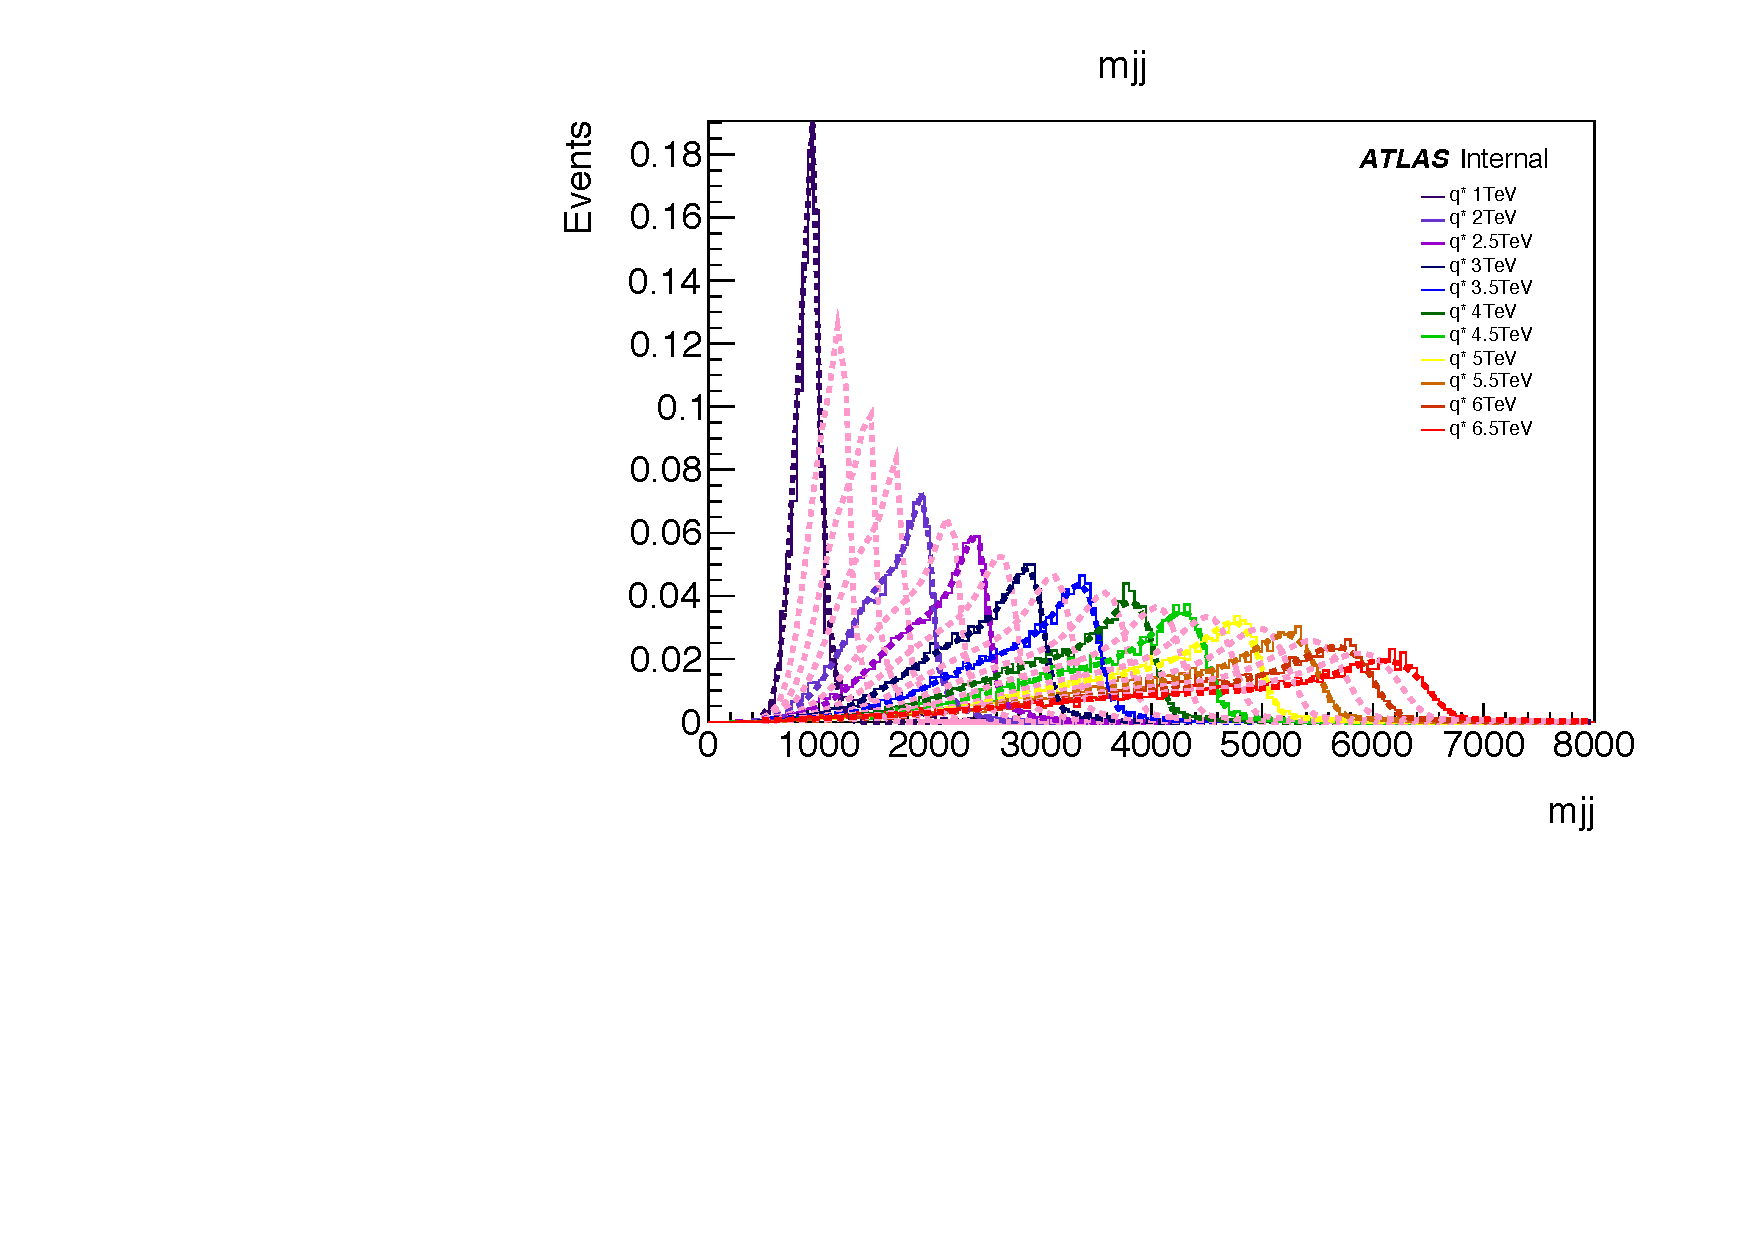
\includegraphics[width=0.48\textwidth]{figures/SWiFt/interpolate_qStar.pdf} }
	\subfigure[Reclustered W' signals]{ 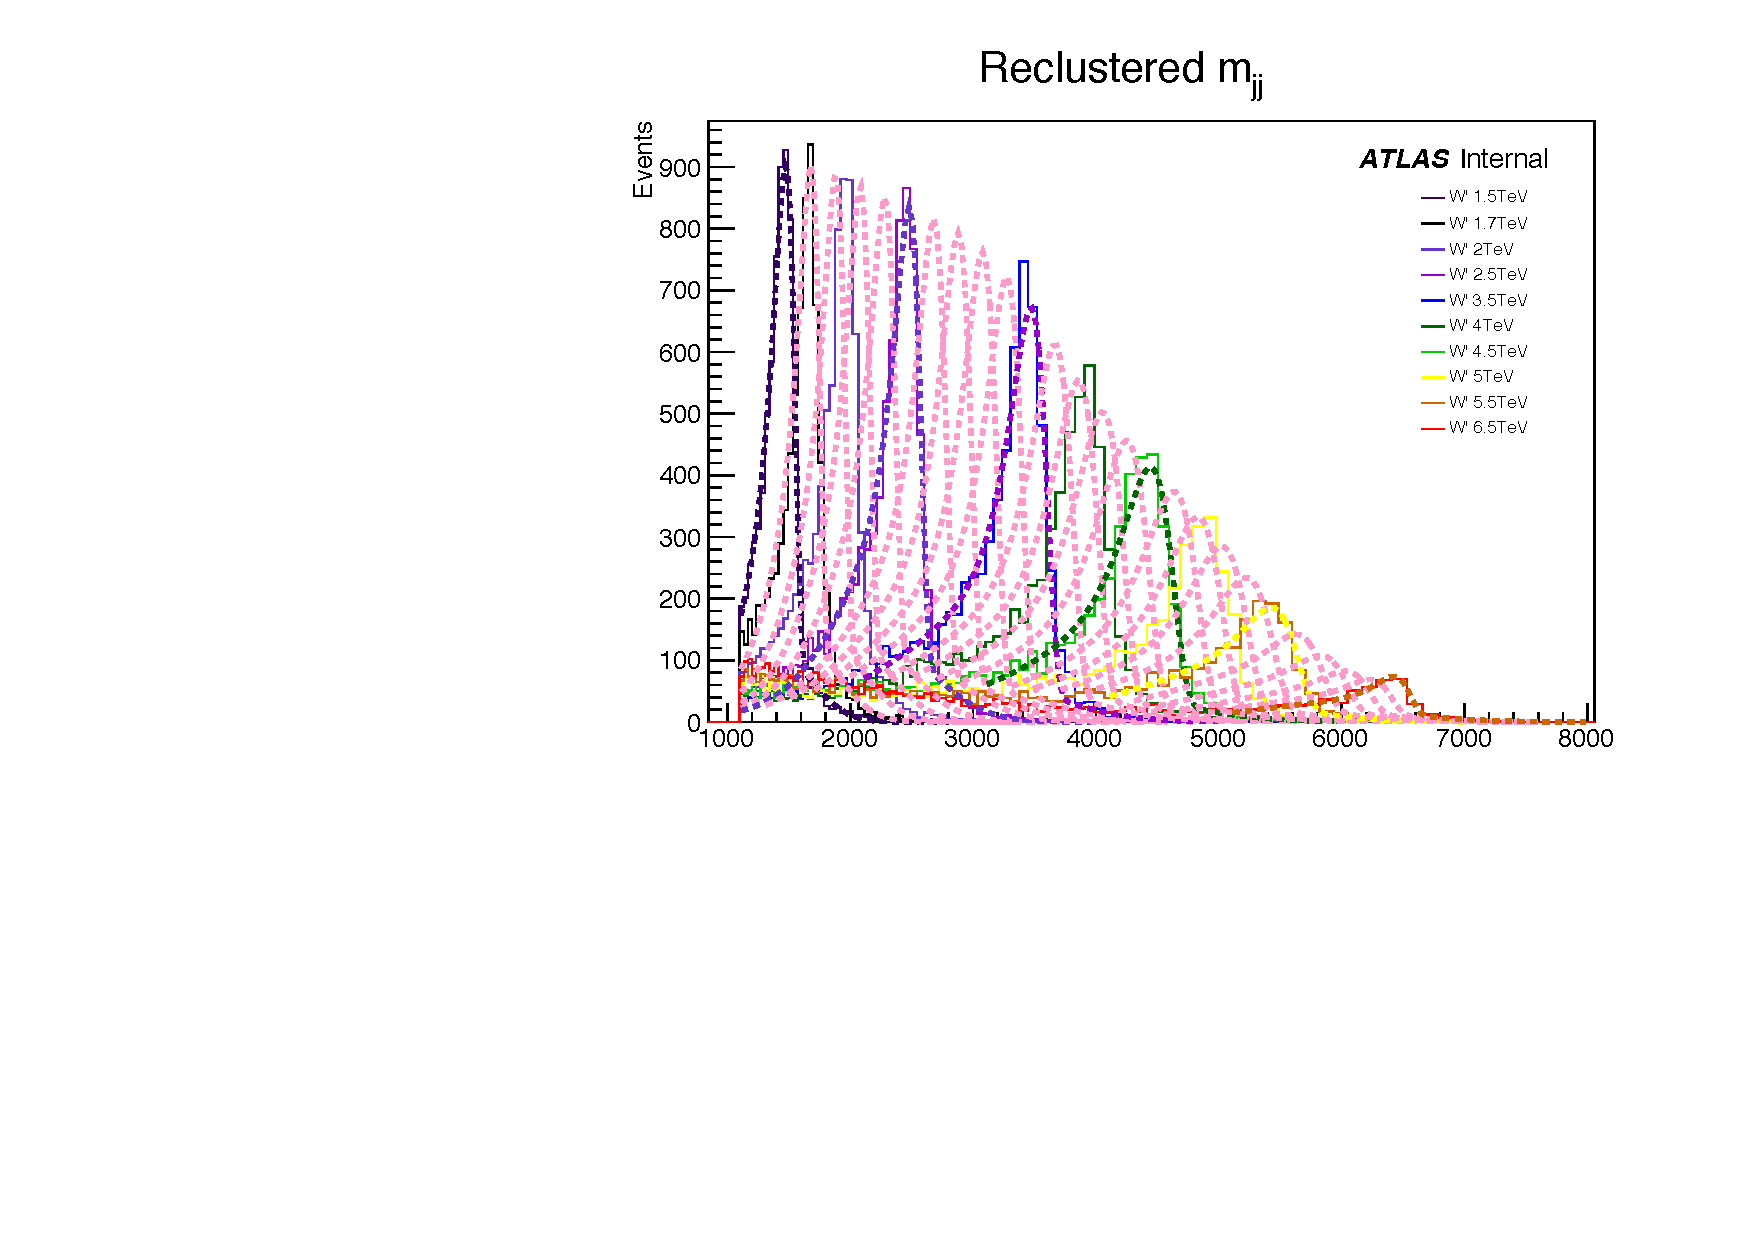
\includegraphics[width=0.48\textwidth]{figures/SWiFt/interpolate_WPrimeRe.pdf} }
	\subfigure[Z' 0.2 SM coupling signals]{ 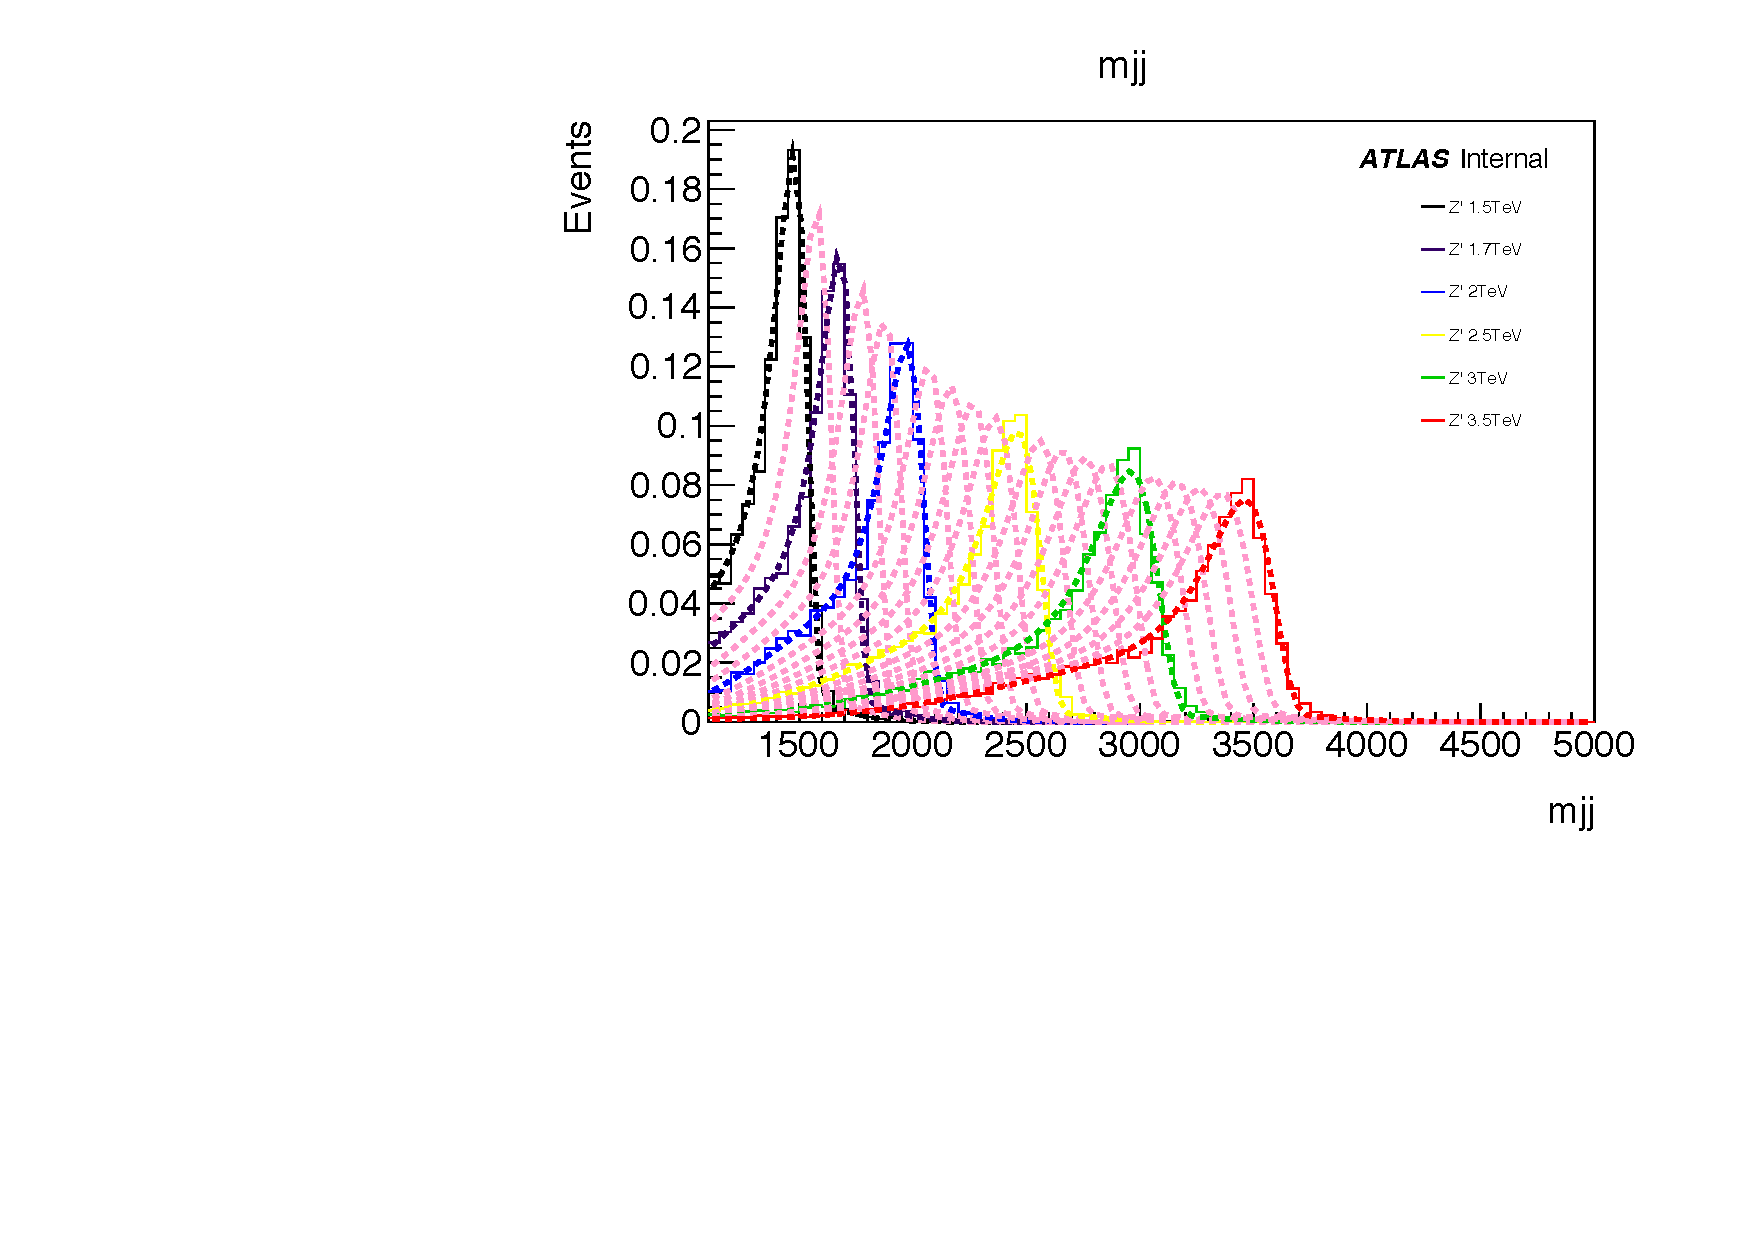
\includegraphics[width=0.48\textwidth]{figures/SWiFt/ZPrime_gSM0p20.pdf} }
	\subfigure[Z' 0.5 SM coupling signals]{ 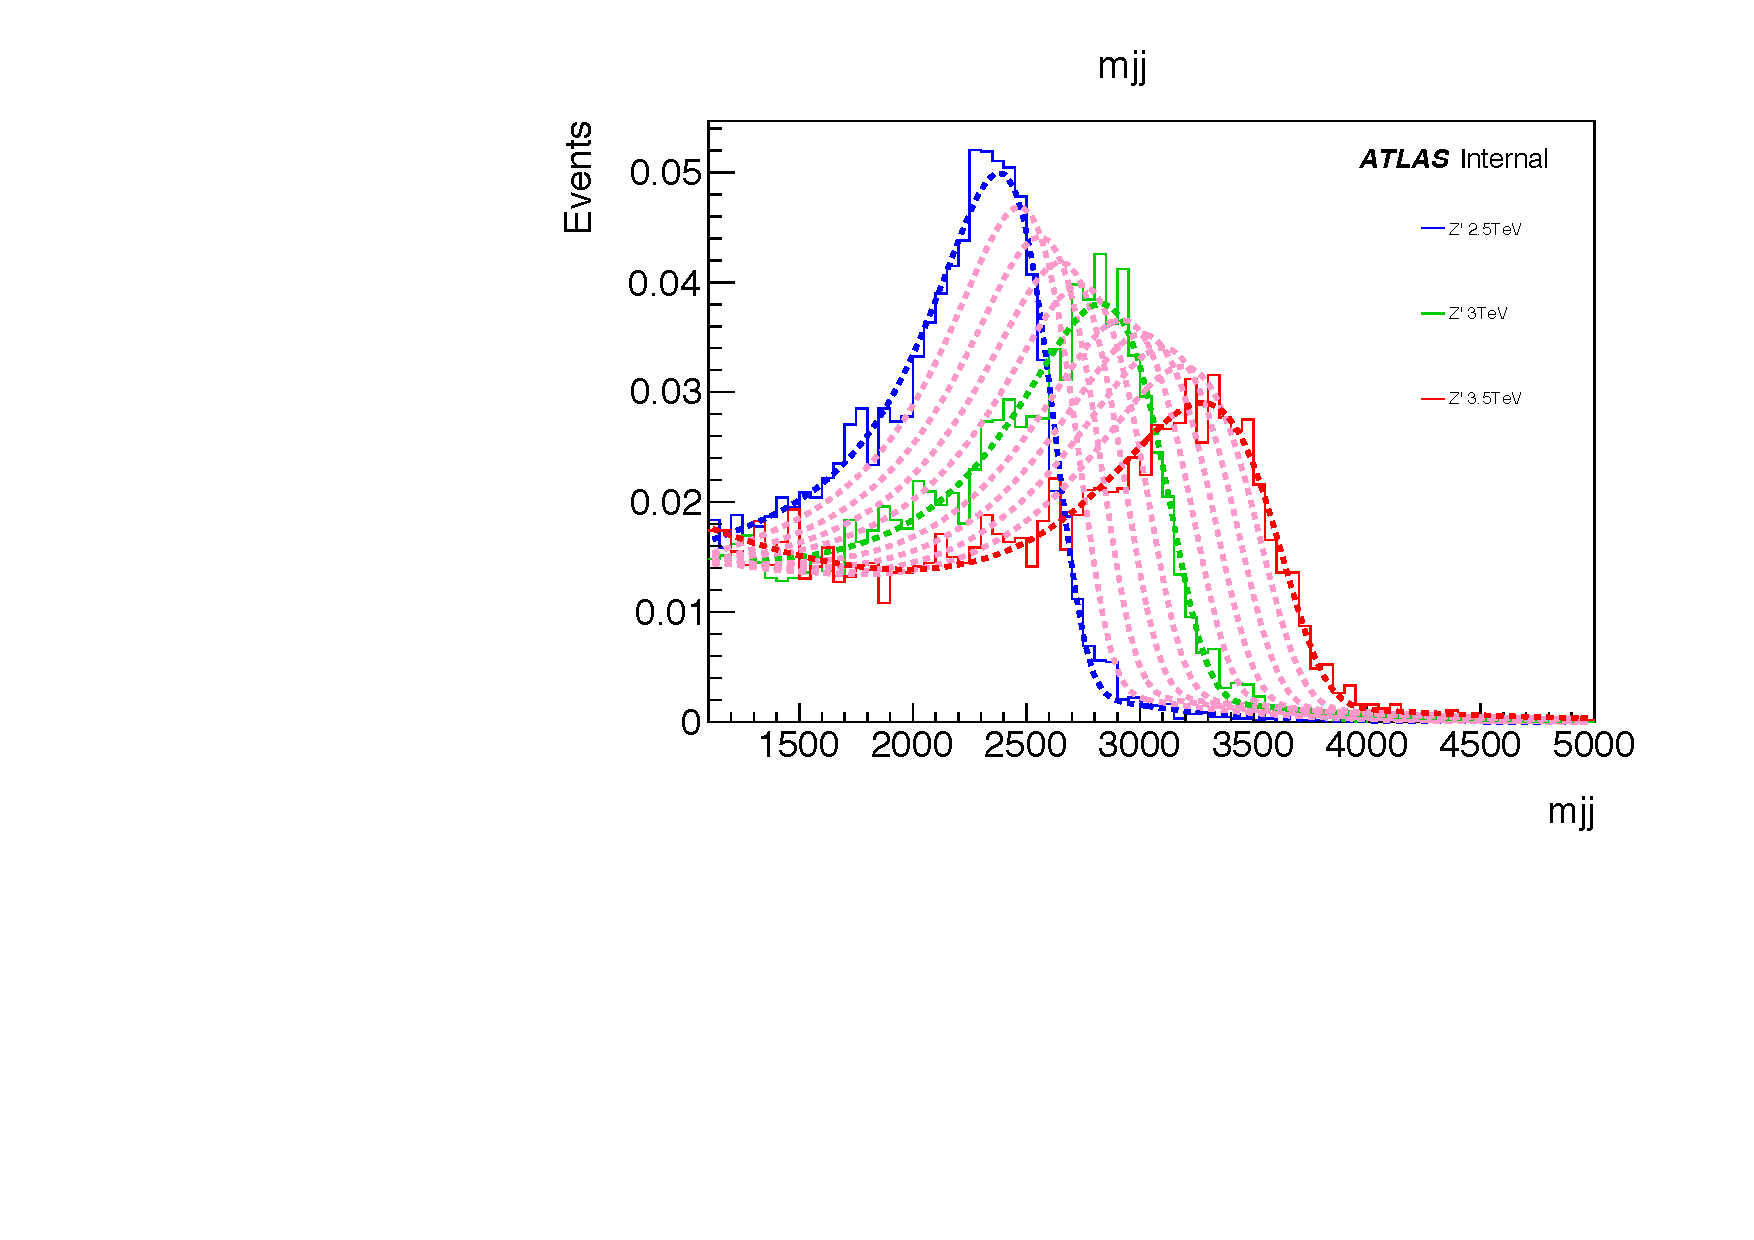
\includegraphics[width=0.48\textwidth]{figures/SWiFt/ZPrime_gSM0p50.pdf} }
	\caption{
		Signal morphing for some MC signals. The solid colored histograms are MC signal shapes and the dotted lines of the same color are fit to the MC shapes. The dotted pink curves are the morphed shapes.  
		\label{fig:morphing}}
\end{figure}

To stress test the morphing technique, tests were done where the a set of mass MC signal shapes were removed and the morphing was done with the remaining shapes. The results of this test is shown in figure~\ref{fig:morphingTest}, where in (a) integer MC q* shapes (2 \TeV\ , 3 \TeV\ , 4 \TeV\ , 5 \TeV\ , 6 \TeV\ ) are removed and morphing is done using the odd shapes only and in (b) fractional MC shapes (2.5 \TeV\ , 3.5 \TeV\ , 4.5 \TeV\ , 5.5 \TeV\ ) are removed and the even shapes are used for morphing. The technique recovers the shapes of the removed signals fairly well.  

\begin{figure}[!htb]
	\centering
	\subfigure[q* signals. Morphing with odd masses only.]{ 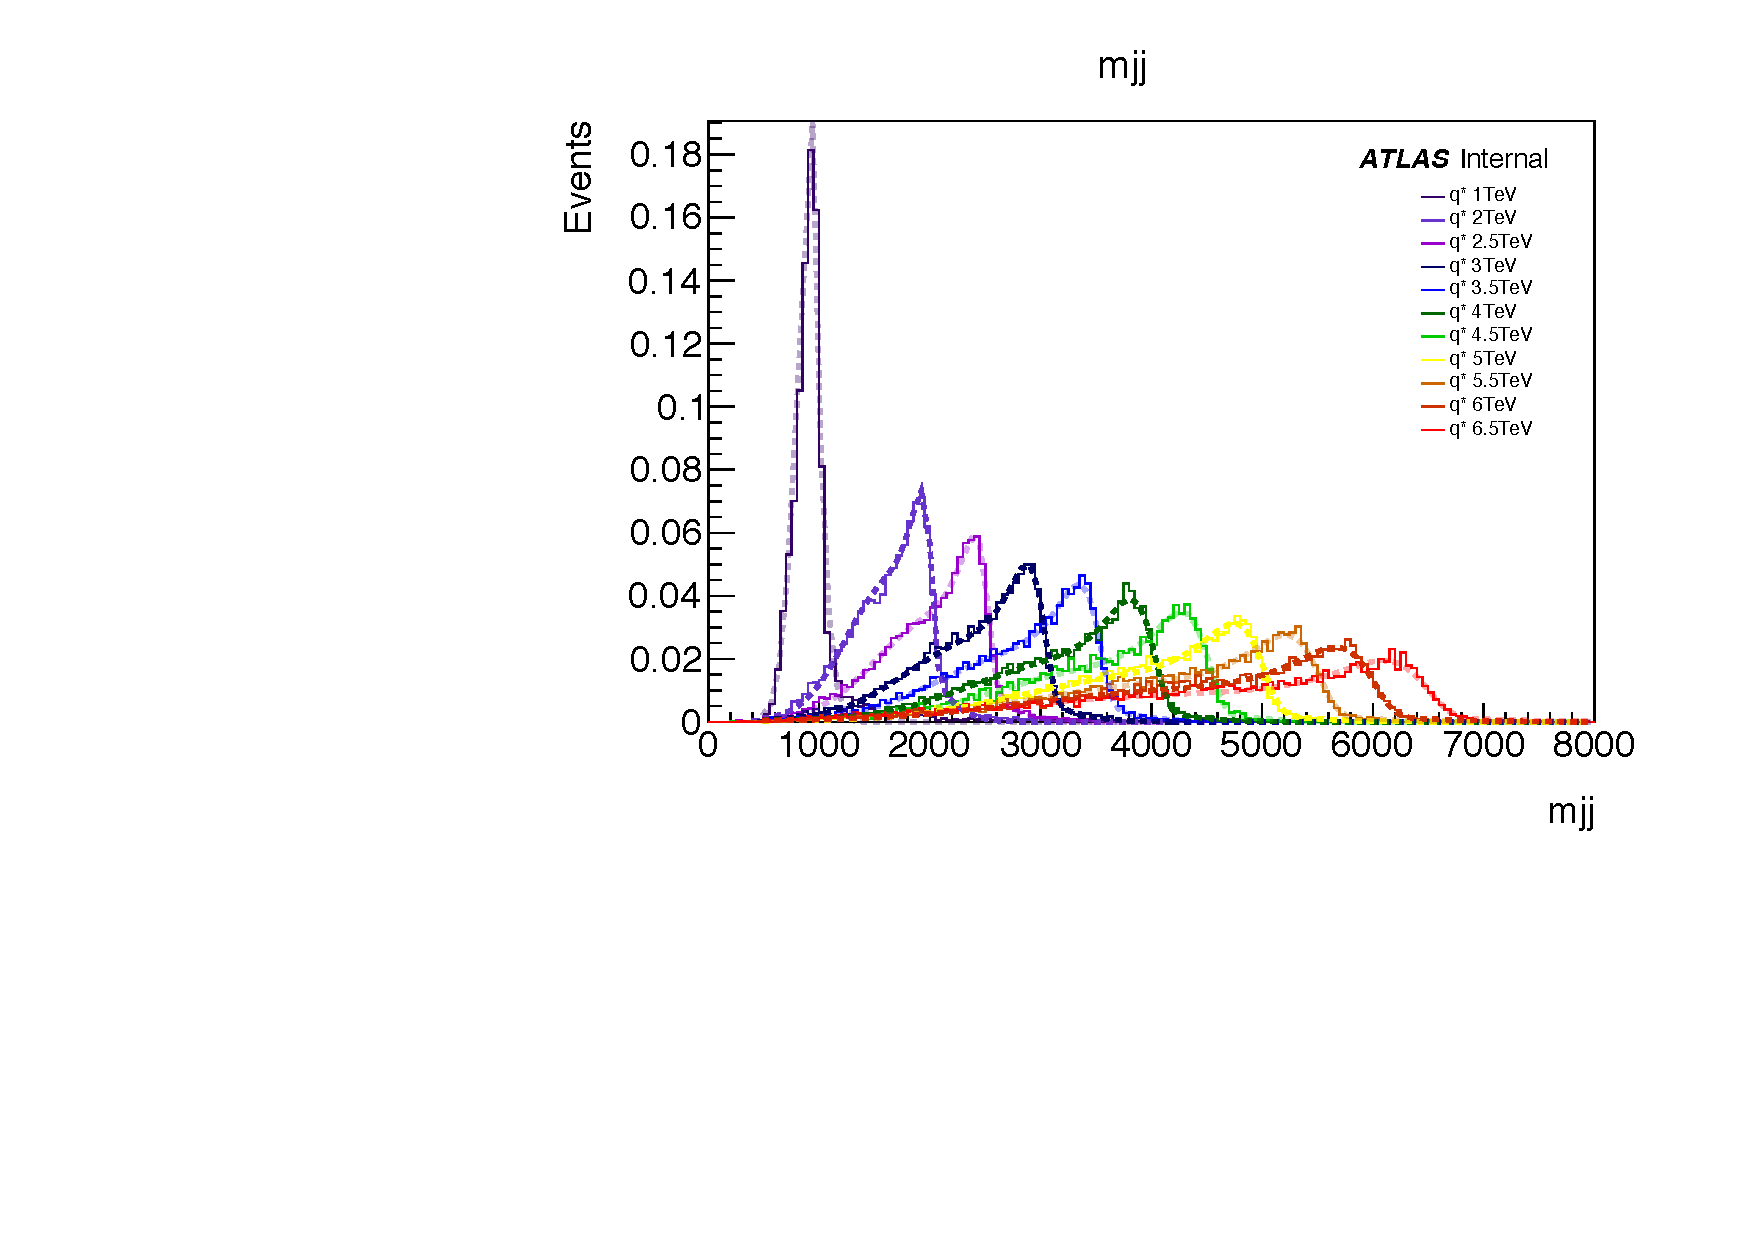
\includegraphics[width=0.48\textwidth]{figures/SWiFt/interpolateWorking_evenRemoved.pdf} }
	\subfigure[q* signals. Morphing with even masses only.]{ 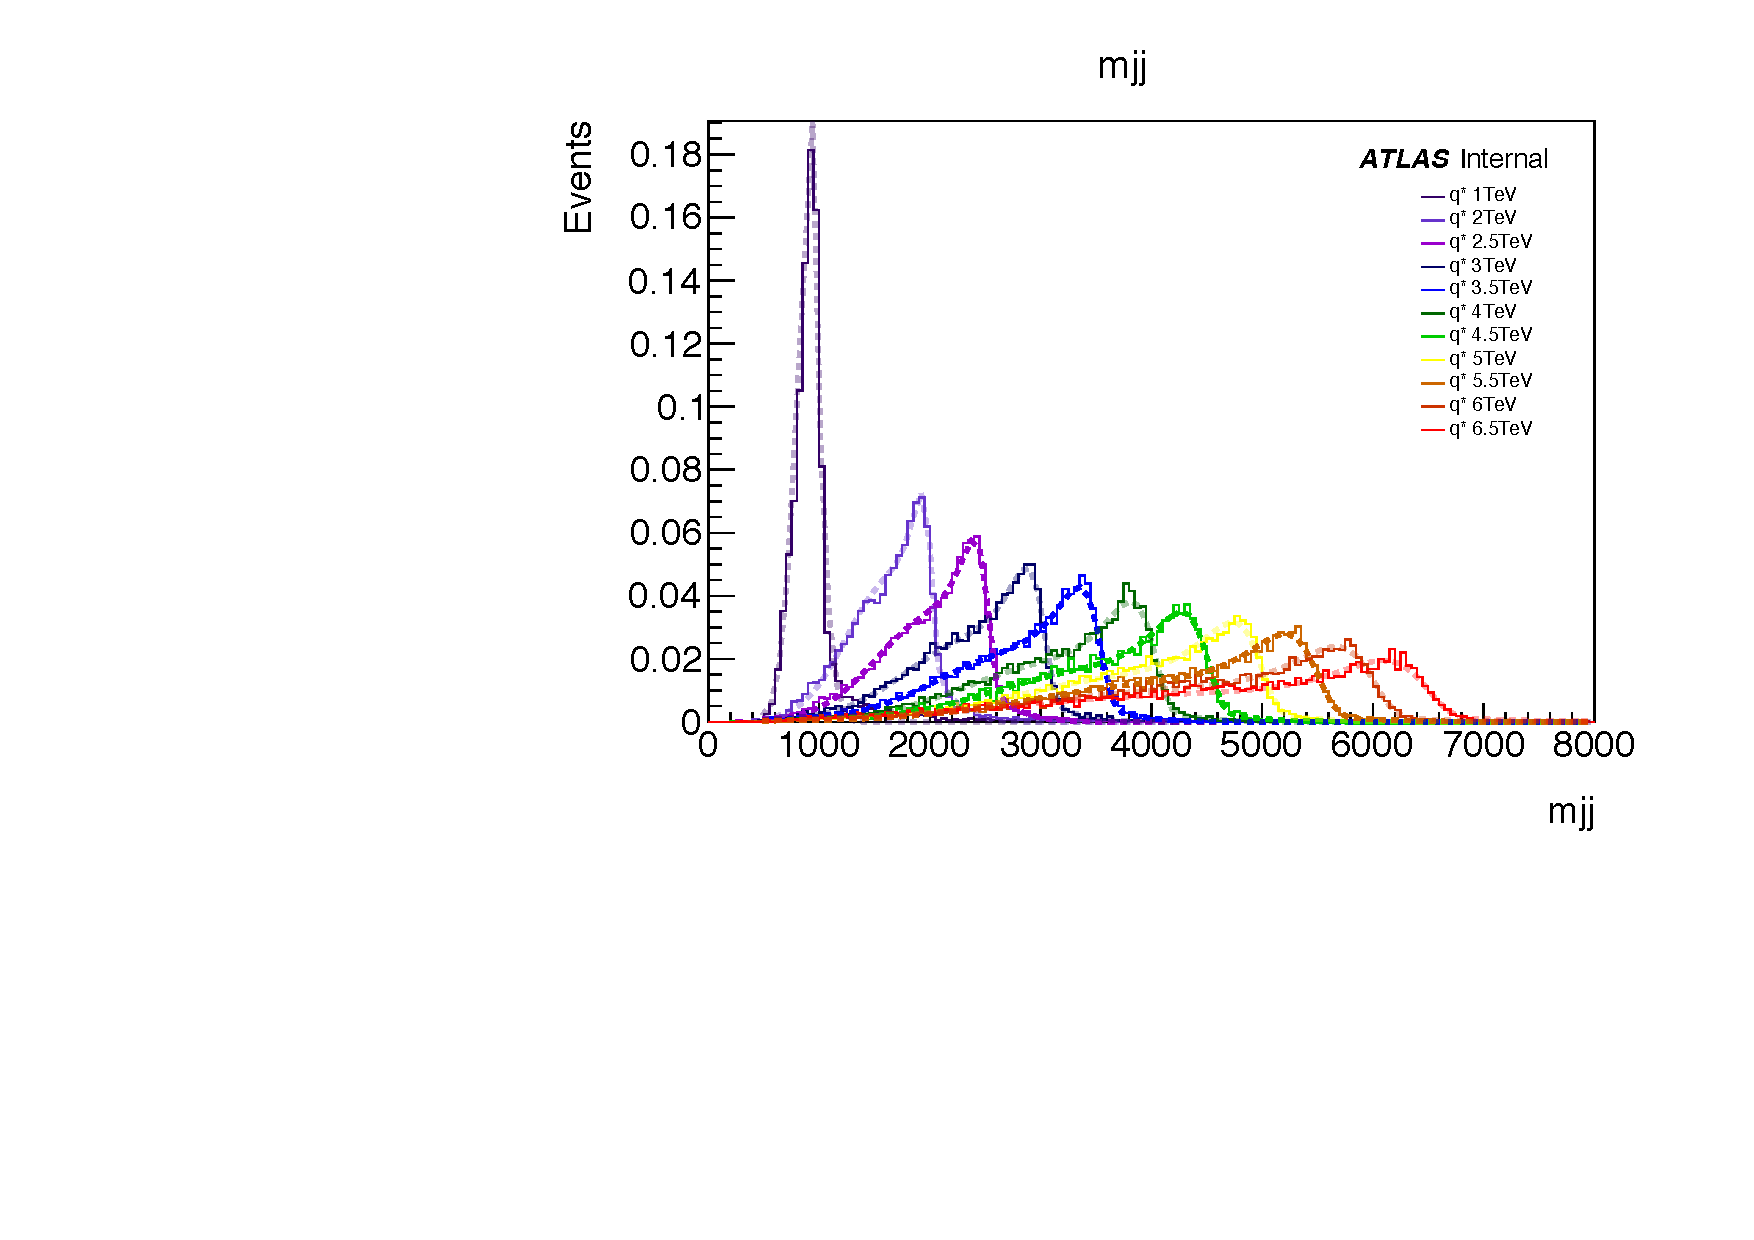
\includegraphics[width=0.48\textwidth]{figures/SWiFt/interpolateWorking_oddRemoved.pdf} }
	\caption{
		Signal morphing stress test. (a) Even mass signals are removed and morphing is done with odd masses only. (b) Odd mass signals are removed and morphing is done with even masses only. 
		\label{fig:morphingTest}}
\end{figure}  




\clearpage
%-------------------------------------------------------------------------------

%-------------------------------------------------------------------------------
\section{``Quark-Gluon'' Sample Selection}
\label{sec:QGselection}

It has been shown that the number of charged particles with transverse
momentum (\pT ) above 500\,MeV, \ntrk, associated with a jet can be used
to select samples which have an increased fraction of jets produced by
quarks (or gluons). Samples with enhanced fractions of quark or gluon
initiated jets can be created by using a selection based on the \ntrk\
as shown in Fig.~\ref{fig:jet_pt_quark_gluon}.
Ref.~\cite{ATL-PHYS-PUB-2017-009} also shows that the \Pythia8
generator~\cite{pythia8} using the A14 tune~\cite{A14tune} is in a good
agreement with the distribution of \ntrk\ found in data.


\begin{figure}[htb]
 \centering
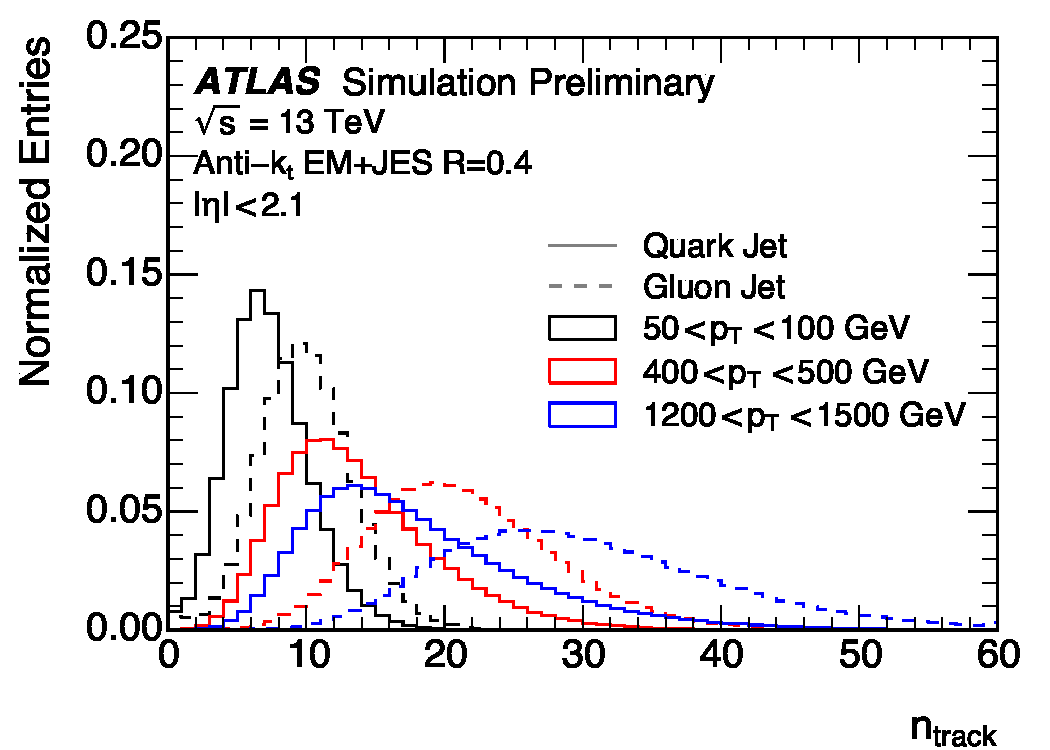
\includegraphics[width=0.75\textwidth]{figures/tagging/fig_01_ATL-PHYS-PUB-2017-009.pdf}
\caption{Distribution of the jet reconstructed track multiplicity (\ntrk ) in
 different pT ranges with the \Pythia~8 generator~\cite{pythia8} using
 the A14 tune~\cite{A14tune}, the NNPDF2.3 PDF
 set~\cite{Carrazza:2013axa}, and processes with a full simulation of the
 ATLAS detector. Jets must be fully within the tracking acceptance
 ($|\eta|<2.1$) and tracks are required to have $\pT > 500$\,MeV and pass
  quality criteria described in Ref.~\cite{ATL-PHYS-PUB-2017-009}. Figure
 from Ref.~\cite{ATL-PHYS-PUB-2017-009}. \label{fig:jet_pt_quark_gluon}}
\end{figure}

In Ref.~\cite{ATL-PHYS-PUB-2017-009}  the selection criteria for  an
enriched quark-initiated jet sample was chosen so that each \pT\ bin had
60\% quark-initiated purity. Applying this criteria to the high mass
dijet sample would lead to discontinuities in the mass spectrum that
would present difficulties to a resonance search. 

Using a selection criteria that is a linear function of the \( \ln \pT \) 
results in a smooth mass distribution and can be chosen to produce a uniform 
selection efficiency.  A jet is classed as being quark-initiated if \ntrk is less than
the threshold \nq and a gluon-initiated if \ntrk is greater than the threshold \ngluon  
\begin{align}
\ntrk & \le \nq \; \mbox{quark-initiated sample} \label{eq:QGselect} \\
\ntrk	  & \ge \ngluon \; \mbox{gluon-initiated sample} \nonumber
\end{align}
where   
\begin{equation}
n_{\mathrm{q(g)}} = {m \ln(\pT) + c}  \label{eq:nqg2}
\end{equation}
where $m$ and $c$ are constants chosen to provide suitable subsamples.

The constants $m$ and $c$ are found by finding the value of \ntrk\ 
that corresponds to a given efficiency for truth quark and gluon jets in 
\pT\ bins and fitting the results. The jet \pT\ bin edges are chosen to be 
400, 500, 650, 800, 1000, 1200, 1500, 2000, 3000, 6000\,\GeV. An example of the \ntrk cumulative 
distribution for truth quark and gluon jets satisfying $800 < \pT < 1000\,\GeV$ is shown in
Fig.~\ref{fig:ntrk_cumulative}.


\begin{figure}[htb]
 \centering
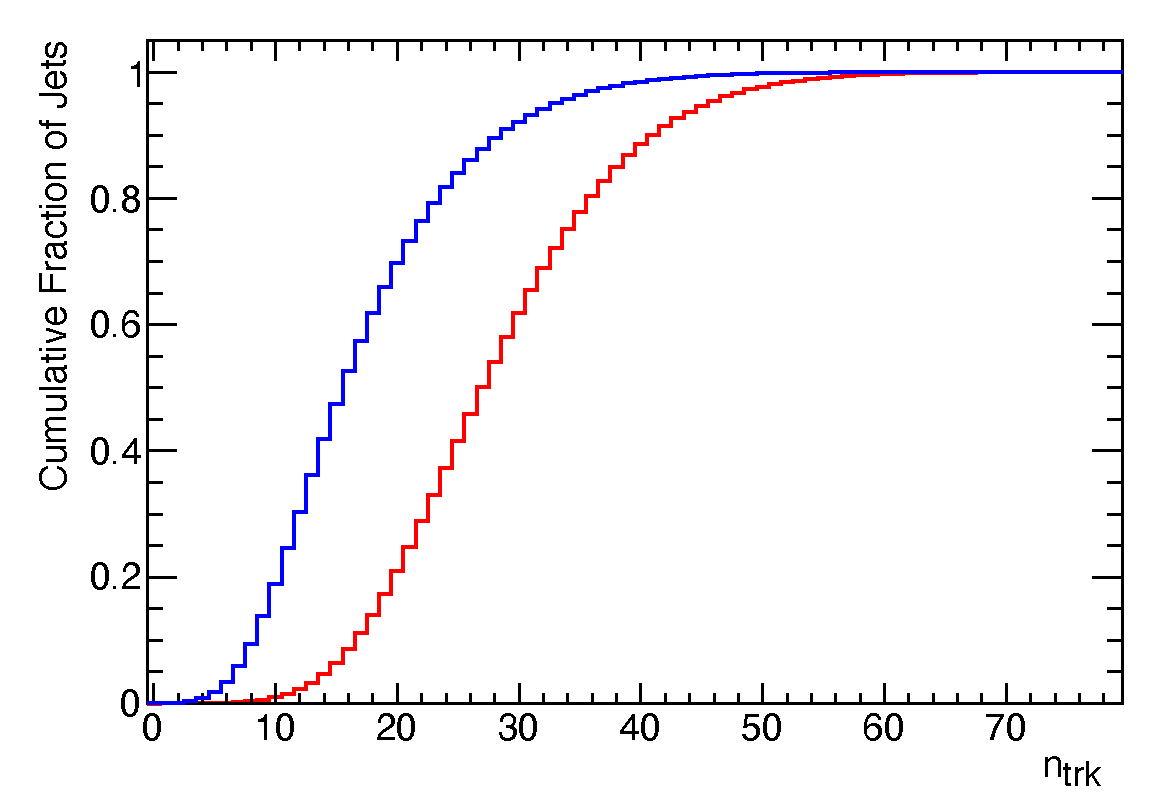
\includegraphics[width=0.75\textwidth]{figures/tagging/Cumulative_ntrk_distribution_4_800_1000GeV.pdf}
\caption{The cumulative distribution of \ntrk\ for truth quark (blue) and gluon (red) initiated jets 
satisfying $800 < \pT < 1000\,\GeV$.  \label{fig:ntrk_cumulative}}
\end{figure}


The constants for Eq.~\ref{eq:nqg2} are found for quark and gluon selection efficiencies from 
65\% to 95\% in 5\% steps. The plot of the value of \ntrk\ that satisfies the selection efficiencies 
of 70 and 80\% are shown in Fig.~\ref{fig:qg_selection_curves} along with the best fit using Eq.~\ref{eq:nqg2}.
The values of the constants for both quark and gluon selections are summarised in 
Tables~\ref{table:truthQuarkSelectionEfficiencies} and \ref{table:truthGluonSelectionEfficiencies}.

\begin{figure}[htb]
 \centering
  \subfigure[] {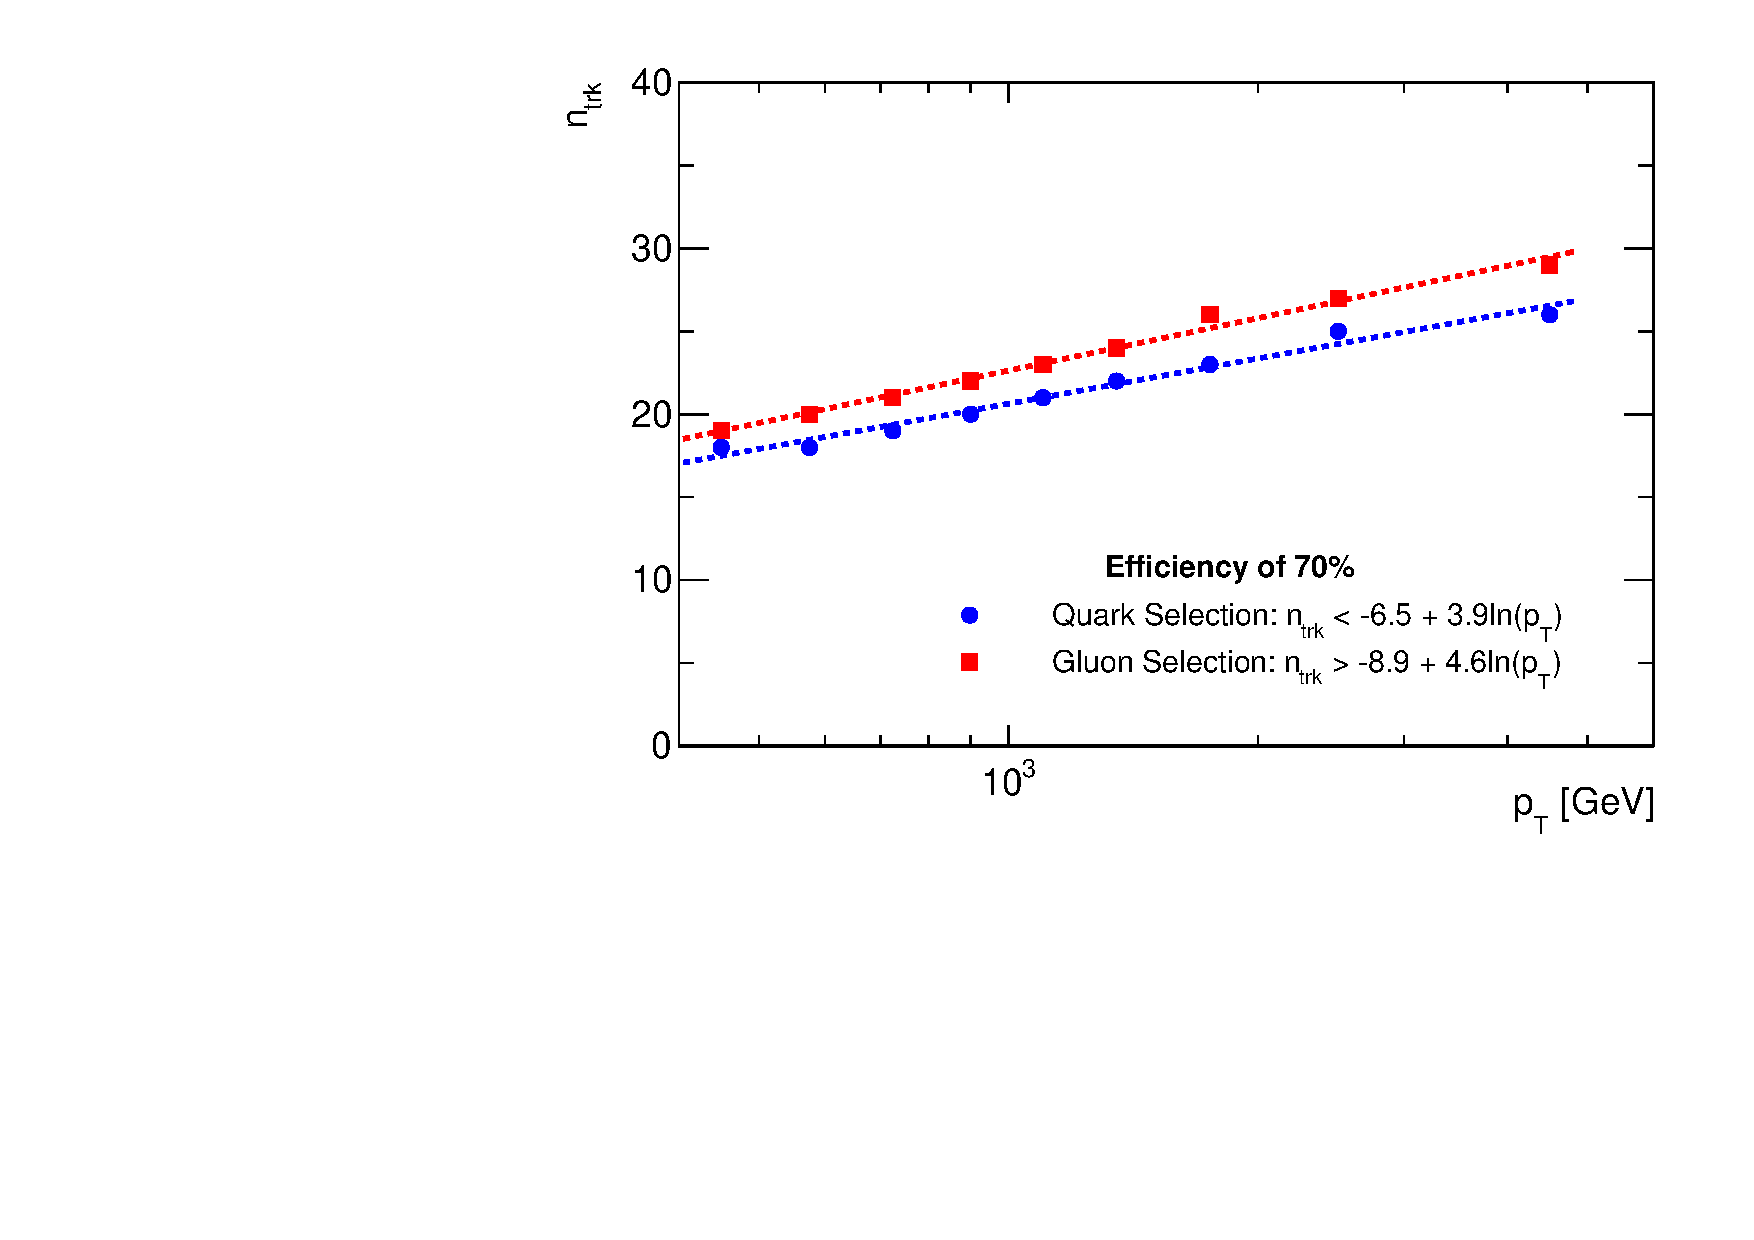
\includegraphics[width=0.495\textwidth]{figures/tagging/quark_selection_6}}
  \subfigure[] {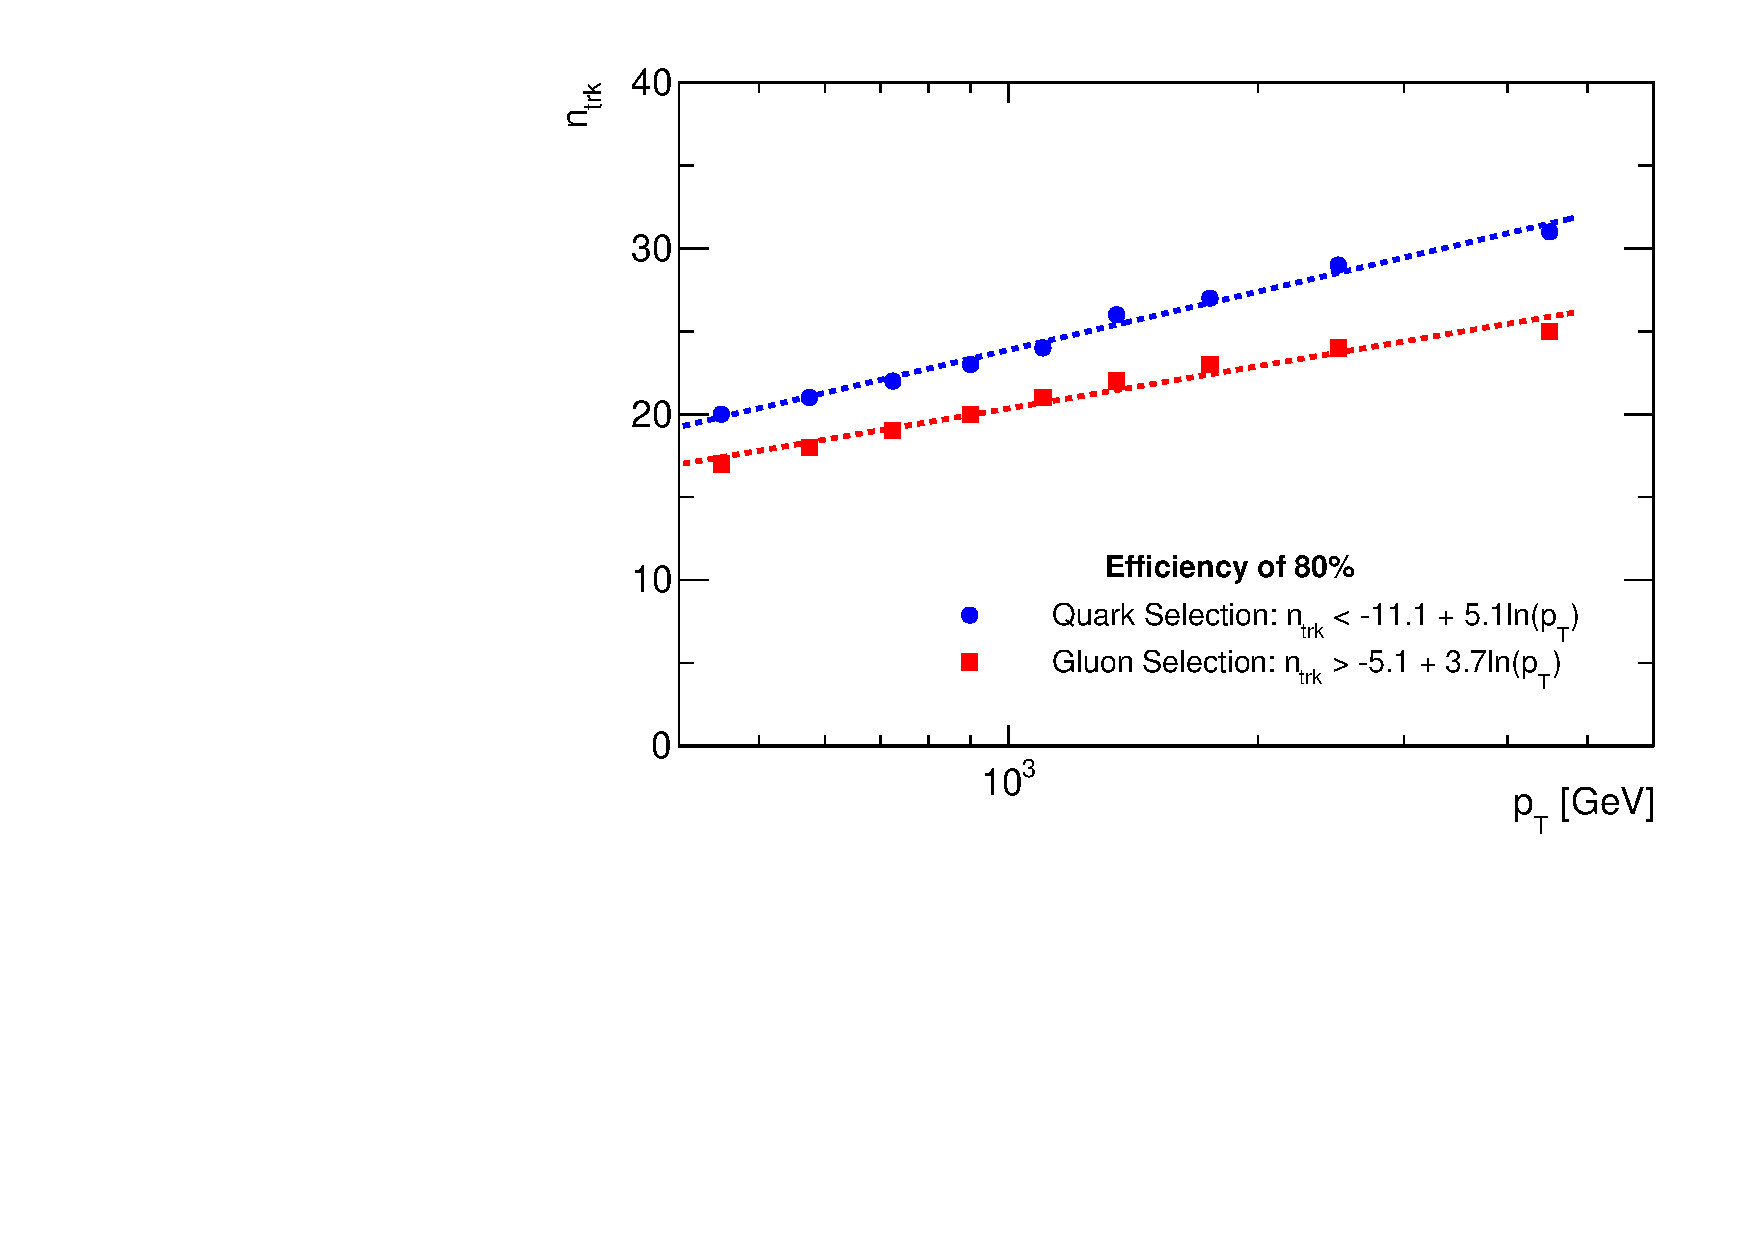
\includegraphics[width=0.495\textwidth]{figures/tagging/quark_selection_4}}

\caption{ The values of \ntrk\ for (a) 70\% and (b) 80\% quark (blue) and gluon (red) 
selection efficiencies in each \pT\ bin along with the best fit to Eq.~\ref{eq:nqg2}.
 \label{fig:qg_selection_curves}}
\end{figure}


\begin{table}[h]
	\centering 
		\caption{ Values of constants $m$ and $c$ from Eq.~\ref{eq:nqg2} such that $ \ntrk  \le \nq $ 
		for truth quark jets for a range of efficiencies  from 65 to 95\%. 
		\label{table:truthQuarkSelectionEfficiencies}
		}
	\begin{tabular}{SSSS}
	\toprule
\multicolumn{1}{c}{Truth-$q$ selection efficiency}   & \multicolumn{1}{c}{Truth-$g$ selection efficiency} &  \multicolumn{1}{c}{$c$}  &  \multicolumn{1}{c}{$m$} \\
\midrule 
0.95 & 0.73 & -20.0 & 7.7 \\
0.90 & 0.57 & -15.9 & 6.5 \\
0.85 & 0.45 & -13.1 & 5.6 \\
0.80 & 0.36 & -11.1 & 5.1 \\
0.75 & 0.28 & -9.1  & 4.5 \\
0.70 & 0.22 & -6.5  & 3.9 \\
0.65 & 0.18 & -4.4  & 3.5 \\
\bottomrule
\end{tabular}
\end{table}

\begin{table}[h]
	\centering 
		\caption{ Values of constants $m$ and $c$ from Eq.~\ref{eq:nqg2} such that $ \ntrk  \ge \ngluon $ 
		for truth quark jets for a range of efficiencies  from 65 to 95\%. 
		\label{table:truthGluonSelectionEfficiencies}
		}
	\begin{tabular}{SSSS}
	\toprule
\multicolumn{1}{c}{Truth-$g$ selection efficiency}   & \multicolumn{1}{c}{Truth-$q$ selection efficiency} &  \multicolumn{1}{c}{$c$}  &  \multicolumn{1}{c}{$m$} \\
\midrule 
0.95 & 0.59 & -3.9 & 2.7 \\
0.90 & 0.46 & -4.3 & 3.1 \\
0.85 & 0.39 & -5.4 & 3.5 \\
0.80 & 0.31 & -5.1 & 3.7 \\
0.75 & 0.27 & -7.3 & 4.2 \\
0.70 & 0.23 & -8.9 & 4.6 \\
0.65 & 0.20 & -8.0 & 4.6\\
\bottomrule
\end{tabular}
\end{table}


\subsection{Expected Signal Significance}

The dijet mass spectrum has a complex background with rapidly changing  fractions of events that originate 
from quark-quark, quark-gluon and gluon-gluon. The expected signal significance has been investigated using 
MC simulated  signals and background. The background is represented using the \QCD samples described 
in Section~\ref{qcdsamps}. 

\subsubsection{Signals that decay to quark-quark.}

The significance for signals that decay to a quark anti-quark pair are estimated using \Zprime\ models (Section~\ref{sec:Zprime}) using 
\begin{equation}
S = N_S \sum_i{ \dfrac{ f_{{qq}_i}\epsilon_{qQ}^2 + f_{{qg}_i}\epsilon_{qQ}\epsilon_{gQ} + f_{{gg}_i}\epsilon_{gQ}^2  } {\sqrt{ B_{{qq}_i}\epsilon_{qQ}^2 + B_{{qg}_i}\epsilon_{qQ}\epsilon_{gQ} + B_{{gg}_i}\epsilon_{gQ}^2  }}}
\end{equation}
where $N_S$ is the number of signal events, $f_{{qq}_i}$ is fraction of signal events that result in the two 
highest \pT\ jets that where initiated by quarks in bin $i$ ( $f_{{qg}_i}$ are quark-gluon jets, and $f_{{gg}_i}$ is two gluon jets), 
$\epsilon_{qQ}$ is the efficiency of a quark initiated jet passing the quark selection criteria, 
$\epsilon_{gQ}$ is the efficiency of a gluon initiated jet passing the quark selection criteria, 
and $B_{{xx}_i}$ is the expected number of background events with quark-quark, quark-gluon or gluon-gluon initiated jets. 


The significance is calculated for \Zprime's with masses ranging from 1500 to 4000\,\GeV and quark-jet selection 
efficiencies ranging from 30 to 90\%. The resulting significances are  in Fig.~\ref{fig:QuarkSignalSignificance}
and show that the significance decreases if any quark-selection is applied to the data. This is because
the data is dominated by quark-quark events and the selection reduces background and signal in similar amounts. 

\begin{figure}[htb]
 \centering
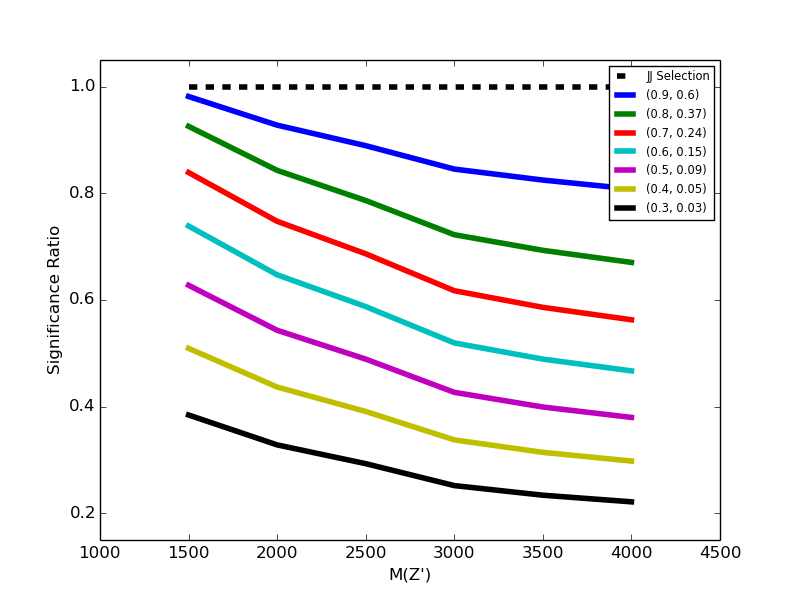
\includegraphics[width=0.75\textwidth]{figures/tagging/QuarkSignalSignificance.png}
\caption{ The significance for observing a \Zprime\ with masses from 1500 to 4000\,\GeV
for $\epsilon_{qQ}$ ranging from 90 to 30\% compared to the significance calculated with no quark selection applied. The key gives pairs of efficiencies ($\epsilon_{qQ}$, $\epsilon_{gQ}$).
  \label{fig:QuarkSignalSignificance}}
\end{figure}

\subsubsection{Signals that decay to gluon-gluon.}

The significance for signals that decay to a gluon-gluon pair are estimated using \Hprime\ models  using 
\begin{equation}
S = N_S \sum_i{ \dfrac{ f_{{qq}_i}\epsilon_{qG}^2 + f_{{qg}_i}\epsilon_{qG}\epsilon_{gG} + f_{{gg}_i}\epsilon_{gG}^2  } {\sqrt{ B_{{qq}_i}\epsilon_{qG}^2 + B_{{qg}_i}\epsilon_{qG}\epsilon_{gG} + B_{{gg}_i}\epsilon_{gG}^2  }}}
\end{equation}
where  
$\epsilon_{qG}$ is the efficiency of a quark initiated jet passing the gluon selection criteria, 
$\epsilon_{gG}$ is the efficiency of a gluon initiated jet passing the gluon selection criteria. 
The significance is calculated for \Hprime's with masses ranging from 2000 to 7000\,\GeV\ and quark-jet selection 
efficiencies ranging from 60 to 90\%. The resulting significances are  in Fig.~\ref{fig:GluonSignalSignificance}
and show that the significance increases from approximately 1.2 at 2\,TeV\ to 1.6 at 7\,\TeV\ with the greatest 
increases  occurring for gluon selection efficiency of 75\%. 

\begin{figure}[htb]
 \centering
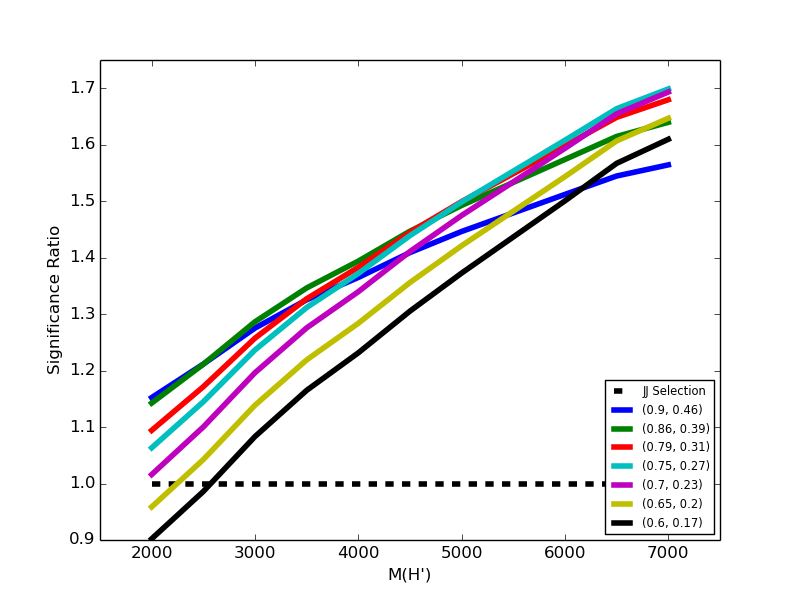
\includegraphics[width=0.75\textwidth]{figures/tagging/GluonSignalSignificance.png}
\caption{ The significance for observing a \Hprime\ with masses from 2000 to 7000\,\GeV\ 
for $\epsilon_{gG}$ ranging from 90 to 60\% compared to the significance calculated with no gluon selection applied. The key gives pairs of efficiencies ($\epsilon_{gG}$, $\epsilon_{qG}$).
  \label{fig:GluonSignalSignificance}}
\end{figure}


\subsubsection{Signals that decay to quark-gluon.}


The calculation of the significance for a quark-gluon signal such as an excited quark decay is much more complicated as 
both jets can satisfy both the quark and the gluon selection.  In this case we need to define three efficiencies that are exclusive for quark and gluon jets. They are 
\begin{itemize}
\item $\epsilon_{qQ}$ The probability that a quark initiated jet is identified only as a quark jet. 
\item $\epsilon_{qQG}$ The probability that a quark initiated jet is identified  as a quark and a gluon jet.
\item $\epsilon_{qG}$ The probability that a quark initiated jet is identified only as a gluon jet.  
\end{itemize}
where by construction $\epsilon_{qQ} + \epsilon_{qQG} + \epsilon_{qG} = 1$. A similar set of efficiencies are measured 
for gluon initiated jets. 
\begin{itemize}
\item $\epsilon_{gQ}$ The probability that a gluon initiated jet is identified only as a quark jet. 
\item $\epsilon_{gQG}$ The probability that a gluon initiated jet is identified  as a quark and a gluon jet.
\item $\epsilon_{gG}$ The probability that a gluon initiated jet is identified only as a gluon jet.  
\end{itemize}

The probability of truth quark-quark ($p_{qq}$), quark-gluon ($p_{qg}$) and gluon-gluon ($p_{gg}$) truth 
events of passing the selection criteria are given by 
\begin{align}
p_{qq} & = 2  \epsilon_{qQ}\epsilon_{qG} + \epsilon_{qQG}\left( \epsilon_{qQ} + \epsilon_{qG} \right)  + \epsilon_{qQG}\epsilon_{qQG} \\
p_{gg} & = 2  \epsilon_{gQ}\epsilon_{gG} + \epsilon_{gQG}\left( \epsilon_{gQ} + \epsilon_{gG} \right)  + \epsilon_{gQG}\epsilon_{gQG} \\
p_{qg} & = \epsilon_{qQ}\epsilon_{gG} + \epsilon_{gQ}\epsilon_{qG} + \epsilon_{qQG}\left( \epsilon_{gQ} + \epsilon_{gG} \right) 
+ \epsilon_{gQG}\left( \epsilon_{qQ} + \epsilon_{qG} \right) 
+ \epsilon_{gQG}\epsilon_{gQG}
\end{align}
and the significance is then given by 
\begin{equation}
S = N_S \sum_i{ \dfrac{ f_{{qq}_i} p_{qq} + f_{{qg}_i}p_{qg} + f_{{gg}_i}p_{gg}  } {\sqrt{ B_{{qq}_i}p_{qq} + B_{{qg}_i}p_{qg} + B_{{gg}_i}p_{gg}  }}}.
\end{equation}

Exploring selection efficiencies from 30 to 100\% for both quarks and gluons shows that no benefit 
is obtained by applying a quark selection. A small but significant improvement in significance is obtained 
if one of the two jets is required to pass a gluon selection. The resulting significances are  in Fig.~\ref{fig:QuarkGluonSignalSignificance}
and show that the significance increases by about 25\% at high masses (above 5\,\TeV ) with the greatest 
increases  occurring for gluon selection efficiency over 70\%. 


\begin{figure}[htb]
 \centering
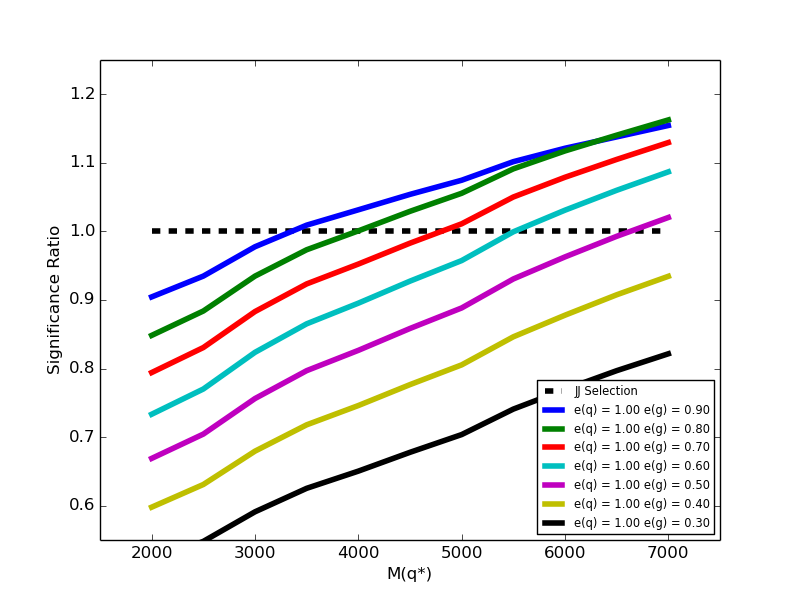
\includegraphics[width=0.75\textwidth]{figures/tagging/QuarkGluonSignalSignificance3.png}
\caption{ The significance for observing a \qstar\ with masses from 2000 to 7000\,\GeV\ 
for $\epsilon_{gG}$ ranging from 30 to 90\% compared to the significance calculated with no gluon selection applied. The key gives pairs of efficiencies ($\epsilon_{gG}$, $\epsilon_{qG}$).
  \label{fig:QuarkGluonSignalSignificance}}
\end{figure}


%\begin{equation}
%S = N_S \sum_i{ \dfrac{ f_{{qq}_i}\epsilon_{qG}^2 + f_{{qg}_i}\epsilon_{qG}\epsilon_{gG} + f_{{gg}_i}\epsilon_{gG}^2  } {\sqrt{ B_{{qq}_i}\epsilon_{qG}^2 + B_{{qg}_i}\epsilon_{qG}\epsilon_{gG} + B_{{gg}_i}\epsilon_{gG}^2  }}}
%\end{equation}
%
%
%
%Two alternative
%selection criteria have been investigated, one based on that used in
%Ref.~\cite{ATL-PHYS-PUB-2017-009} and a simple linear alternative. A jet
%is classed as being quark-initiated if \ntrk is less than the threshold
%\nqg\ (Eq.~\ref{eq:QGselect}):

%These selection criteria are applied to the two leading jets to separate dijet events into three samples:
%where both jets are more likely to be quark-initiated, \QQ,  where both jets are more likely to
%be gluon-initiated, \GG, and where we have one of each, \QG.
%Simulated background events are separated into sub-samples based on the selection criteria given in
%Eqs.~\ref{eq:nqg1} and \ref{eq:nqg2} and are shown in Fig.~\ref{fig:pythia_qg_selection}. It is clear that
%the selection using Eq.~\ref{eq:nqg1} (Fig.~\ref{fig:pythia_qg_selection} a) produces more complex background shapes
%than those Eq.~\ref{eq:nqg2} (Fig.~\ref{fig:pythia_qg_selection} b). Since the selection using  Eq.~\ref{eq:nqg2} will
%be much easier to fit it will be used for initial toy-MC studies of limit setting. Alternative selections using Eq.~\ref{eq:nqg2} are produced for comparison, "selection 1" with m = 0.02, c = 0, and "selection 4" with m = 0.01, c = 15.

%
%
%Figure~\ref{fig:QG_qstar_4tev} shows the selection applied to the mass distribution of a 4\,TeV \qstar . The  
%\QQ sample is more peaked and has a smaller tail than the \QG\ distribution which has a similar shape to the complete signal. The \GG\ sample of high multiplicity jets has a very small peak and is dominated by the tail.
%
%\begin{figure}[htb]
% \centering
%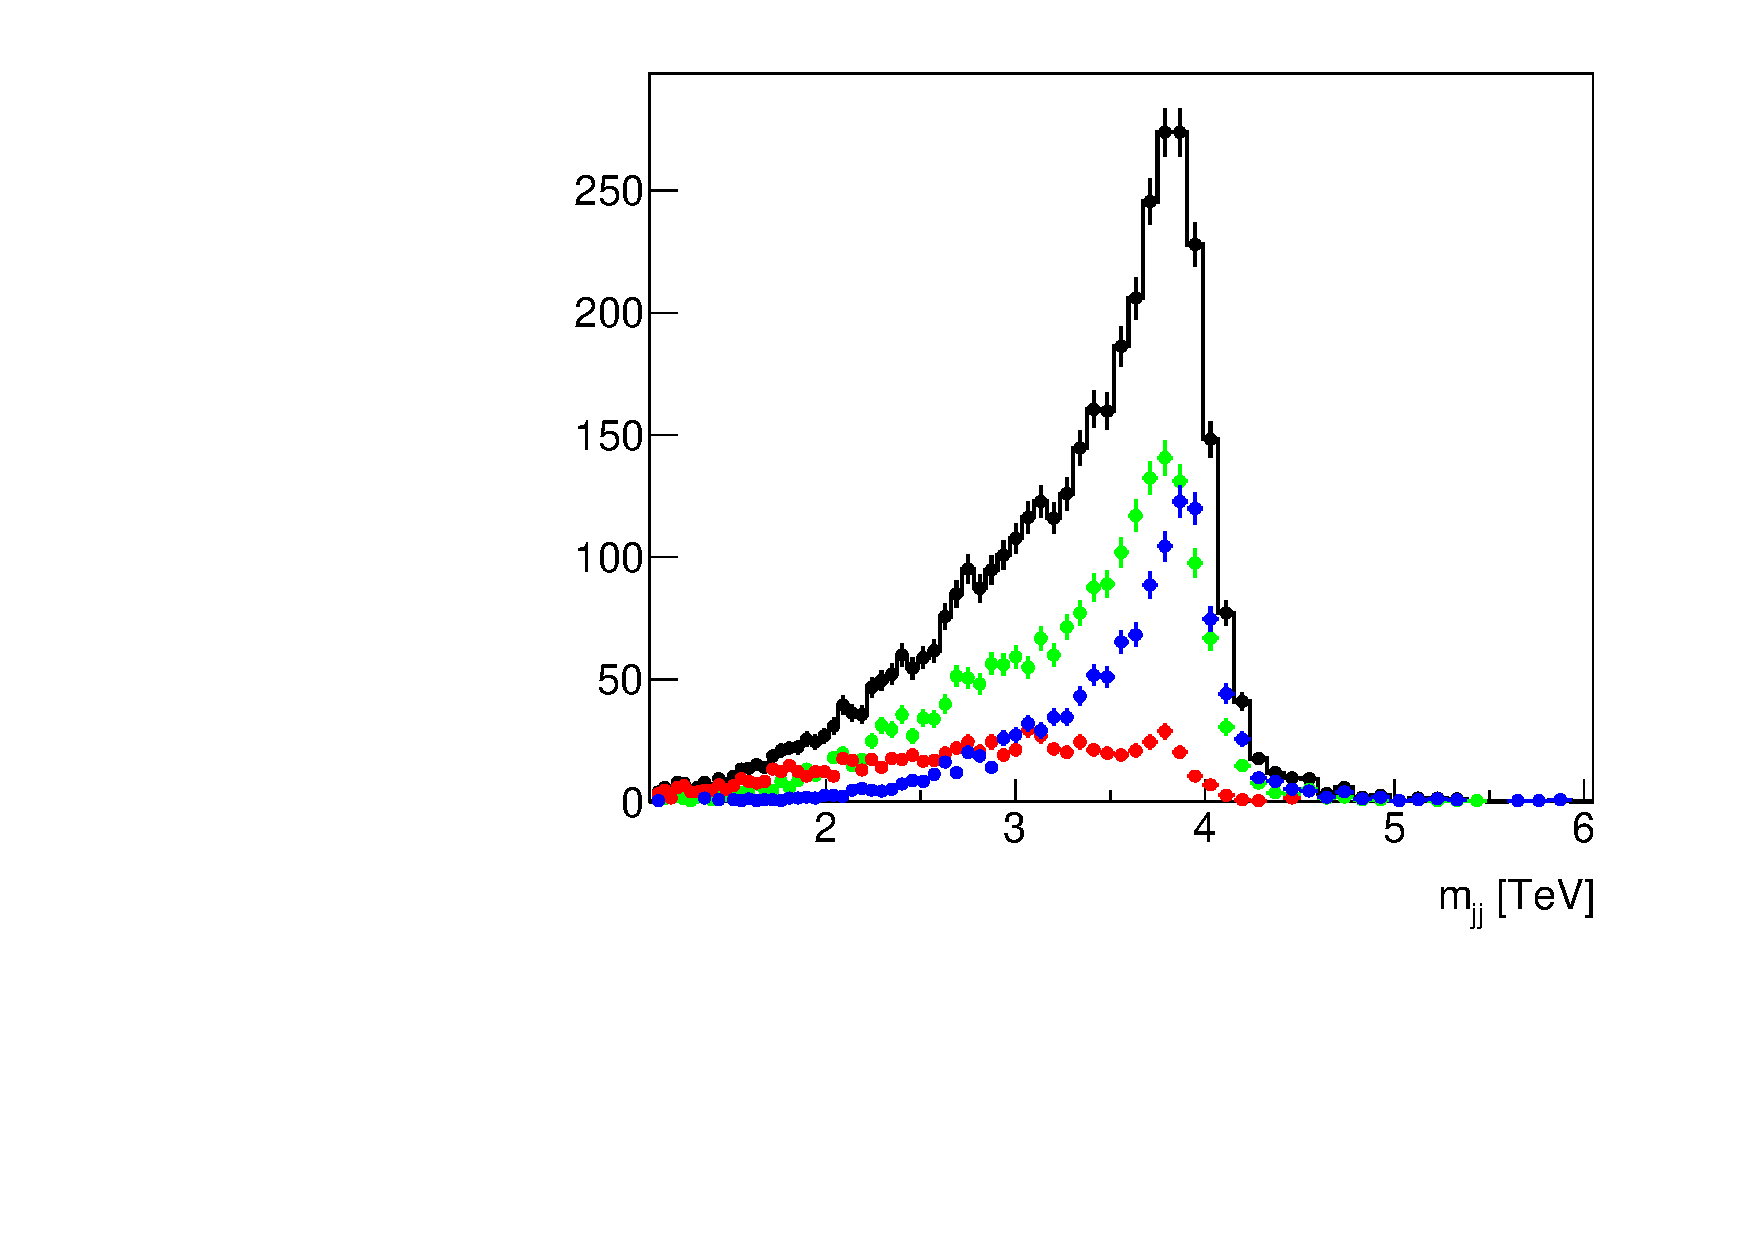
\includegraphics[width=0.75\textwidth]{figures/tagging/QG_qstar_4tev.pdf}
%\caption{Simulated 4\,TeV \qstar\ sample seperated into \QQ\ (blue) , \QG\ (green) and \GG\ (red) 
%sub-samples.  \label{fig:QG_qstar_4tev}}
%\end{figure}
%
%\clearpage
%\subsection{Signal Fractions Quark-Gluon selection}
%
%The fraction of \qstar\ signal events is measured for masses from 1\,TeV to 7.0\,TeV and are given in Table~\ref{table:qstar_fractions}. The low fraction of \QQ\ events at masses from 1 to 3\,TeV suggest that
%further optimisation of the selection criteria are required.  
%
%\begin{table}[h]
%	\centering 
%		\caption{The fraction of \qstar\ MC events in the \QQ, \QG, and \GG\ sub-samples for various masses. 
%		\label{table:qstar_fractions}}
%	\begin{tabular}{SSSS}
%	\toprule
%\qstar\ Mass (TeV) & \multicolumn{1}{c}{\QQ\ Fraction} &  \multicolumn{1}{c}{\QG\ Fraction}  &  \multicolumn{1}{c}{\GG\ Fraction} \\
%\midrule 
%1.0	&	0.06 &	0.31 &	0.63\\
%2.0	&	0.04 &	0.37 &	0.59\\
%2.5	&	0.09 &	0.45 & 	0.46\\
%3.0	&	0.15 &	0.51 &	0.35\\
%3.5	&	0.22 &	0.53 &	0.25\\
%4.0	&	0.30 &	0.51 &	0.19\\
%4.5	&	0.37 &	0.48 &	0.15\\
%5.0	&	0.44 &	0.44 &	0.12\\
%5.5	&	0.49 &	0.41 &	0.10\\
%6.0	&	0.53 &	0.37 &	0.09\\
%6.5	&	0.56 &	0.35 &	0.09\\
%7.0	&	0.57 &	0.33 &	0.10\\
%\bottomrule
%\end{tabular}
%\end{table}
%
%
%\begin{figure}[htb]
% \centering
%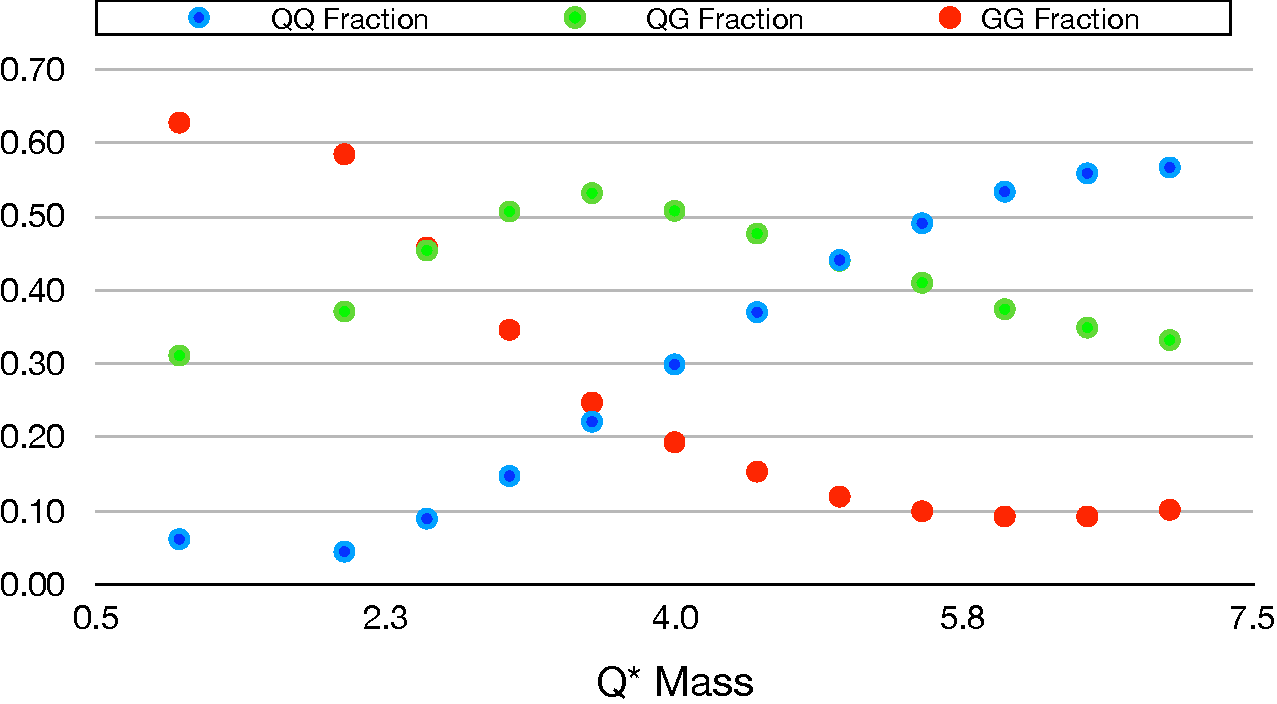
\includegraphics[width=0.75\textwidth]{figures/tagging/QStarEfficincies.pdf}
%\caption{The fraction of \qstar\ MC events in the \QQ, \QG, and \GG\ sub-samples for various masses.   \label{fig:QStarEfficincies}}
%\end{figure}
%
%
%
%\subsection{Signal Morphing with Quark-Gluon selection}
%
%Signal morphing (Sec.\ref{sec:SwiftMorphing}) is applied to the \qstar\ signal subsamples. The MC signal 
%sub-samples for \QQ\ and \QG\ are fit to a Gaussian + reverse Landau function, a parameterization that has 
%one normalization  and five shape parameters. The parameters are interpolated as a function of mass using cubic splines.
%%\textit{ \color{red} The \GG\ subsamples have not been morphed at this time.} 
%

\clearpage
%-------------------------------------------------------------------------------

%-------------------------------------------------------------------------------
\section{``Quark-Gluon'' Resonance Search Sensitivity}
\label{sec:QGselection}

As shown in Section~\ref{sec:ExpectedSig} we expect to see significant improvements in the limits for 
particles that decay to gluon-gluon and possible improvements in searches that involve a quark-gluon 
final state. In both cases the optimal search is by selecting only on the gluon initiated jets with a 
nominal efficiency of 75\%.  

The choice of operating pint will be confirmed by using pseudo-data (Section~\ref{sec:pseudo}) to test 
the selection efficiency by 
running the fitting and limit setting procedure of samples generated with selection efficiencies ranging from 
65 to 90\% in 5\% steps. 

\subsection{Signals that decay to gluon-gluon.}


The pseudo-data tests of the significance of gluon-gluon searches are studied using  \Hprime\ models as the signal. 
Each pseudo-data sample is fitted with SWiFt to estimate the background and then passed through \texttt{HistFitter}. 
For the initial estimation of the effectiveness of the selection we only include statistical uncertainties, 
the uncertainty on the integrated luminosity and an additional uniform 5\% uncertainty that is an initial 
guess of the magnitude of the uncertainty due to the gluon selection.  These results are compared to limits 
produced using pseudo-data created assuming no gluon selection has been applied. 

The resulting expected limits are plotted in Fig.~\ref{fig:GluonSignalSignificancePD}  and show a clear 
improvement in the expected limits for all the investigated gluon selection criteria. If we take the 
ratio of the expected cross section limits with gluon selection applied divided by the limits with no 
selection applied (Fig.~\ref{fig:GluonSignalSignificanceRatio}) shows that there is no obvious optimal
selection criteria. We have chosen 75\% as it performs well at masses above 4\,\TeV\ while we finalise 
the estimation of systematic uncertainties. 


\begin{figure}[htb]
 \centering
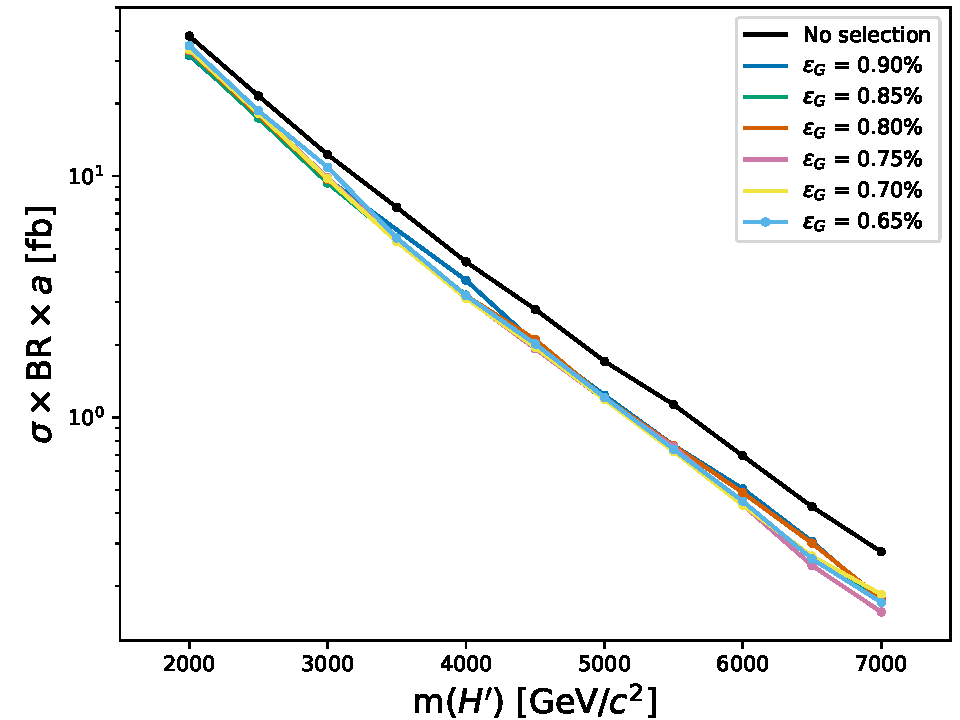
\includegraphics[width=0.75\textwidth]{figures/significance/Limits_GG_All.pdf}
\caption{ The expected cross section limits for a \Hprime\ with masses from 2000 to 7000\,\GeV\ 
for $\epsilon_{gG}$ ranging from 65 to 90\% compared to the significance calculated with 
   no gluon selection applied.
  \label{fig:GluonSignalSignificancePD}}
\end{figure}

\begin{figure}[htb]
 \centering
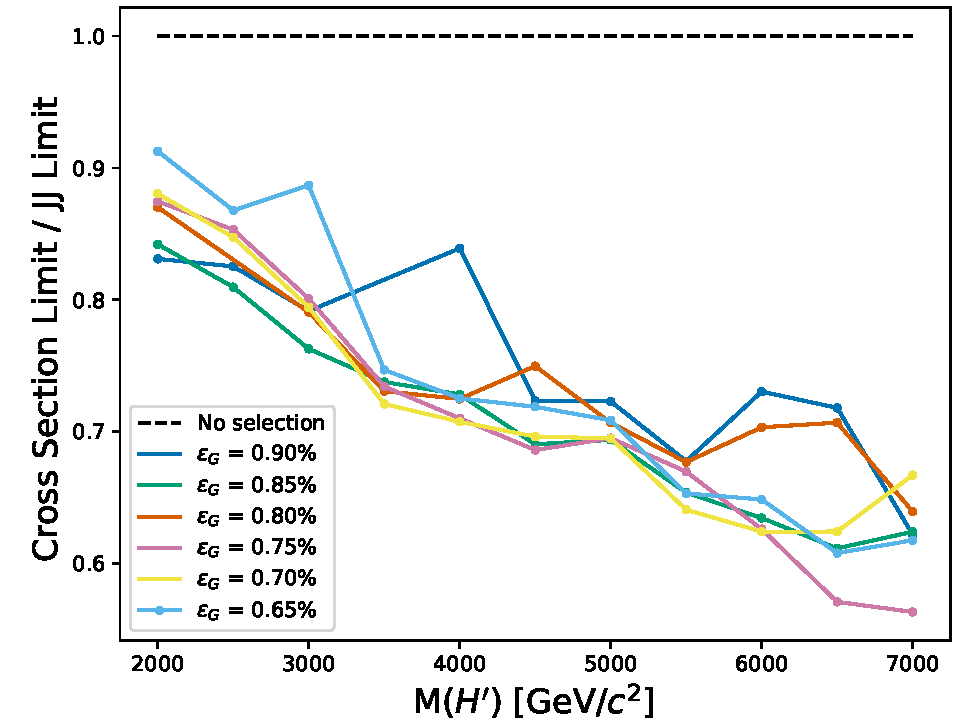
\includegraphics[width=0.75\textwidth]{figures/significance/Ratio_GG_All.pdf}
\caption{ The ratio of the expected cross section limits with gluon selection applied divided by the limits with no selection applied for a \Hprime\ with masses from 2000 to 7000\,\GeV. \label{fig:GluonSignalSignificanceRatio}}
\end{figure}


\subsection{Signals that decay to quark-gluon.}

The same procedure is applied for the significance of quark-gluon searches except that a \qstar\ is used for the signal. 
The resulting expected limits are plotted in Fig.~\ref{fig:QuarkGluonSignalSignificancePD}  and show a small 
improvement in the expected limits for all the investigated gluon selection criteria. If we take the 
ratio of the expected cross section limits with gluon selection applied divided by the limits with no 
selection applied (Fig.~\ref{fig:QuarkGluonSignalSignificanceRatio}) shows that there is no obvious optimal
selection criteria. We have chosen 75\% as it performs well at masses above 4\,\TeV\ while we finalise 
the estimation of systematic uncertainties. 



\begin{figure}[htb]
 \centering
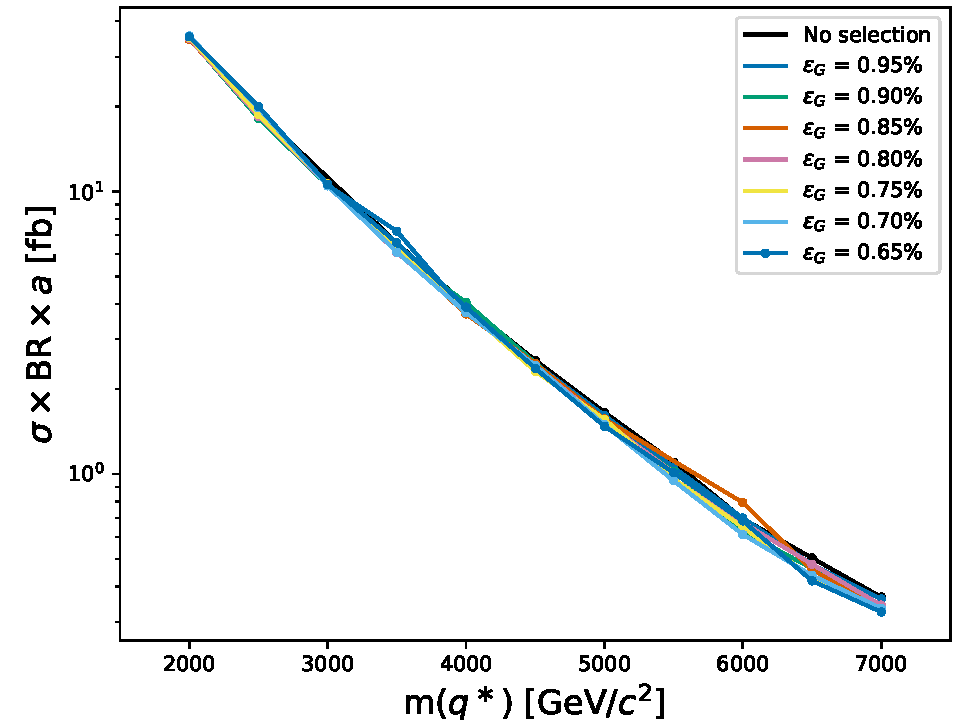
\includegraphics[width=0.75\textwidth]{figures/significance/Limits_QG_All.pdf}
\caption{ The expected cross section limits for a \qstar\ with masses from 2000 to 7000\,\GeV\ 
for $\epsilon_{gG}$ ranging from 65 to 90\% compared to the significance calculated with 
   no gluon selection applied.
  \label{fig:QuarkGluonSignalSignificancePD}}
\end{figure}

\begin{figure}[htb]
 \centering
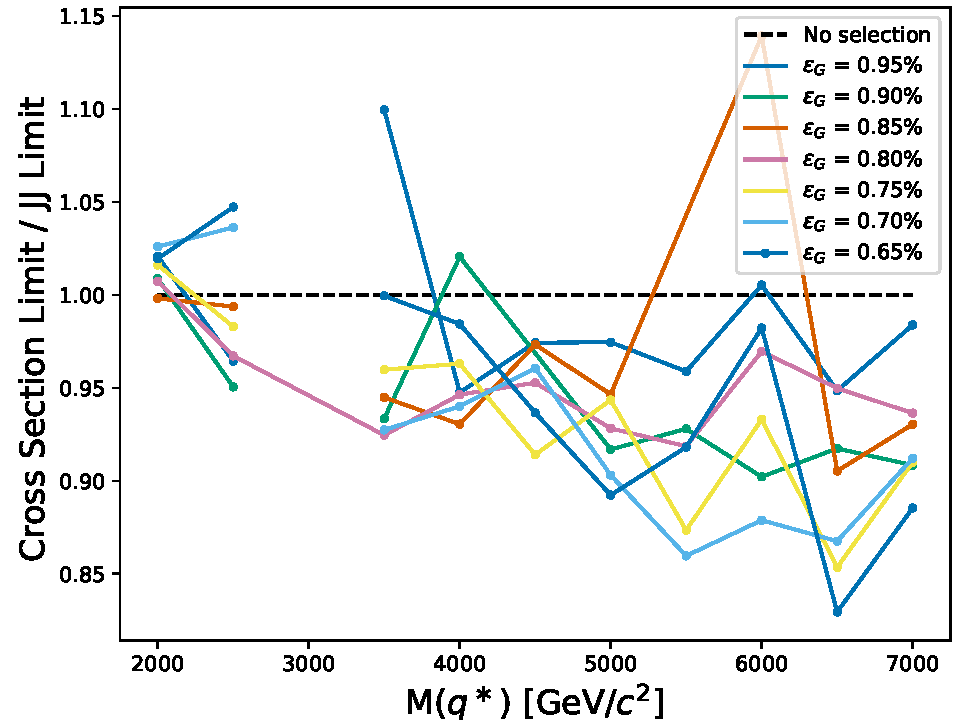
\includegraphics[width=0.75\textwidth]{figures/significance/Ratio_QG_All.pdf}
\caption{ The ratio of the expected cross section limits with gluon selection applied divided by the limits with no selection applied for a \qstar\ with masses from 2000 to 7000\,\GeV. \label{fig:QuarkGluonSignalSignificanceRatio}}
\end{figure}


%Ratio_GG_All.pdf


%\begin{figure}[p]
% \centering
%
% \subfigure[JJ] {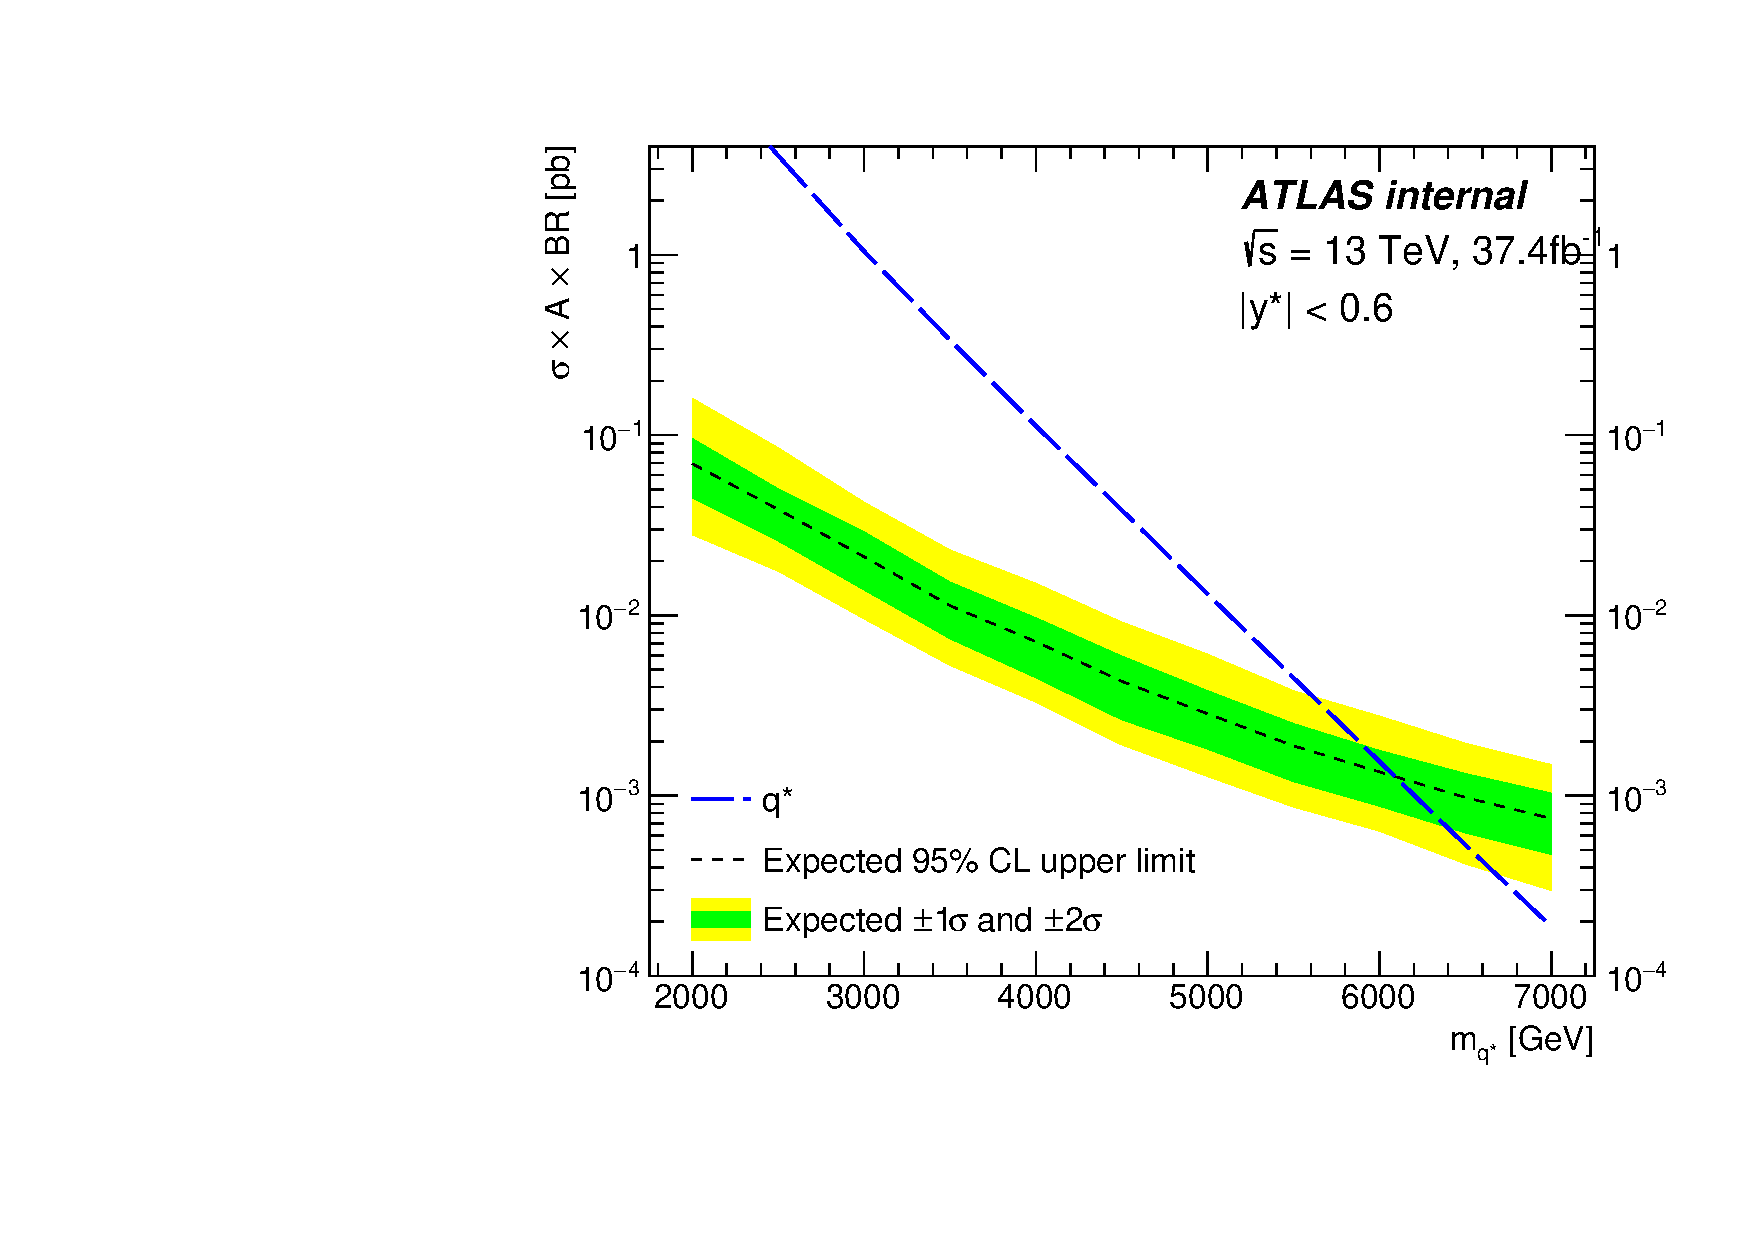
\includegraphics[width=0.475\textwidth] {figures/tagging/brazil-qStarMorphSingleJJUpdated.pdf}}
% \subfigure[\QQ\ \& \QG] {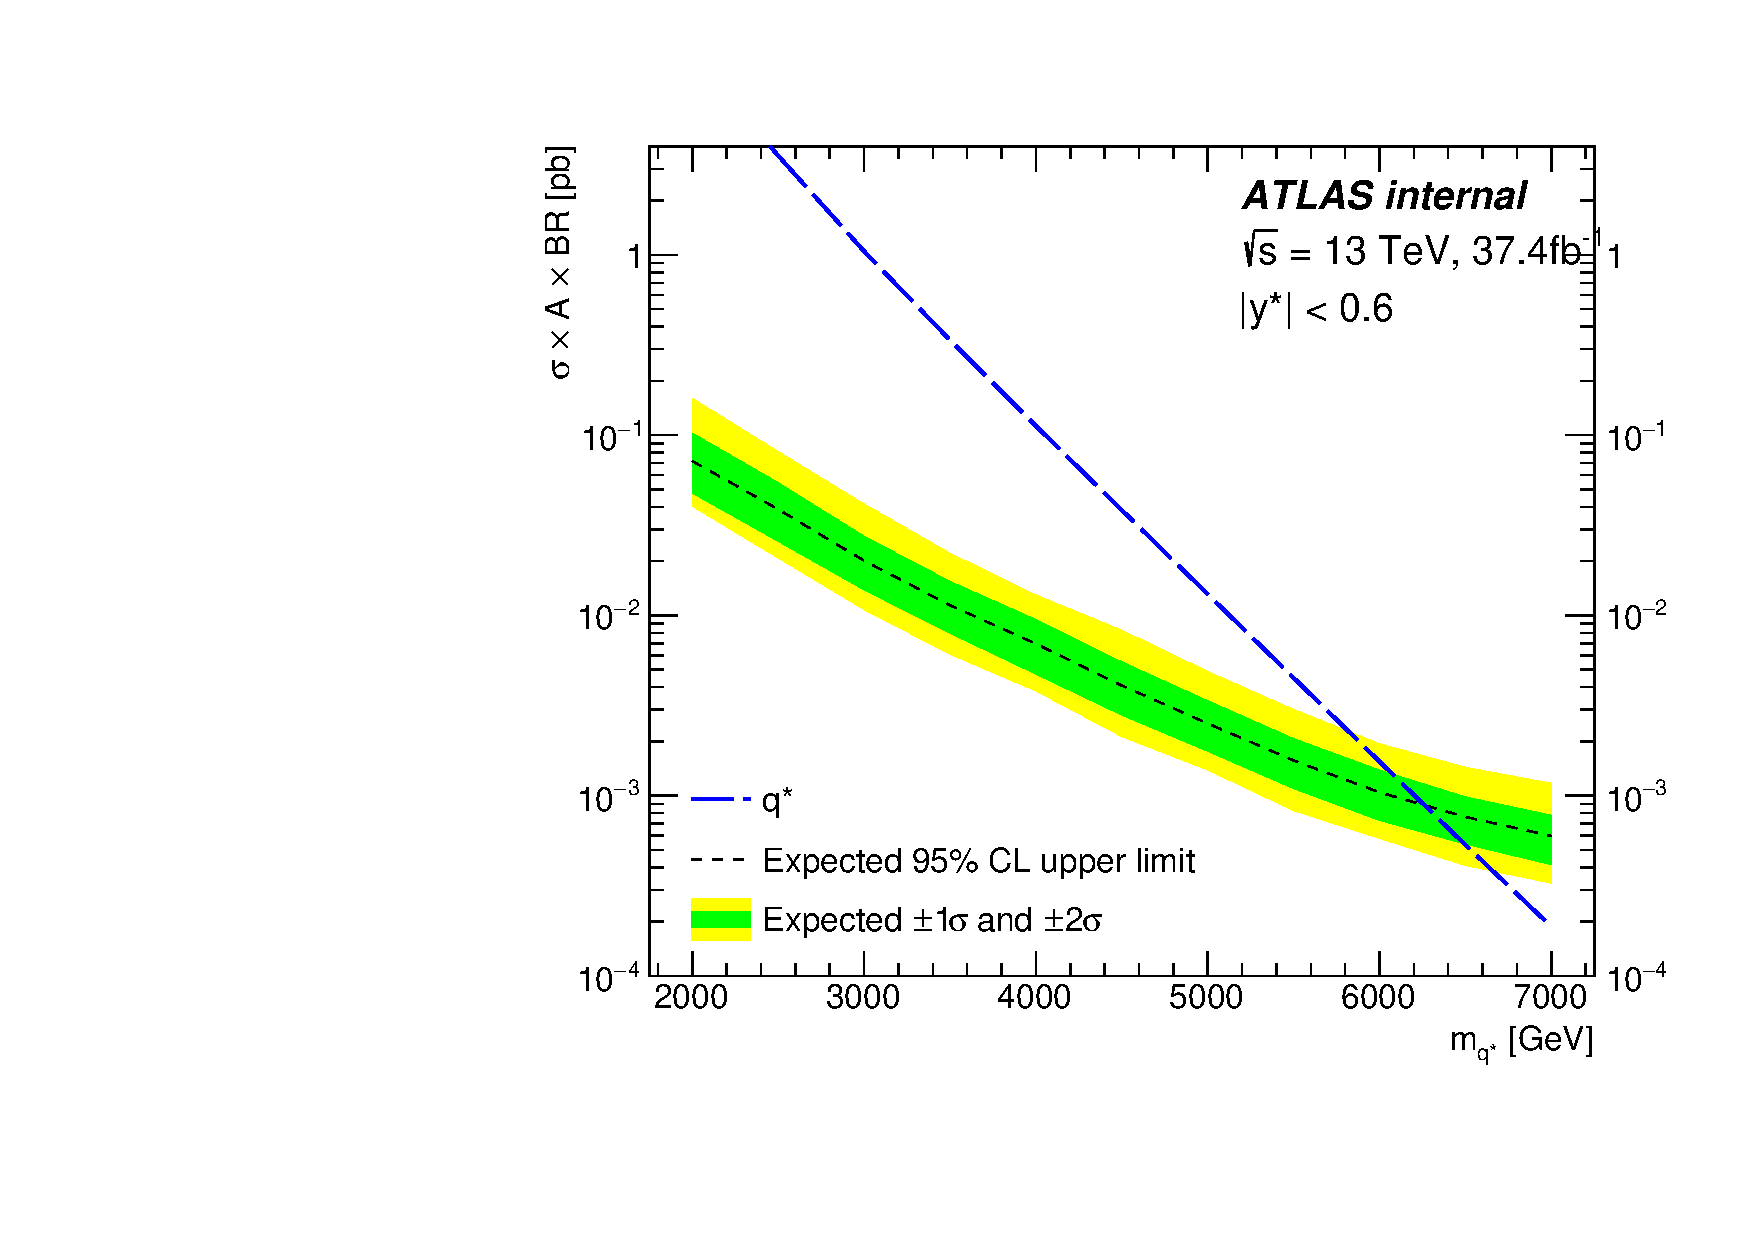
\includegraphics[width=0.475\textwidth] {figures/tagging/brazil-qStarMorphSingleCombinedUpdated.pdf}}
% \vspace*{-2mm}\\
% %
% \subfigure[\QQ] {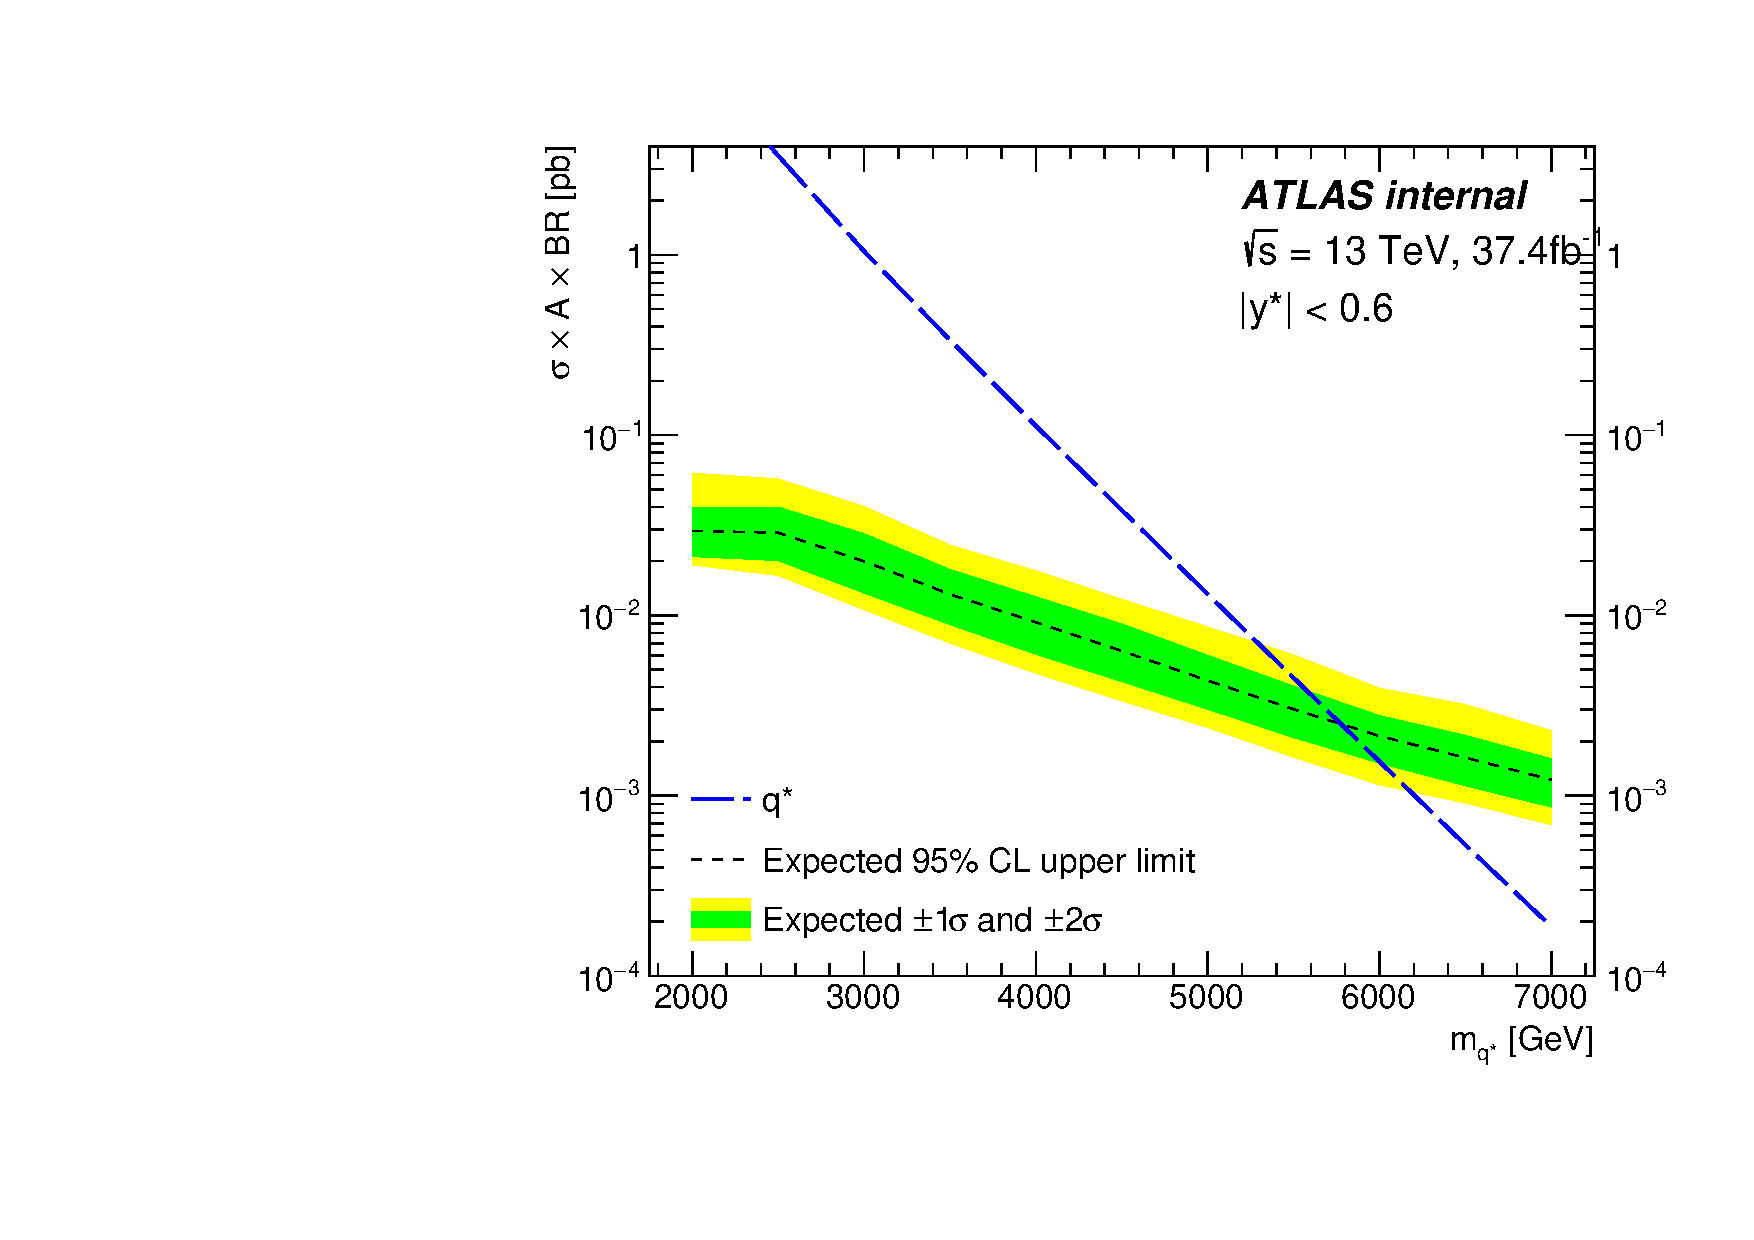
\includegraphics[width=0.475\textwidth] {figures/tagging/brazil-qStarMorphSingleQQUpdated}}
% \subfigure[\QG] {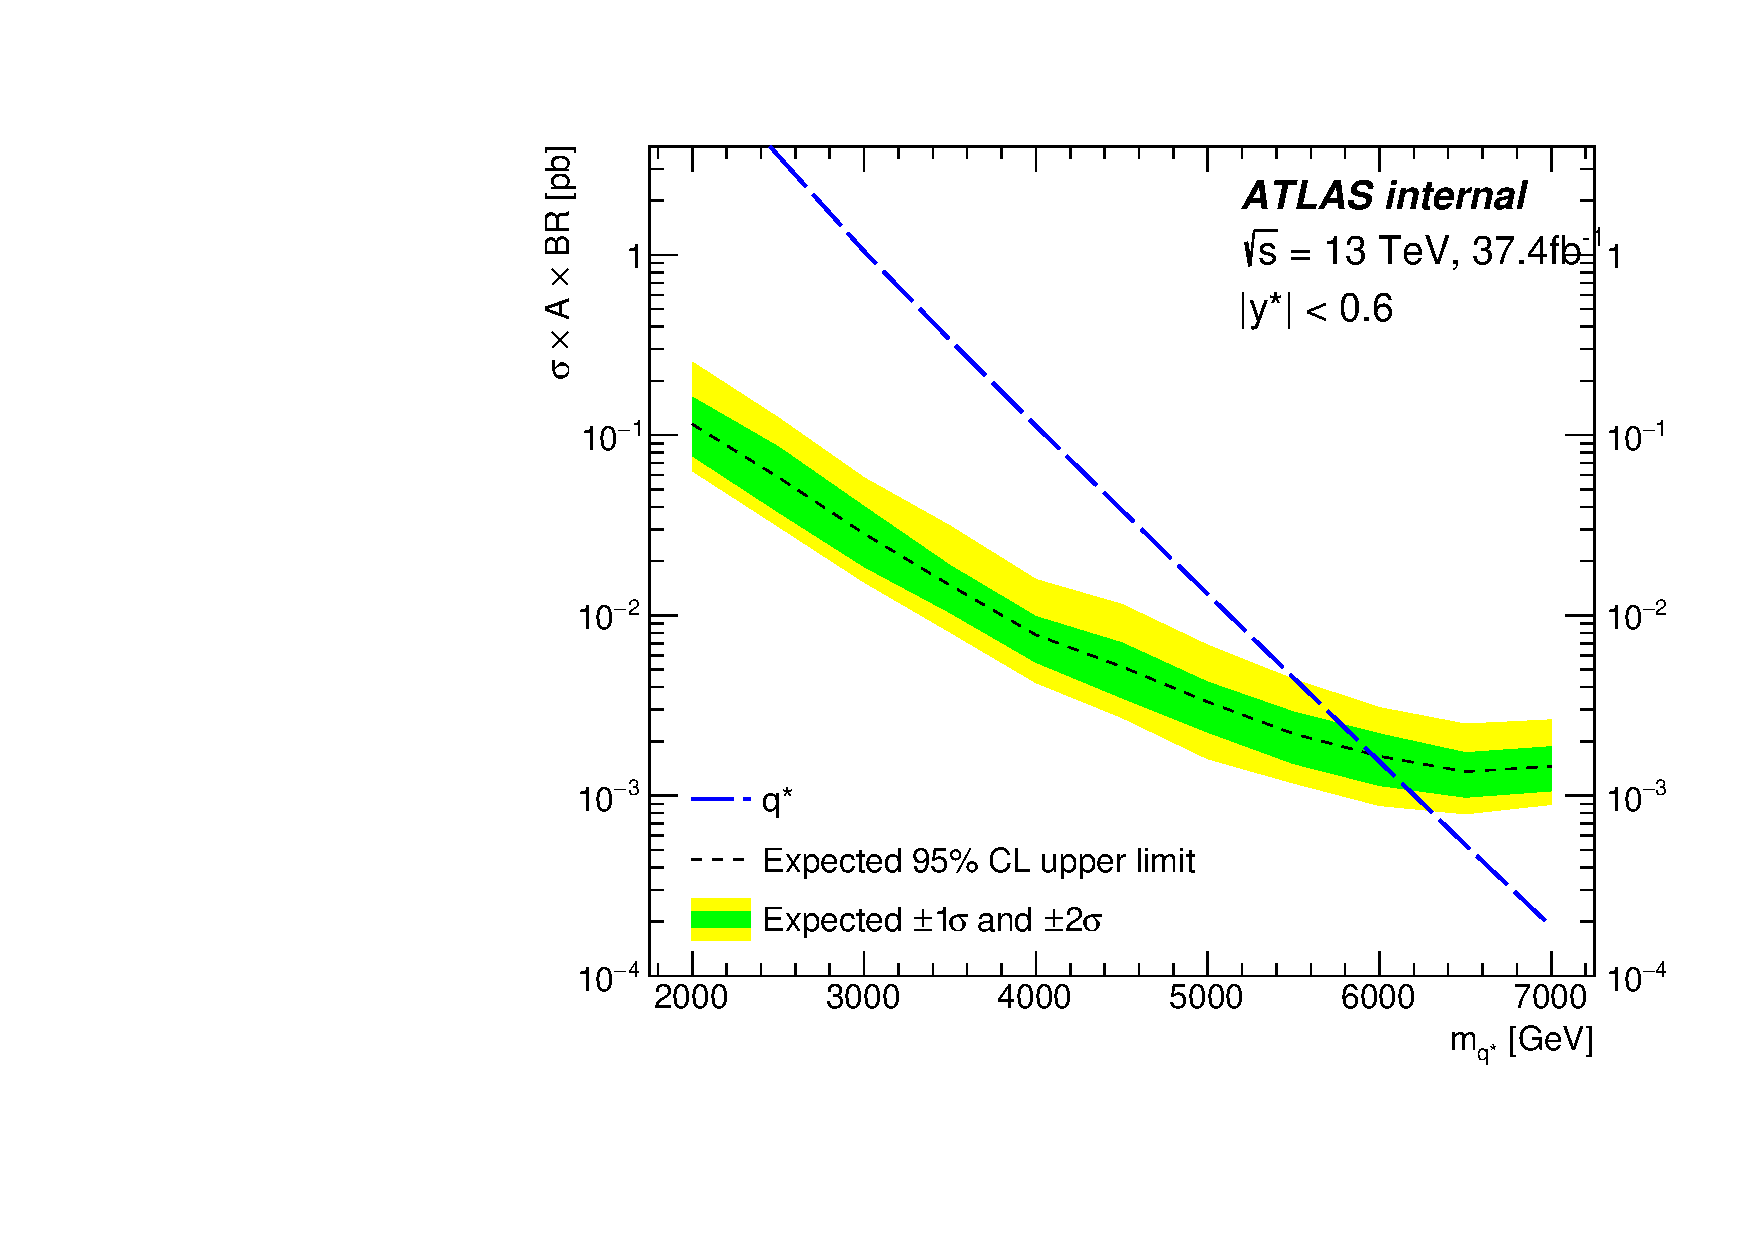
\includegraphics[width=0.475\textwidth] {figures/tagging/brazil-qStarMorphSingleQGUpdated}}
% \vspace*{-2mm}\\
% %
% \subfigure[\GG] {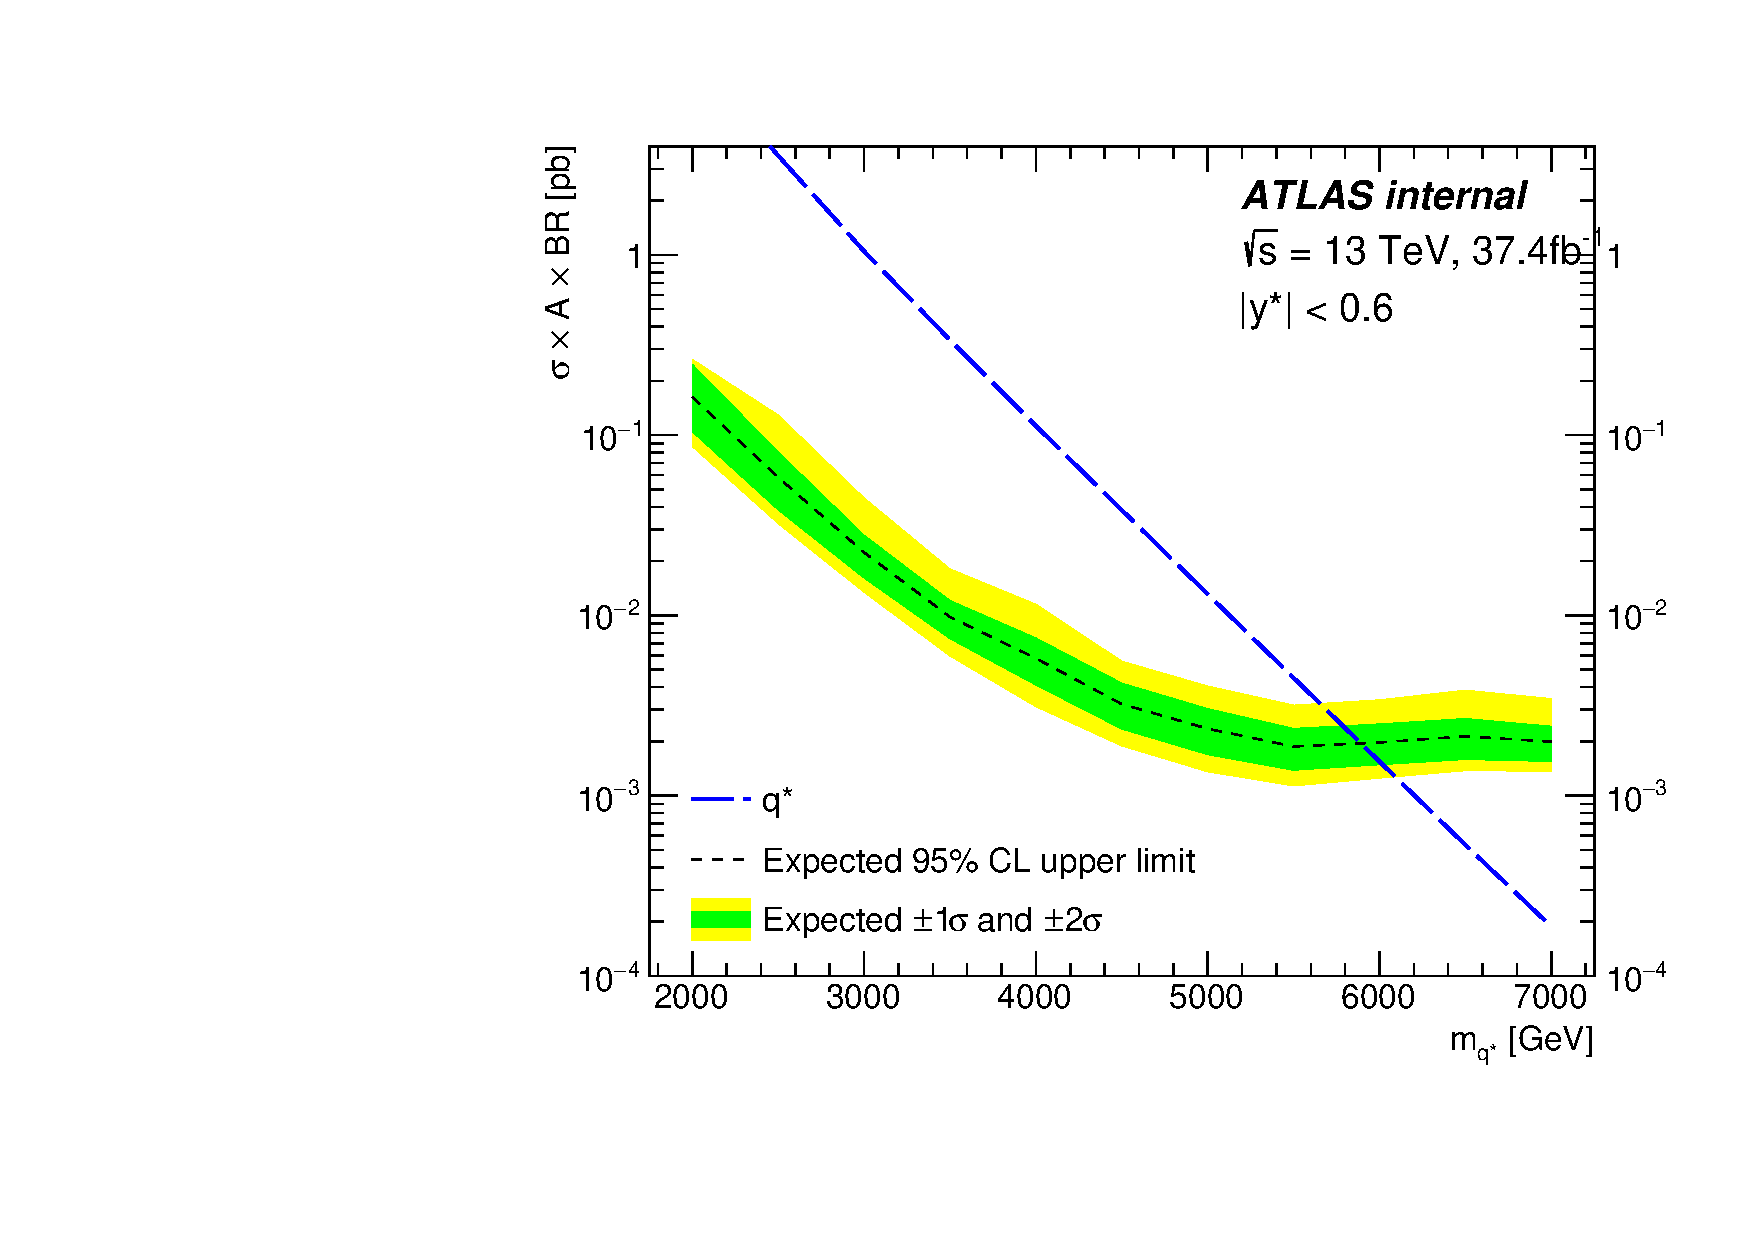
\includegraphics[width=0.475\textwidth] {figures/tagging/brazil-qStarMorphSingleGGUpdated}}
% \vspace*{-2mm}\\
% %
%
% \caption{Expected limits for a \qstar\ signal from  pseudo experiments for \integLumi\ for the 
% (a) \JJ\ resonant selection, (b) combined \QQ, \QG\ and \GG\ combined fit (c) \QQ\ sub-sample, (d) \QG\ sub-sample 
% and (e)  \GG\ sub-sample.
% \label{fig:toyMCExpectedLimitsqstar}}
%\end{figure}
%





\clearpage
%-------------------------------------------------------------------------------

%-------------------------------------------------------------------------------
\section{Event selection}
\label{sec:event_selection}
A common, baseline selection is applied for the resonant  analyses of
the Run~2 data that is taken directly from ~\cite{Nishu:2646455}, as
described in Section~\ref{sec:base_selection}. 

%Then, specific cuts applied
%for the resonant analysis, tailored to improve the sensitivity, are described in Sections~\ref{sec:res_selection}. 

\subsection{Observables and Kinematic Variables}
\label{sec:observables}
In the Standard Model (SM), the main and predominant source of dijet
events is two-to-two scattering in QCD processes. The search exploits
two key properties of the background to enhance its sensitivity to new
physics signals:

\begin{itemize}
	\item The background at high $m_{jj}$ is a smooth and continuously falling spectrum.
	\item The background at high mass strongly peaks in the forward
direction, due to Rutherford $t$- and $u$-channel poles in the cross sections
for many individual scattering diagrams \cite{Harris:2011bh}.
\end{itemize}

Many of the possible signals for the dijet search would appear as a
resonance peak in \mjj, the invariant mass of the dijet system formed
from the two highest-\pT\ jets. Resonant signals have $\cos{\theta}$
distributions which, in contrast to Rutherford scattering, are either
isotropic or follow some polynomial in $\cos{\theta}$\footnote{See
Ref.~\cite{Harris:2011bh} p15 for a summary.}, giving them a distinct
angular distribution from QCD processes. For this reason, the \mjj\
search selects events with small angle separation via an upper limit on
\begin{itemize}
	\item \ystar = $(y_1-y_2)/2$
\end{itemize}
to enhance sensitivity to higher energies and enable probing the scale
of new phenomena. Where $y_{1,2}$ is the rapidity of the leading and
sub-leading jet. The value of the \ystar\ cut is optimized to reject
$t$-channel QCD while admitting the other types of signals.

\subsection{Jet Reconstruction and Calibration}
Jets are reconstructed with the \akt algorithm \cite{Cacciari:2008gp}
with a distance parameter of 0.4, as implemented in the \textsc{FastJet}
package~\cite{Cacciari:2011ma}. For these studies, we use jets
reconstructed from topological clusters using the procedures described
in \cite{ATLAS-CONF-2015-002}. For jet cleaning, the standard
\textit{Loose} jet quality cuts are used as discussed in
\cite{ATLAS-CONF-2015-029}. An event-based jet cleaning is applied to
reject any event with a leading or sub-leading jet flagged as
\textit{Bad} for the \textit{Loose} criteria.  The jet criteria used is
summarized in Table~\ref{tab:jetCalibration}.

\begin{table}[ht]
	\label{tab:jetCalibration}
		\begin{tabular}{|c|c|}
			\hline
			%\large
			\multicolumn{2}{|c|}{Jet reconstruction parameters} \\
			%\normalsize
			%\normalsize
			\hline
			Parameter & Value \\
			\hline
			Algorithm & \akt  \\
			R-parameter & 0.4 \\
			Input Constituent & EMTopo \\
			Analysis Release Number & 21.2.65 \\
			%Calibration tag & JetCalibTools-00-04-76 \\
			CalibArea tag & 00-04-82 \\
			Calibration configuration & JES\_data2017\_2016\_2015\_Consolidated\_EMTopo\_2018\_rel21.config \\
			Calibration sequence (Data) & JetArea\_Residual\_EtaJES\_GSC\_Insitu \\
			Calibration sequence (MC) & JetArea\_Residual\_EtaJES\_GSC\_Smear \\
			Calibration configuration (AFII) & JES\_MC16Recommendation\_AFII\_EMTopo\_April2018\_rel21.config \\
			Calibration sequence (AFII) & JetArea\_Residual\_EtaJES\_GSC \\
			\hline
			%\large
			\multicolumn{2}{|c|}{Selection requirements} \\
			%\normalsize
			\hline
			Observable & Requirement \\
			\hline
			Jet cleaning & Loose WP \\
			Batman cleaning & No \\
			\pT  & $>$150 GeV \\
			\textbar$\eta$\textbar & $<$5.0 \\
			\hline
	\end{tabular}
\caption{Jet selection criteria used in this analysis.}
\end{table}


\subsection{Trigger}
The data used in this analysis are collected using the lowest
unprescaled small-R single-jet trigger.  The naming convention of
single-jet triggers follows either `Jnnn' for L1 triggers or `jnnn' for
HLT trigger, where 'nnn' is a number specifying the nominal jet \pT
threshold for the trigger in \GeV\.  The energy scale of the trigger
threshold is the EM scale for L1 triggers, while a calibration sequence
very close to what is applied to offline jets is applied to HLT jets,
bringing their scale to the hadronic scale.\\

The lowest single jet un-prescaled trigger in 2015 was HLT\_j360, in
2016 was HLT\_j380, in 2017 was HLT\_j420 (if we ignore one run with
luminosity around 2\,\ipb ) and in 2018 was also HLT\_j420. So to keep
the selection consistent across years, the kinetic requirement derived
for HLT\_j420 is used for the analysis. In addition to this,
HLT\_j225\_gsc420\_boffperf\_split is also unprescaled for all data
taking and also considered for the trigger studies for the analysis. \\

For the complete \RunTwo dataset, the two single-jet unprescaled
triggers for all data taking are: HLT\_j420 and
HLT\_j225\_gsc420\_boffperf\_split as mentioned above, both of which are
seeded from the L1\_J100 trigger. Both triggers search for jets with
$\pT > 420 \GeV$, while the HLT\_j225\_gsc420\_boffperf\_split trigger
also applies the offline global sequential calibration (GSC) to improve
the trigger turn-on.\\

The trigger turn-on was investigated in Ref.~\cite{Nishu:2646455}
finding that  obtaining the turn-on directly from \mjj\ provides a much
lower turn-on than from requiring a specific cut on the leading jet \pT.
As such, the analysis does not require an explicit cut on the \pT\ of
either the leading or subleading jet. In practice, the invariant mass
cut imposes a soft cut of 420~\GeV on the leading jet, and 150~\GeV on
the subleading jet. The two triggers are very similar in performance,
and having one over another does not change our lower \mjj\ threshold
from the binning.


In order not to sculpt the \mjj\ distribution in an odd way due to
different triggers and given the assessment of the turn-on, the analysis
uses the HLT\_j420 trigger with no cut on the leading jet \pT.

\subsection{Baseline selection}
\label{sec:base_selection}
The baseline event selection is applied for all signal regions and
the cuts applied are:
\begin{itemize}
\item Good Run List (GRL): Requirement that all relevant detectors were in a good state ready for physics. The GRLs used for this analysis are:
	\begin{itemize}
		\item 2015(3.2\,\ifb): data15\_13TeV.periodAllYear\_DetStatus-v89-pro21-02\_Unknown\_PHYS\_ \newline StandardGRL\_All\_Good\,\_25ns.xml
		\item 2016(32.97\,\ifb): data16\_13TeV.periodAllYear\_DetStatus-v89-pro21-01\_DQDefects-00-02-04\_ \newline PHYS\_StandardGRL\_All\_Good\_25ns.xml
		\item 2017(44.31\,\ifb): data17\_13TeV.periodAllYear\_DetStatus-v99-pro22-01\_Unknown\_ \newline PHYS\_StandardGRL\_All\_Good\_25ns\_Triggerno17e33prim.xml
		\item 2018(59.94\,\ifb): data18\_13TeV.periodAllYear\_DetStatus-v102-pro22-04\_Unknown\_PHYS\_ \newline StandardGRL\_All\_Good\_25ns\_Triggerno17e33prim.xml
	\end{itemize}
\item LAr: Liquid Argon Calorimeter error rejected ( errorState(xAOD::EventInfo::LAr) )
\item Tile: Tile Calorimeter error rejected ( errorState(xAOD::EventInfo::Tile) )
\item SCT: SCT single event upsets rejected ( errorState(xAOD::EventInfo::SCT) )
\item Core: Incomplete event build rejected ( isEventFlagBitSet(xAOD::EventInfo::Core, 18) )
\item All jets with $\pt\ge 150~\GeV$ pass LooseBad cleaning cuts
\item Primary Vertex: the highest $\sum\pt^{2}(trk)$ (xAOD::VxType::VertexType::PriVtx) vertex has at least two tracks associated with it
\item Trigger: Passes the lowest unprescaled single-jet trigger, HLT\_j420
\item Jet preselecton: Leading jet $\pt\ge 380~\GeV$ and Jet multiplicity $\ge 2$
\end{itemize}

Additional kinematic selection criteria are used for the resonance to optimise the search potential and ensure good tracking efficiency. 

The following cuts are applied to the H$^\prime$ search.
\begin{itemize}
\item $|\Delta\phi| > 1.0$
\item $|\ystar| < 0.6$
\item $\mjj > 1100~\GeV$
\end{itemize}

The following cuts are applied to the string resonace search.
\begin{itemize}
\item $|\ystar| < 0.8$
\item $\mjj > 1717~\GeV$
\end{itemize}

The above cuts define the inclusive samples.
The following additonal cuts are for quark-gluon tagging.
\begin{itemize}
\item $|\eta| < 0.21$ (both jets)
\item $\ge 1$ gluon tagged (75\% working point)
\item 2 gluons tagged (75\% working point)
\end{itemize}

\noindent
where the 75\% gluon selecton criteria is $n{500} > -7.26742 + 4.16218\ln(\pt)$.

\subsection{Basic kinematic plots}
\label{sec:kinematic_distributions}

%In this section a selection of kinematic and monitoring plots produced with the resonant selection on the full dataset is shown 
%(Figures~\ref{fig:monitoring1}, %\ref{fig:monitoring2}, \ref{fig:monitoring3}, 
%\ref{fig:monitoring5}, \ref{fig:monitoring6}). These plots are relative to \integLumi of data collected in 2015 and 2016.
% GRL has been applied here.
%
%\begin{figure}[htb]
% \centering
% \subfigure[] {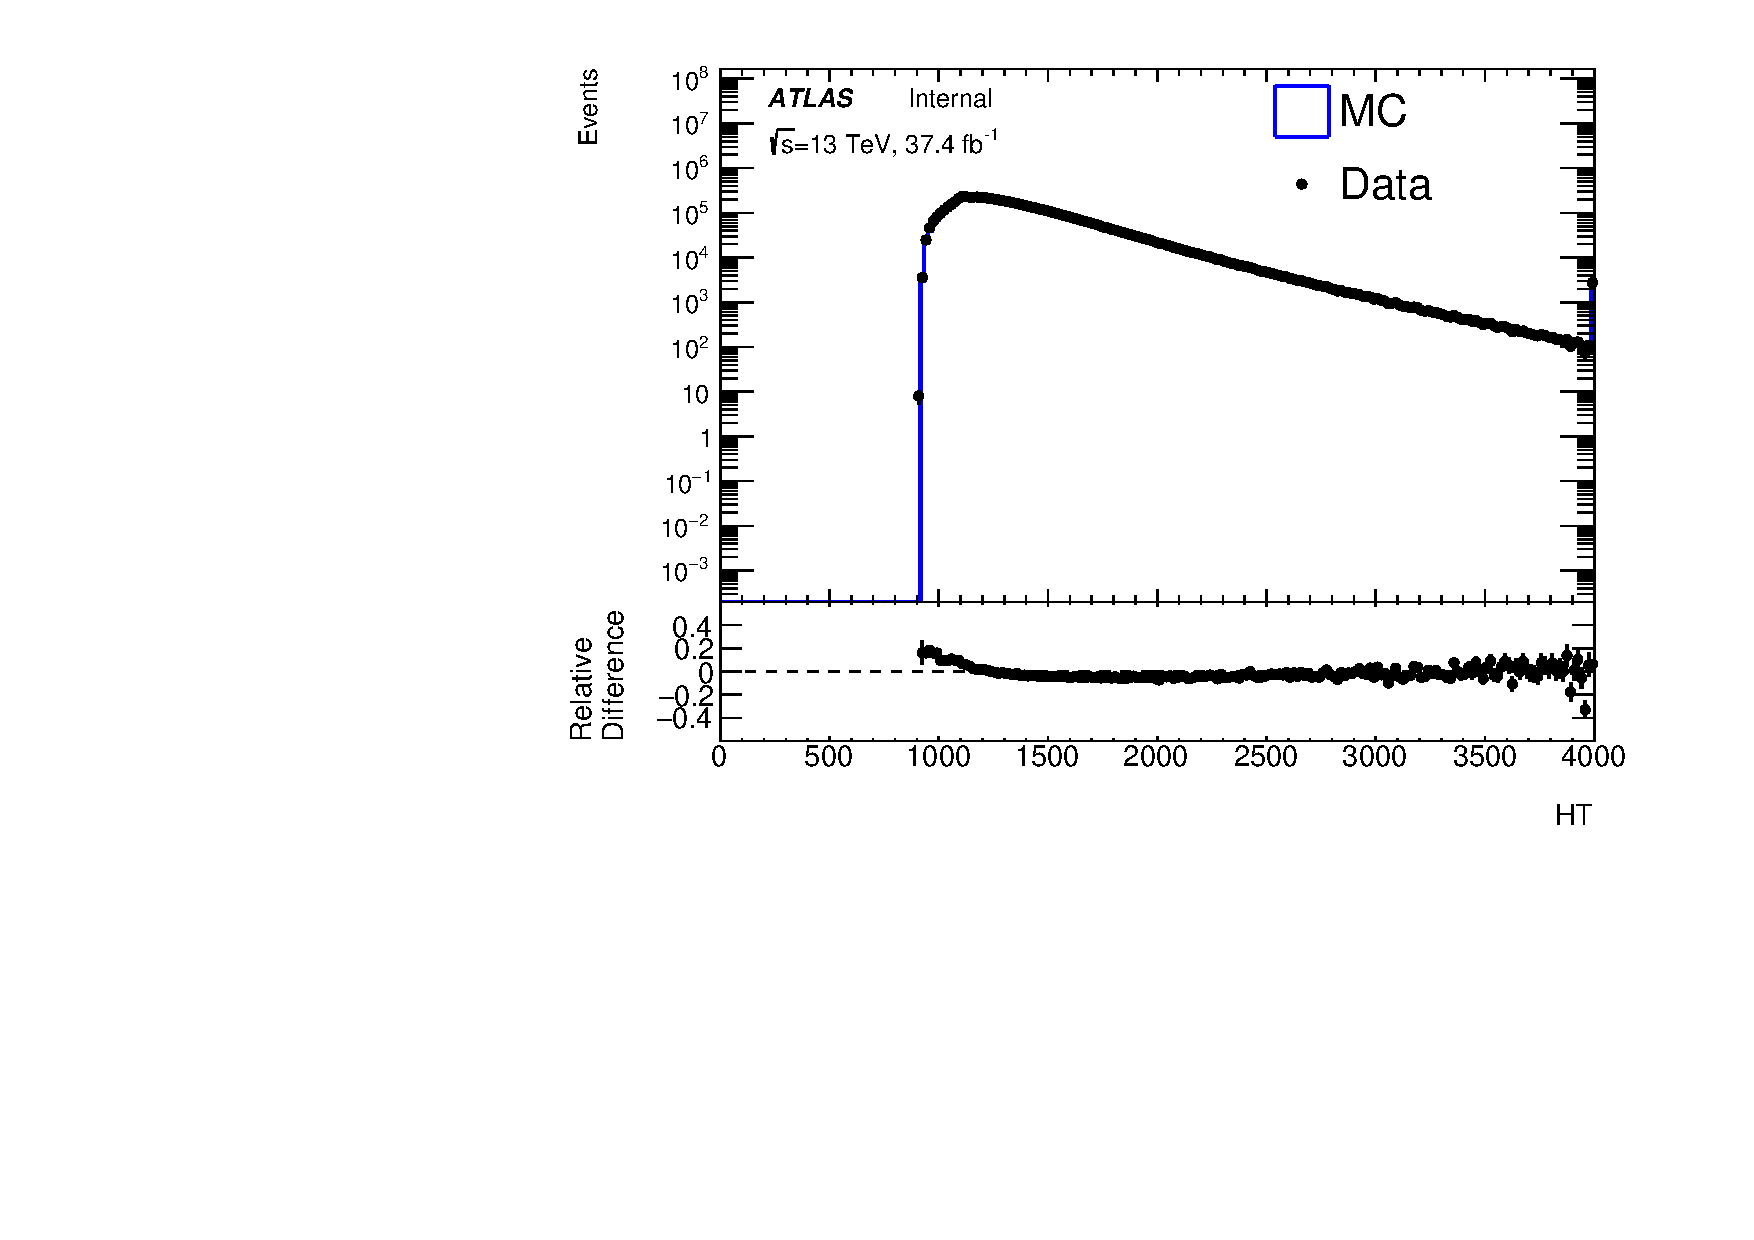
\includegraphics[width=0.45\textwidth]{figures/monitoring/resonant/Moriond_2017/newStudy_HT_logY.pdf}}
% \subfigure[] {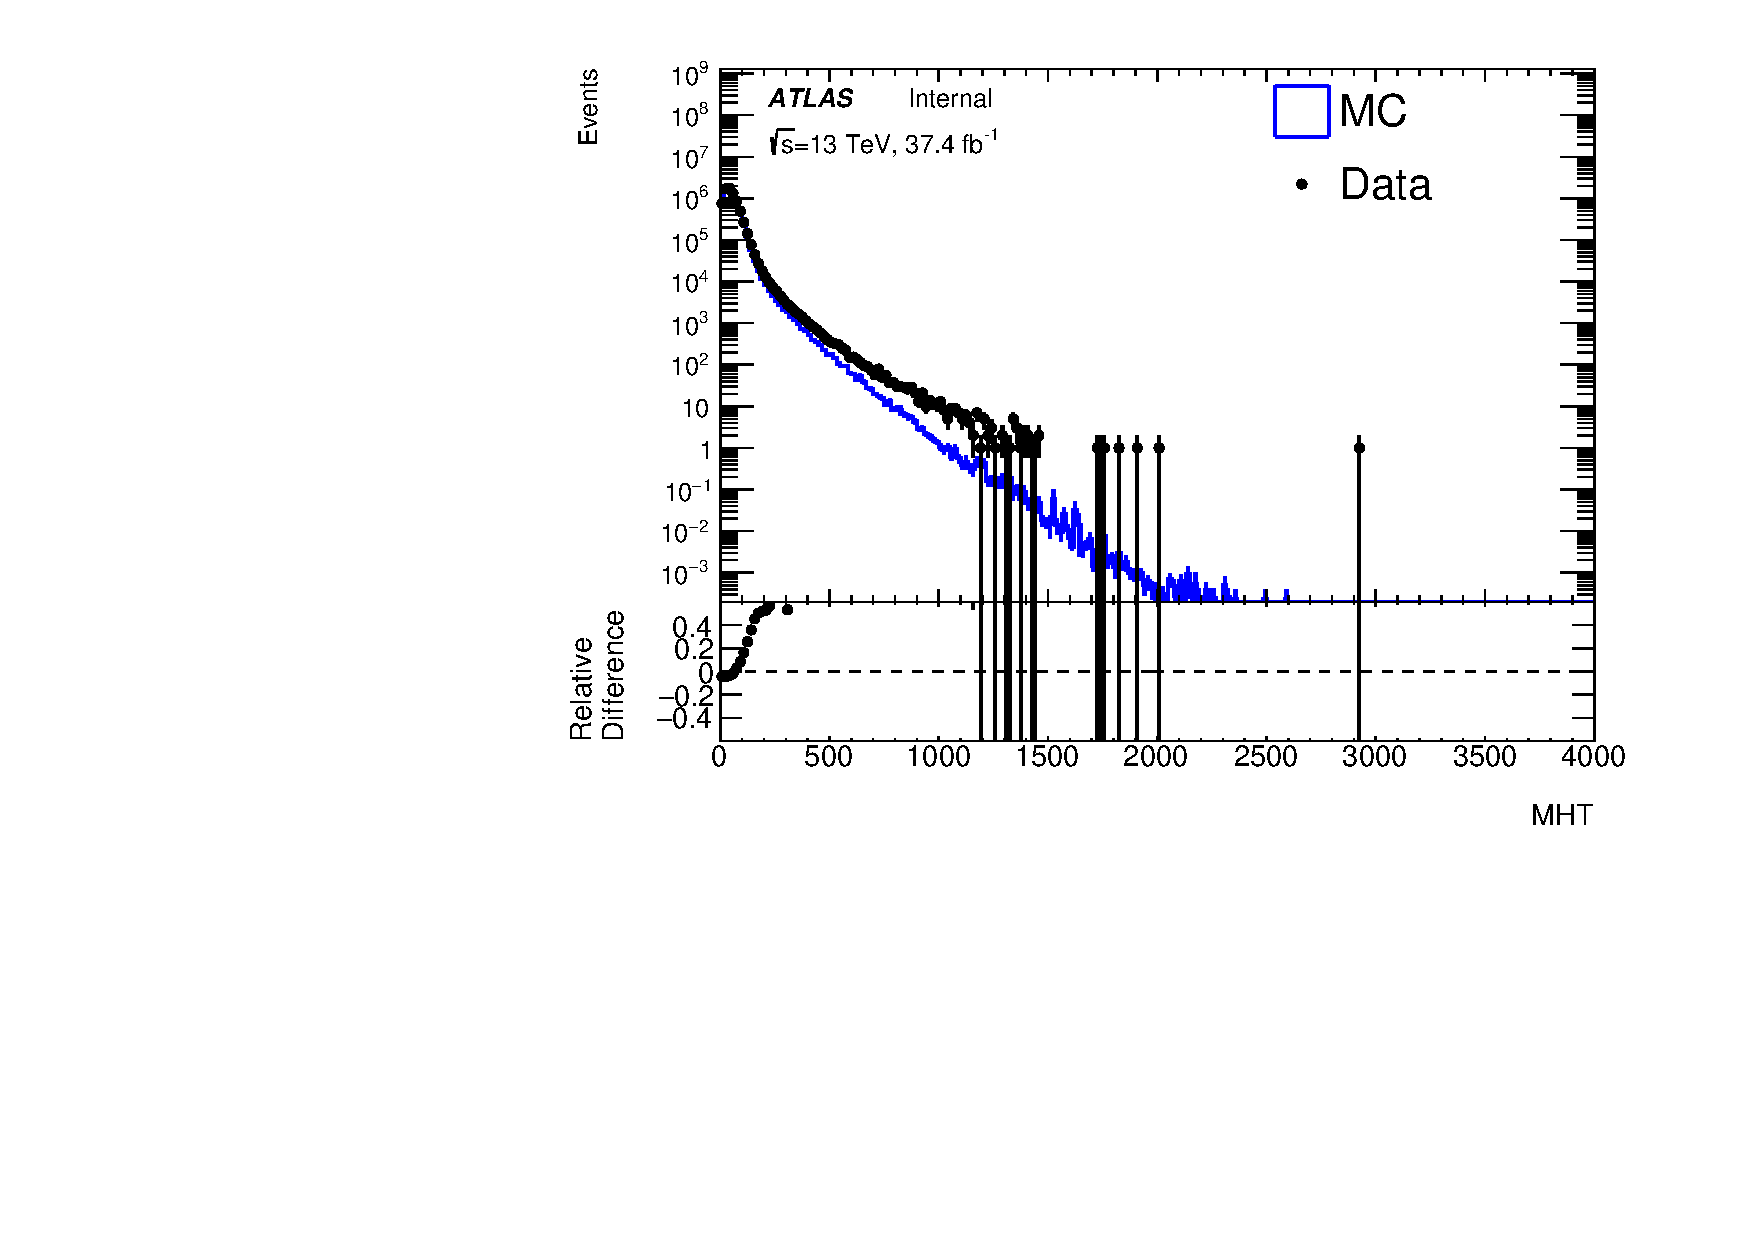
\includegraphics[width=0.45\textwidth]{figures/monitoring/resonant/Moriond_2017/newStudy_MHT_logY.pdf}}
% %
% \subfigure[] {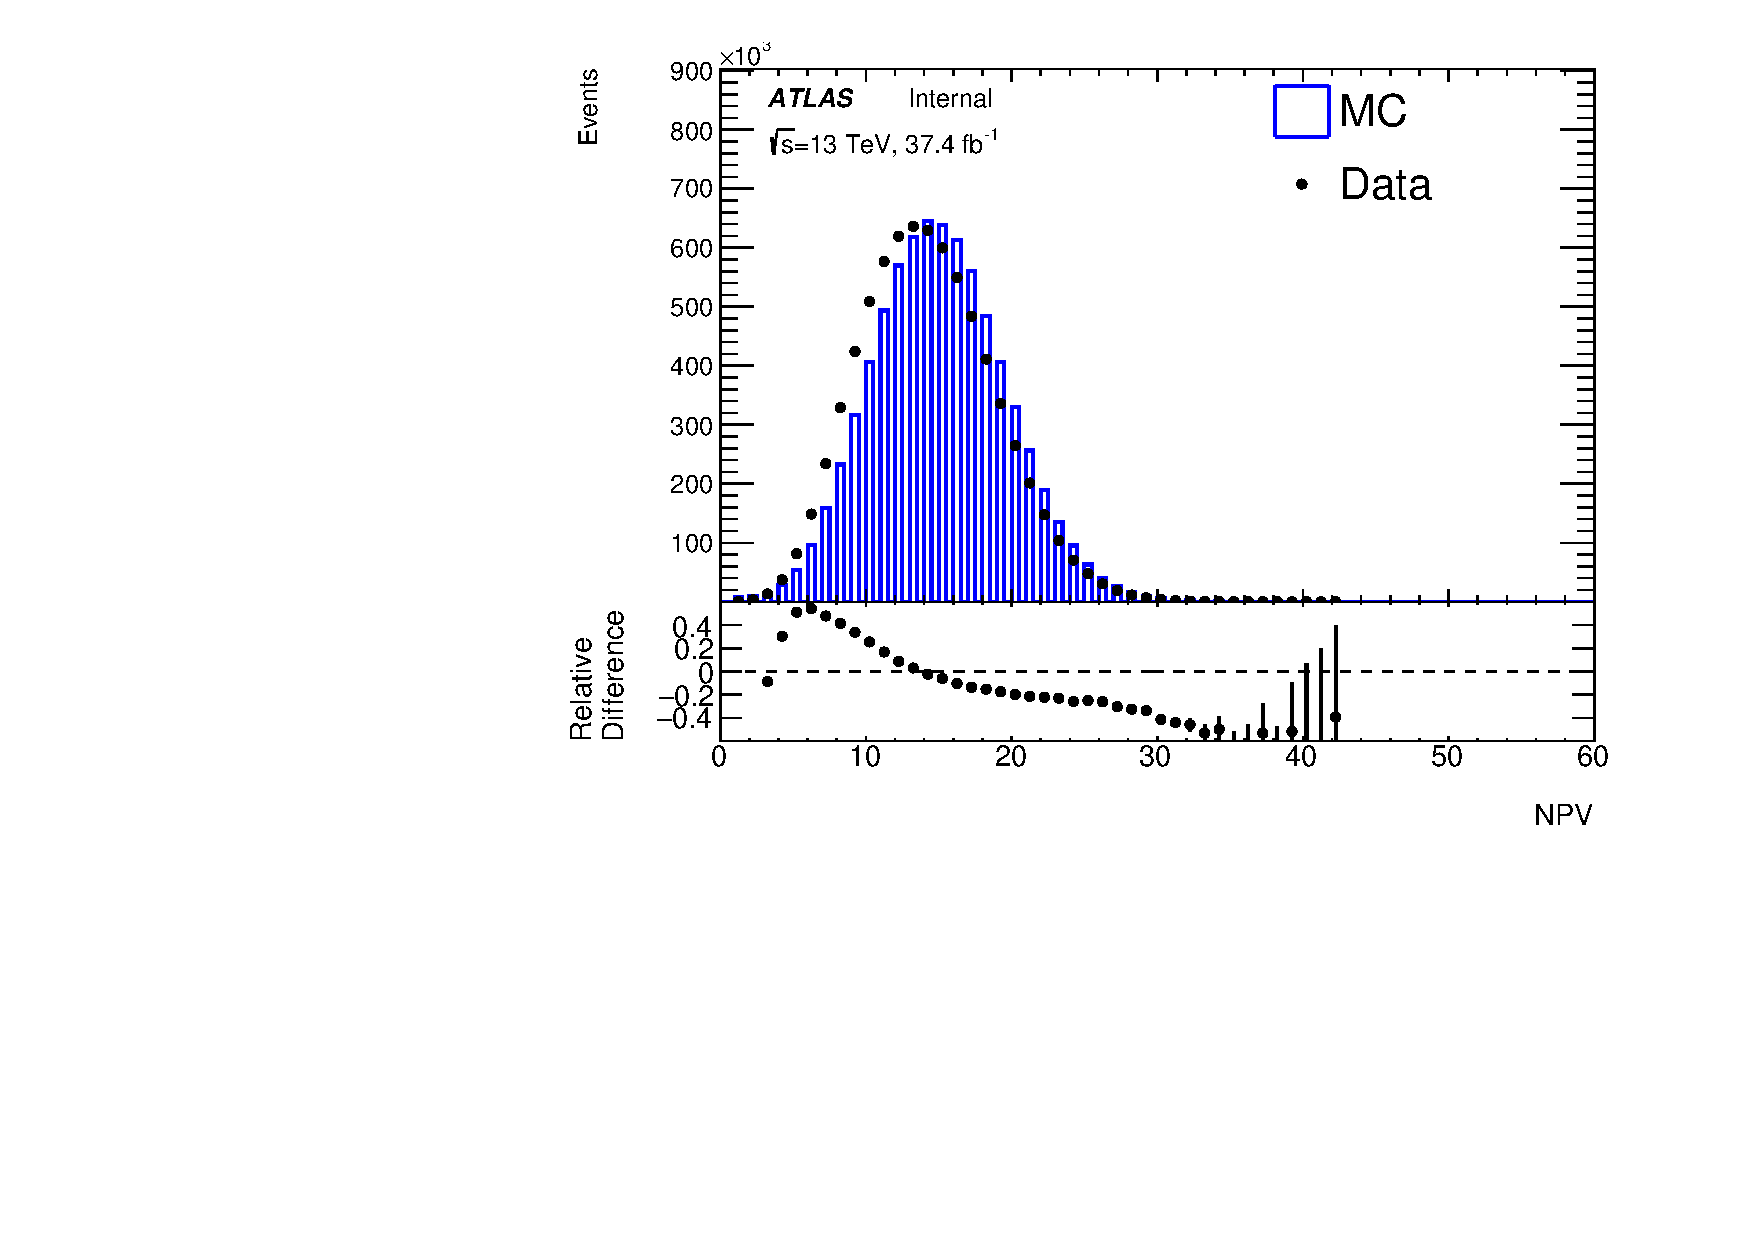
\includegraphics[width=0.45\textwidth]{figures/monitoring/resonant/Moriond_2017/newStudy_NPV.pdf}}
% \subfigure[] {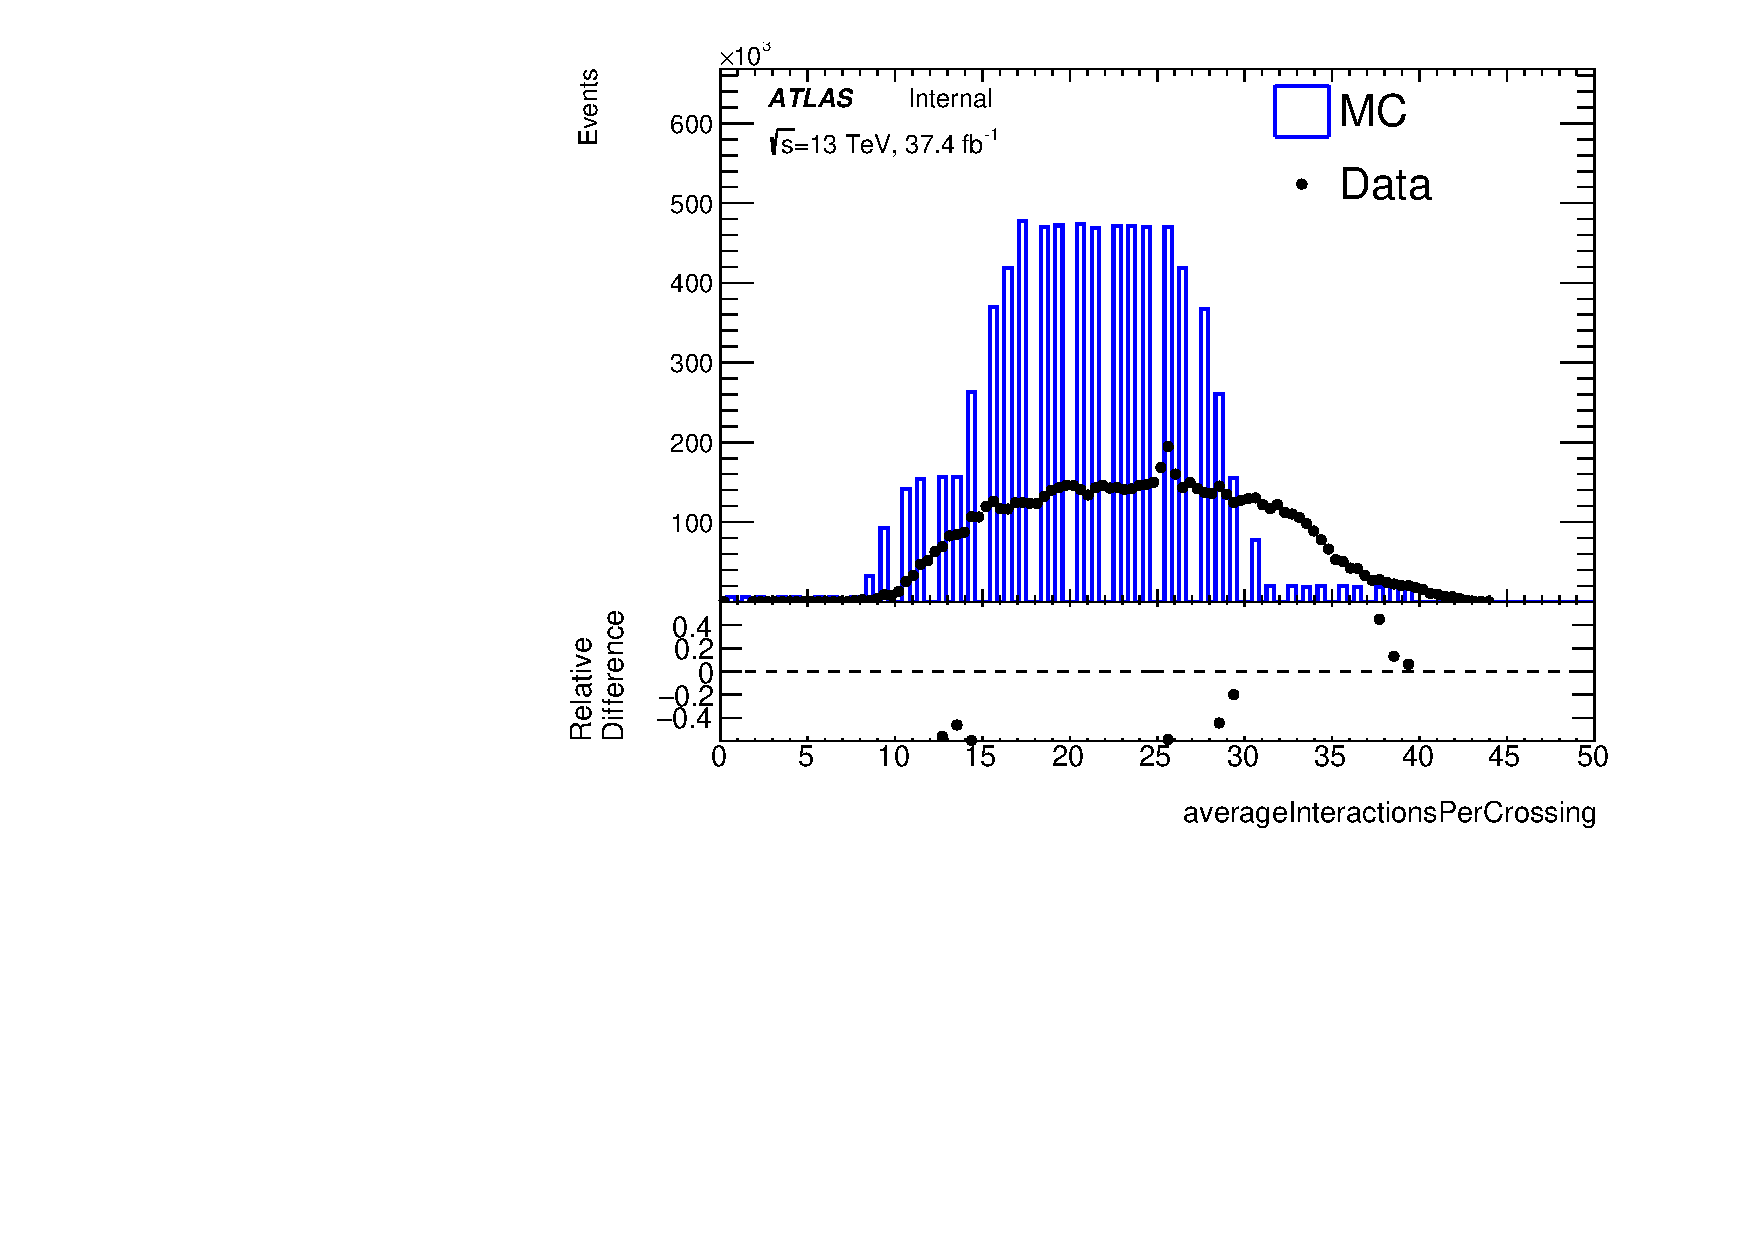
\includegraphics[width=0.45\textwidth]{figures/monitoring/resonant/Moriond_2017/newStudy_averageInteractionsPerCrossing.pdf}}
% \caption{Monitoring plots on %2016 data, 
% the resonant selection. (a) $H_T$, (b) $MH_T$ (missing transverse momentum calculated only from the jets in the event), (c) number of primary interaction vertices and (d) average interactions per bunch crossing.}
% \label{fig:monitoring1}
%\end{figure}
%
%
%\clearpage
%
%In this section a selection of kinematic and monitoring plots produced with the resonant selection on the complete resonance dataset is shown 
%(Figures~\ref{fig:JJmonitoring1},  
%\ref{fig:JJmonitoring5}, \ref{fig:JJmonitoring6}). These plots are relative to \integLumi of data collected in 2015 and 2016.
% GRL has been applied here.
%
%
%\begin{figure}[htb]
% \centering
% \subfigure[] {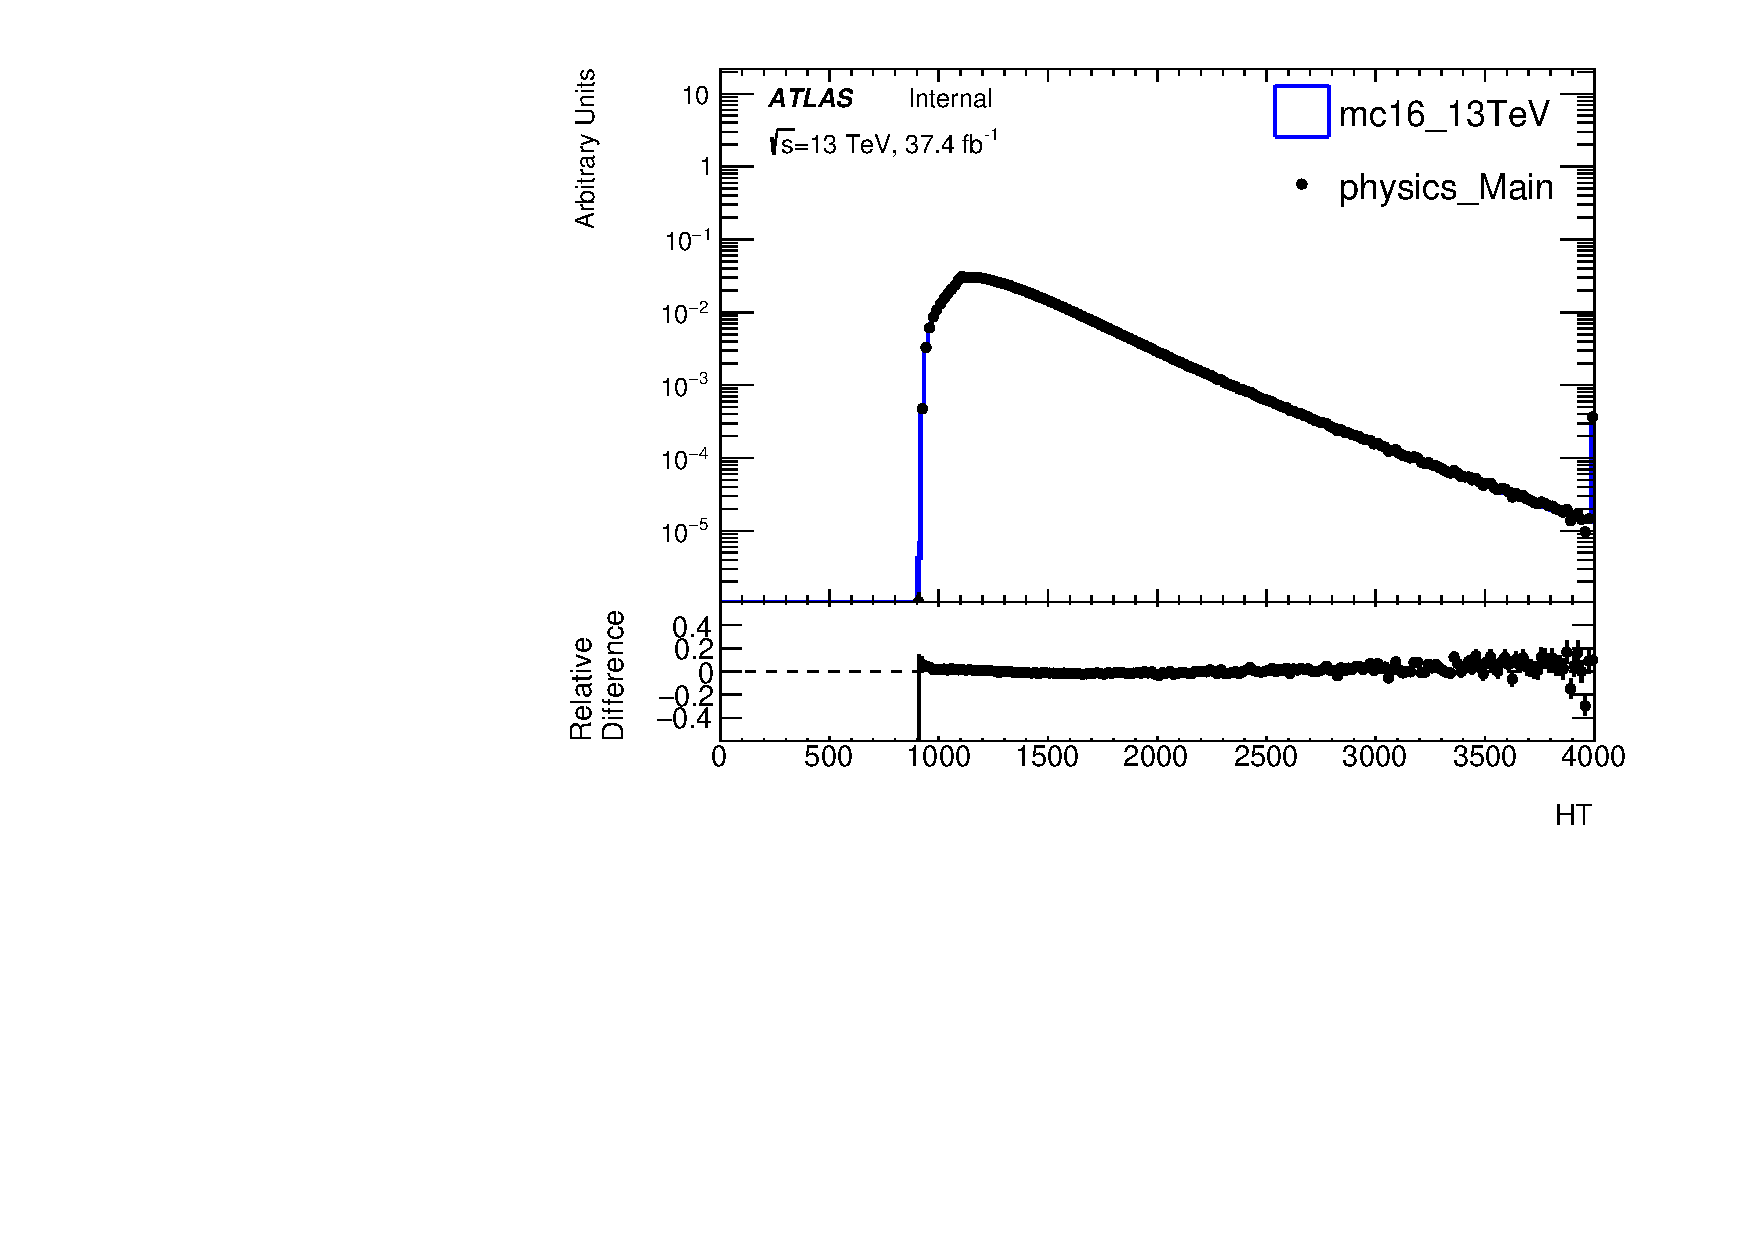
\includegraphics[width=0.45\textwidth]{figures/monitoring/resonant/2015-16/JJ/newStudy_HT_logY_JJv01.pdf}}
% \subfigure[] {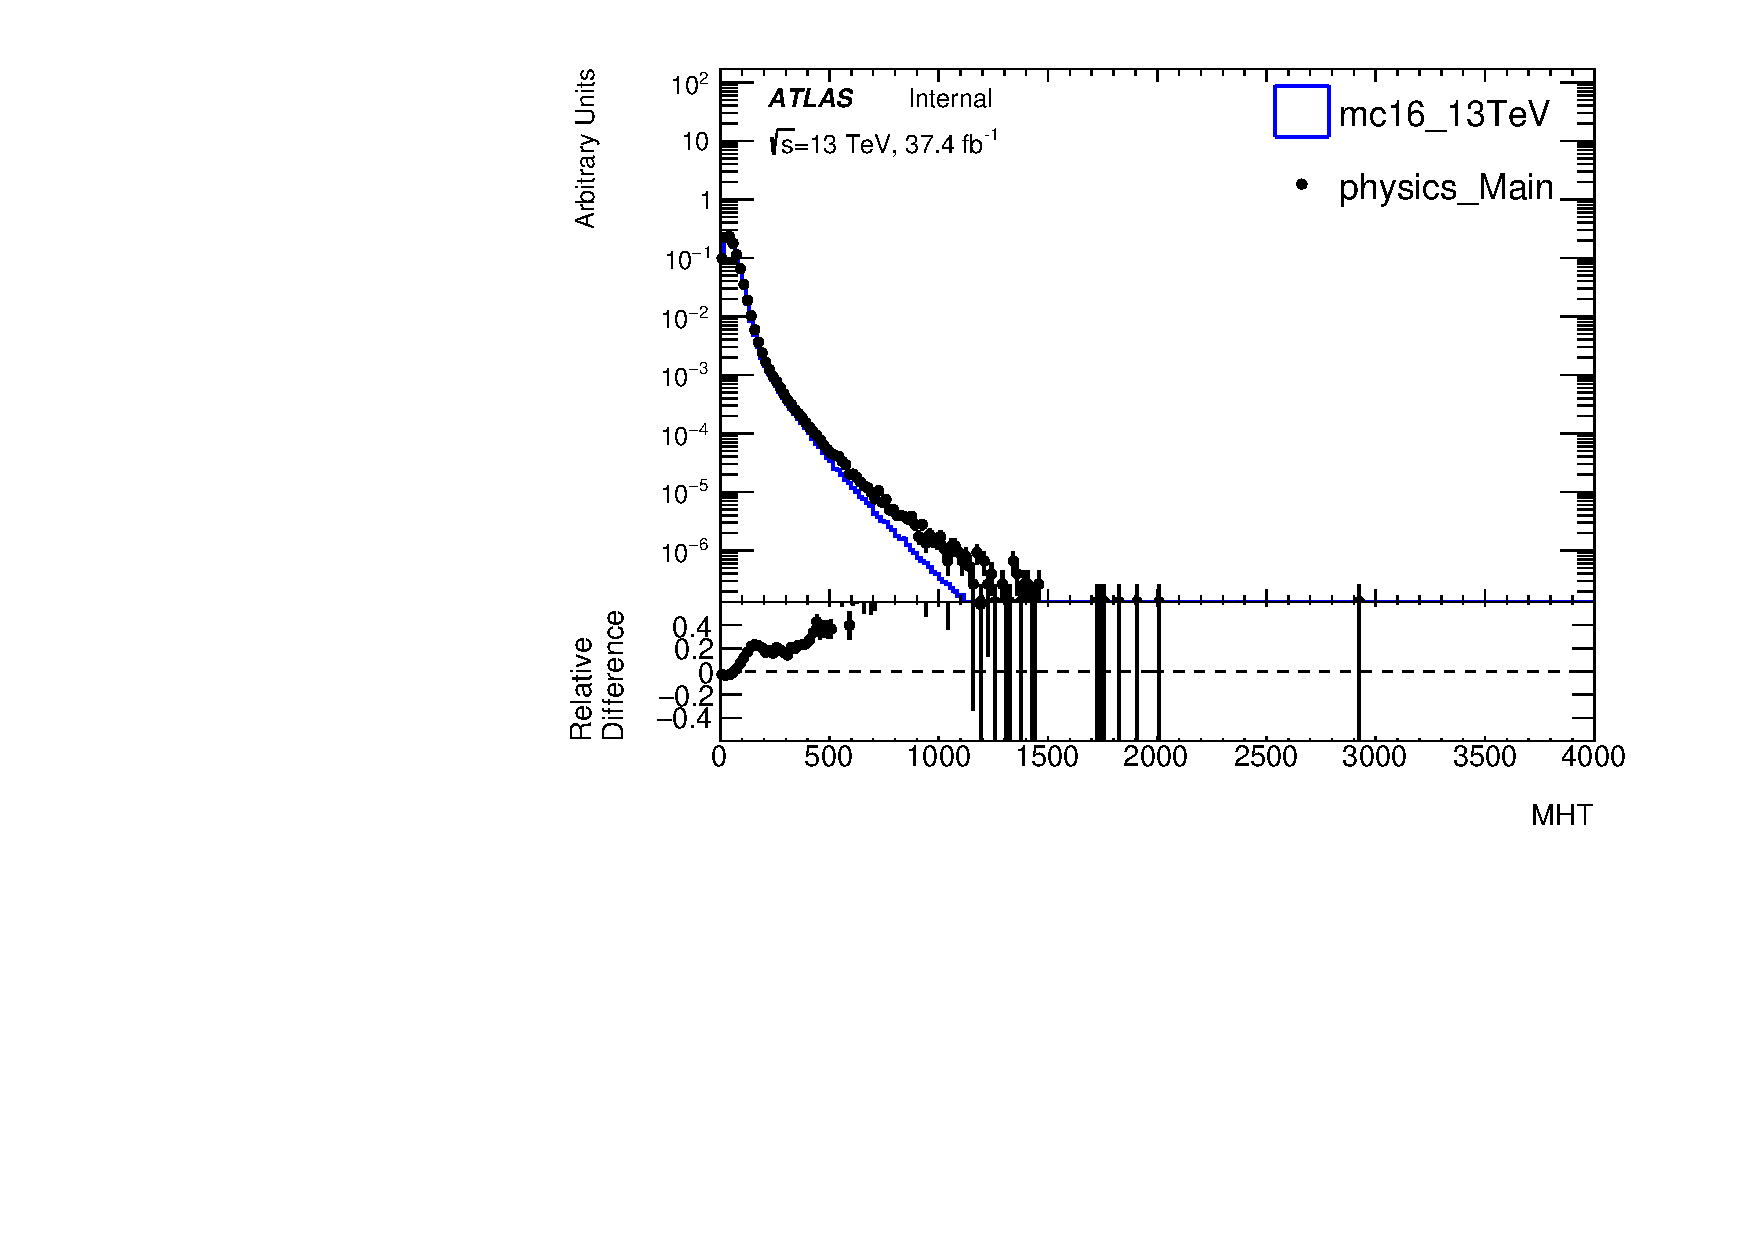
\includegraphics[width=0.45\textwidth]{figures/monitoring/resonant/2015-16/JJ/newStudy_MHT_logY_JJv01.pdf}}
% %
% \subfigure[] {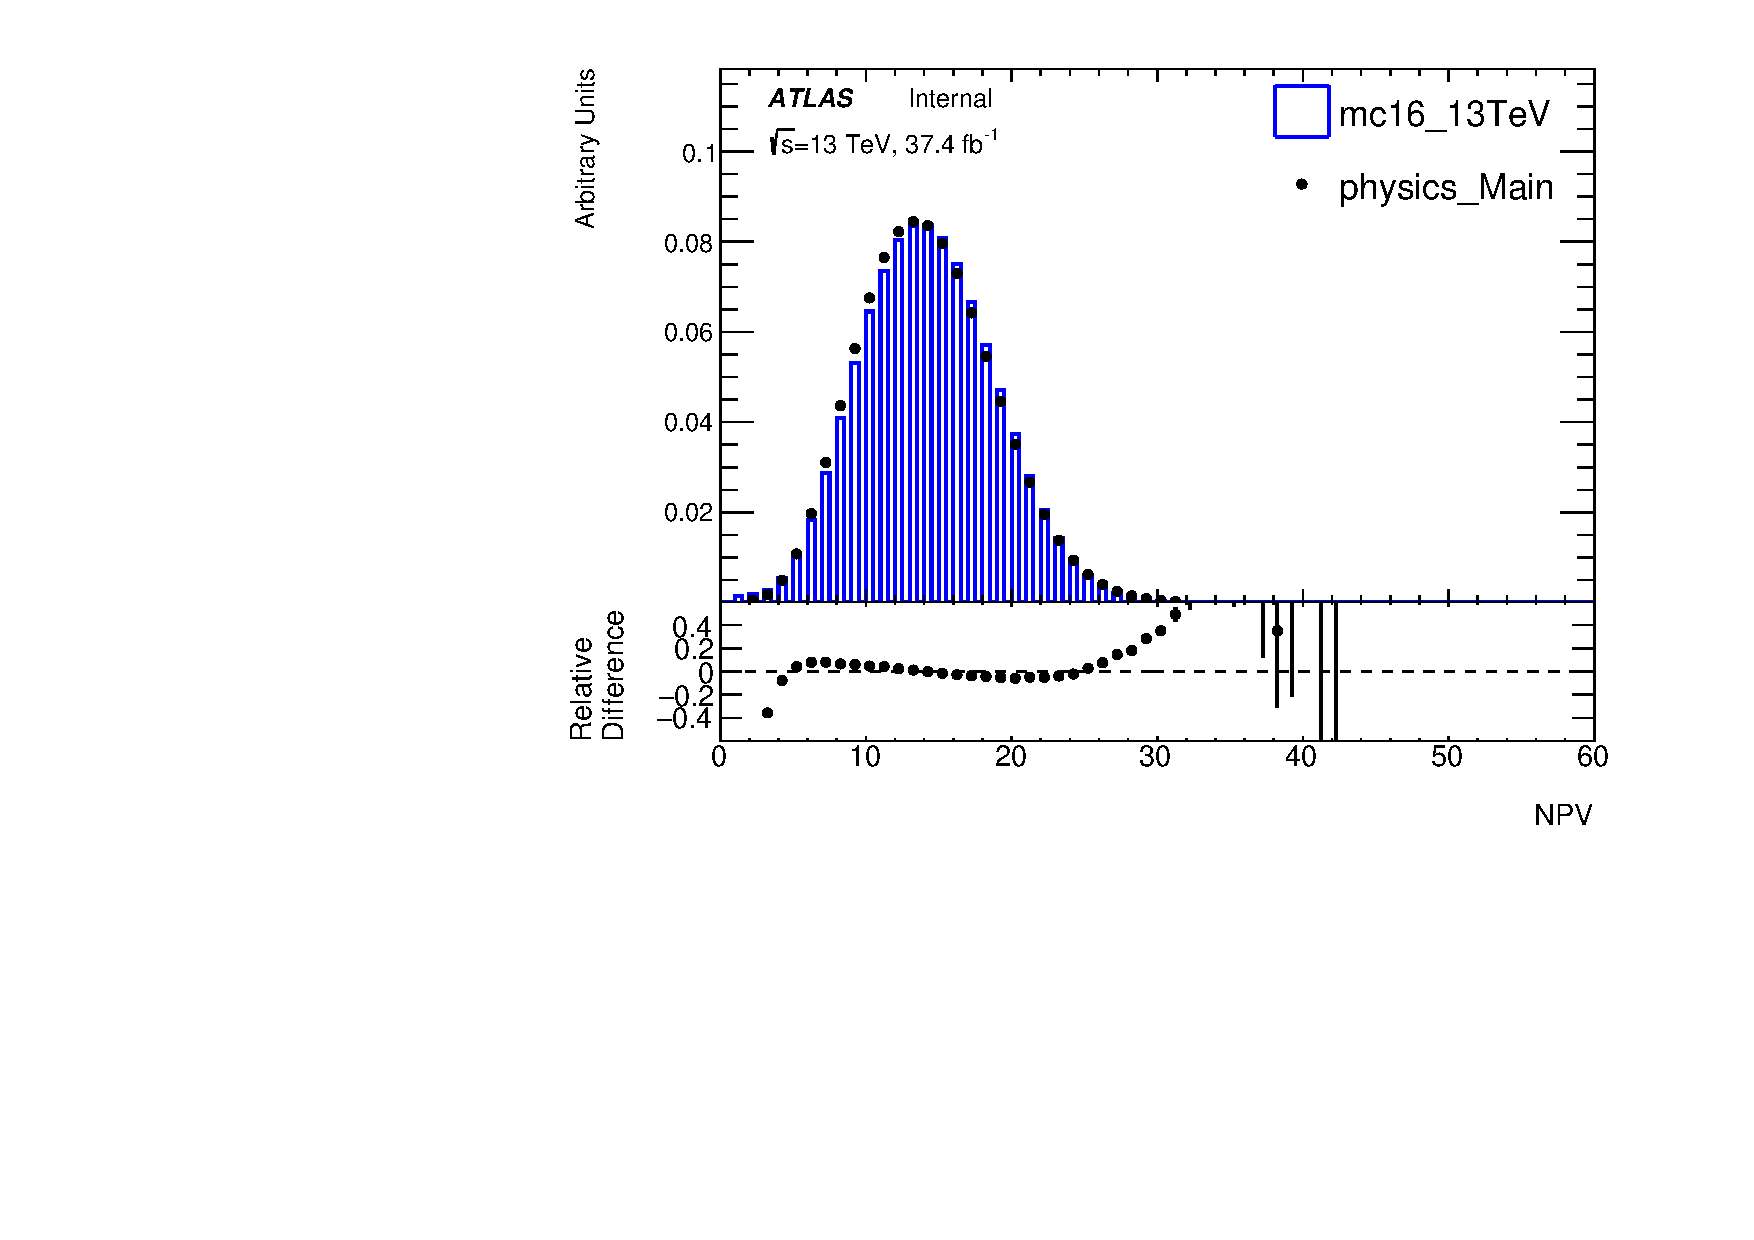
\includegraphics[width=0.45\textwidth]{figures/monitoring/resonant/2015-16/JJ/newStudy_NPV_JJv01.pdf}}
% \subfigure[] {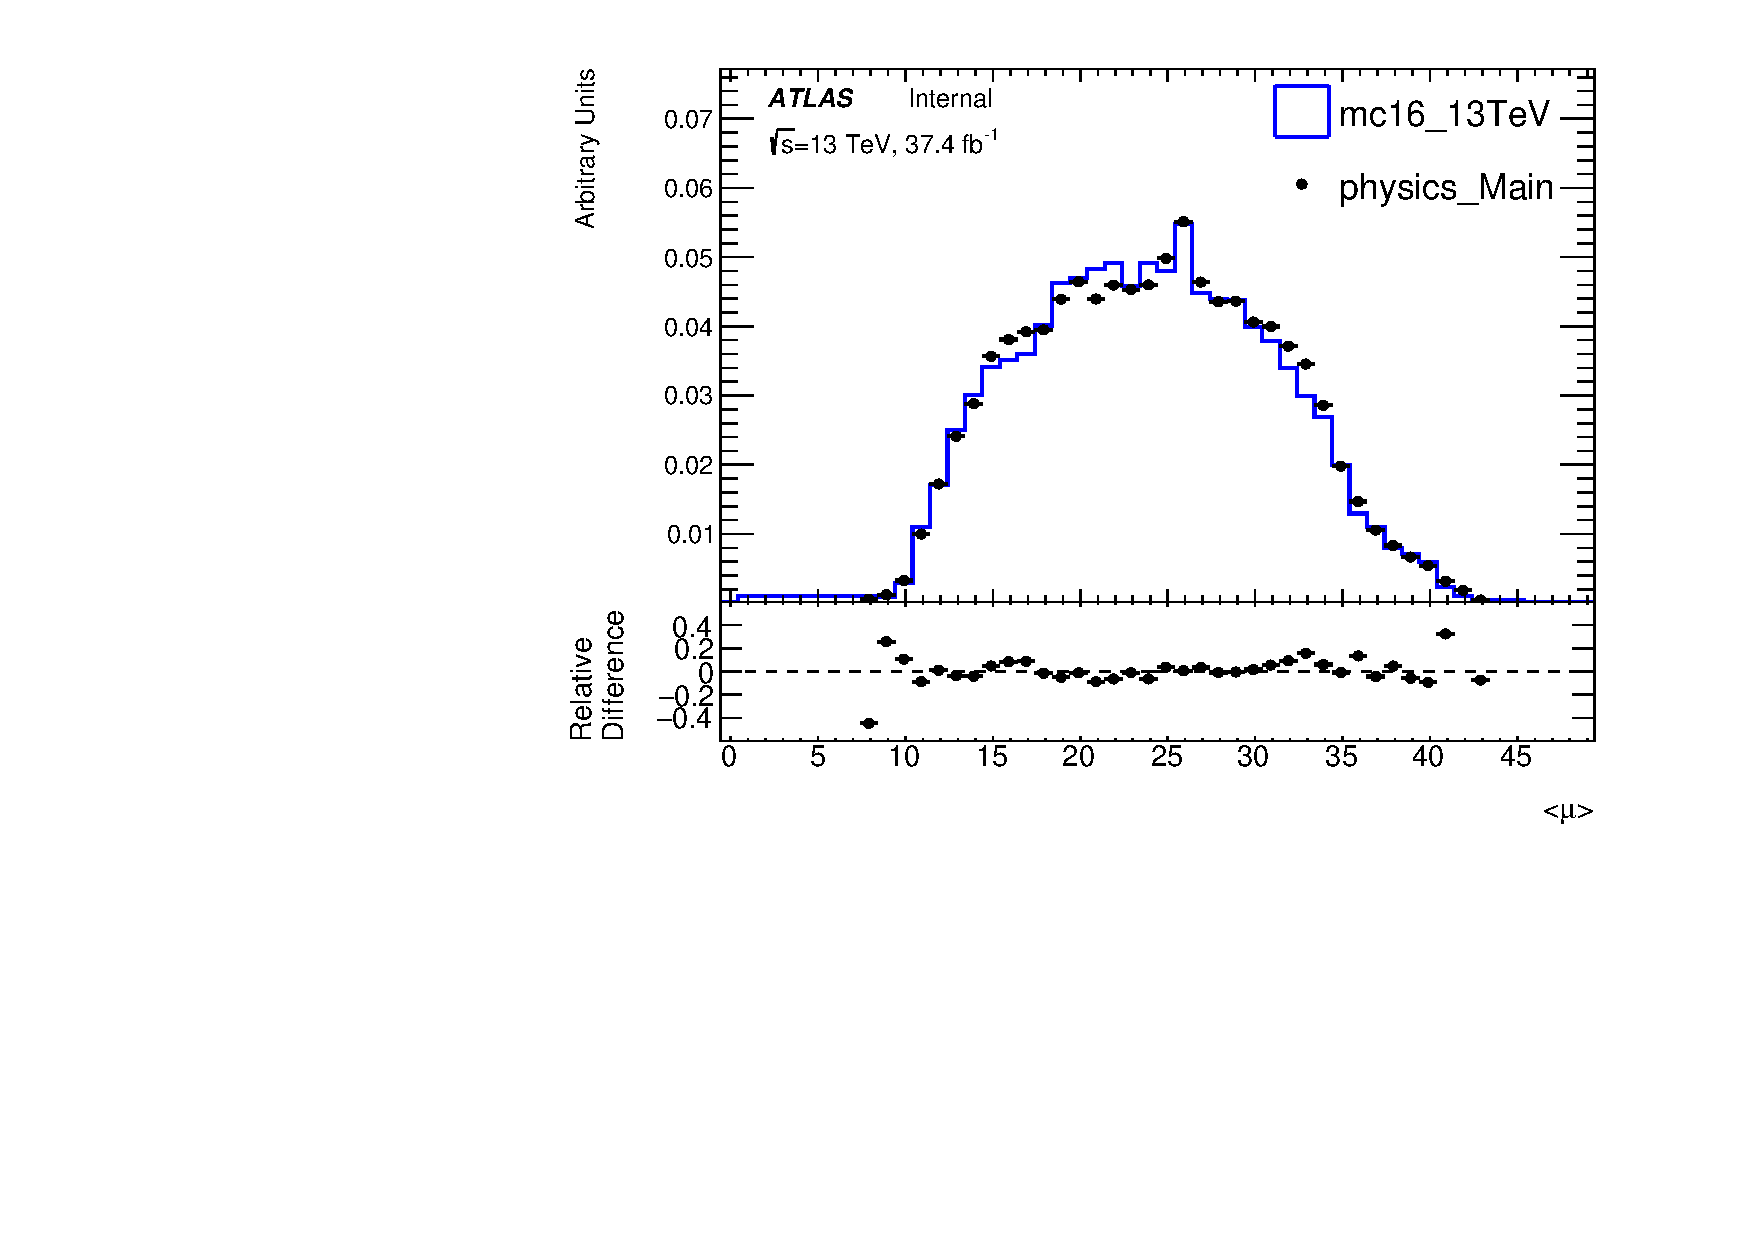
\includegraphics[width=0.45\textwidth]{figures/monitoring/resonant/2015-16/JJ/newStudy_averageInteractionsPerCrossing_JJv01.pdf}}
% %
%
% \caption{Monitoring plots on %2016 data, 
% the JJ resonant selection. (a) $H_T$, (b) $MH_T$ (missing transverse momentum calculated only from the jets in the event), (c) number of primary interaction vertices and (d) average interactions per bunch crossing.}
% \label{fig:JJmonitoring1}
%\end{figure}
%
% \begin{figure}[htb]
% \centering
%  %
% \subfigure[] {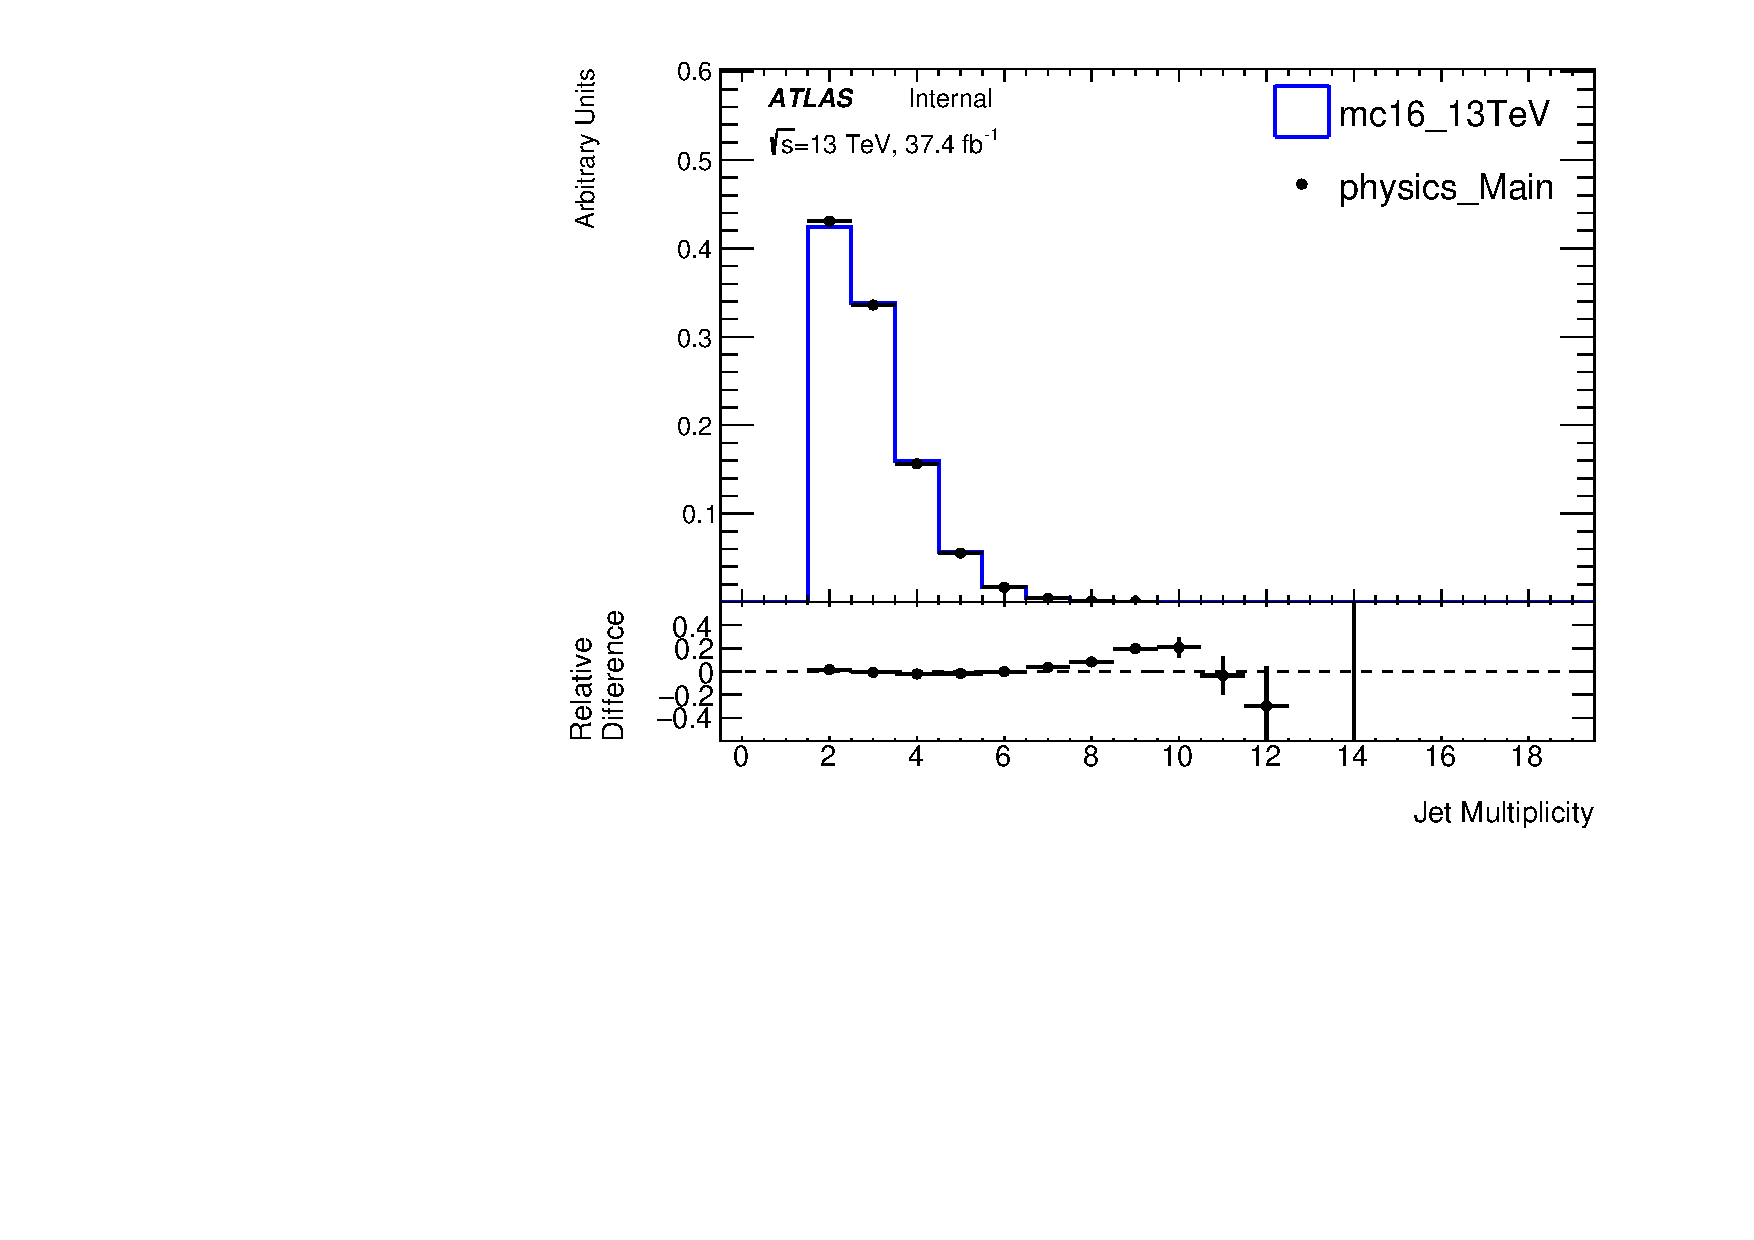
\includegraphics[width=0.45\textwidth]{figures/monitoring/resonant/2015-16/JJ/newStudy_njets_JJv01.pdf}}
% \subfigure[] {\includegraphics[width=0.45\textwidth]{figures/monitoring/resonant/2015-16/JJ//newStudy_deltaPhi_logY_JJv01.pdf}}
%
%%
% \subfigure[] {\includegraphics[width=0.45\textwidth]{figures/monitoring/resonant/2015-16/JJ/newStudy_jet_eta_logY_JJv01.pdf}}
% \subfigure[] {\includegraphics[width=0.45\textwidth]{figures/monitoring/resonant/2015-16/JJ/newStudy_jet_phi_logY_JJv01.pdf}}
% %
% \subfigure[] {\includegraphics[width=0.45\textwidth]{figures/monitoring/resonant/2015-16/JJ/newStudy_jet_pt_logY_JJv01.pdf}}
% \subfigure[] {\includegraphics[width=0.45\textwidth]{figures/monitoring/resonant/2015-16/JJ/newStudy_jet_rapidity_logY_JJv01.pdf}}
% %
% 
%  \caption{Jet plots on %2016 data, 
%  the resonant selection. (a) number of jets (b) $\Delta\phi$ between the two jets (c) jet $\eta$
%  (d) jet $\phi$ (e) jet \pT\ (f) jet rapidity.  Fluctuations in the jet $phi$ distribution are attributable to dead modules in the tile calorimeter which lead to fewer jets in small slices of the detector.}
% \label{fig:JJmonitoring5}
%\end{figure}
%
%
% \begin{figure}[htb]
% \centering
% %
% \subfigure[] {\includegraphics[width=0.45\textwidth]{figures/monitoring/resonant/2015-16/QQ/newStudy_mjj_logY_QQv01.pdf}}
% \subfigure[] {\includegraphics[width=0.45\textwidth]{figures/monitoring/resonant/2015-16/QQ/newStudy_pTjj_logY_QQv01.pdf}}
% %
% \subfigure[] {\includegraphics[width=0.45\textwidth]{figures/monitoring/resonant/2015-16/QQ/newStudy_yBoost_logY_QQv01.pdf}}
% \subfigure[] {\includegraphics[width=0.45\textwidth]{figures/monitoring/resonant/2015-16/QQ/newStudy_yStar_logY_QQv01.pdf}}
% \caption{Jet plots on %2016 data, 
% the resonant selection. (a) dijet invariant mass (b) dijet \pT\ (c) \yB{} (d) \ystar{}. }
% \label{fig:JJmonitoring6}
%\end{figure}
%
%
%\clearpage
%
%
%In this section a selection of kinematic and monitoring plots produced with the resonant selection on the QQ dataset is shown 
%(Figures~\ref{fig:QQmonitoring1},  
%\ref{fig:QQmonitoring5}, \ref{fig:QQmonitoring6}). These plots are relative to \integLumi of data collected in 2015 and 2016.
% GRL has been applied here.
%
%\begin{figure}[htb]
% \centering
% \subfigure[] {\includegraphics[width=0.45\textwidth]{figures/monitoring/resonant/2015-16/QQ/newStudy_HT_logY_QQv01.pdf}}
% \subfigure[] {\includegraphics[width=0.45\textwidth]{figures/monitoring/resonant/2015-16/QQ/newStudy_MHT_logY_QQv01.pdf}}
% %
% \subfigure[] {\includegraphics[width=0.45\textwidth]{figures/monitoring/resonant/2015-16/QQ/newStudy_NPV_QQv01.pdf}}
% \subfigure[] {\includegraphics[width=0.45\textwidth]{figures/monitoring/resonant/2015-16/QQ/newStudy_averageInteractionsPerCrossing_QQv01.pdf}}
% %
%
% \caption{Monitoring plots on %2016 data, 
% the QQ resonant selection. (a) $H_T$, (b) $MH_T$ (missing transverse momentum calculated only from the jets in the event), (c) number of primary interaction vertices and (d) average interactions per bunch crossing.}
% \label{fig:QQmonitoring1}
%\end{figure}
%
% \begin{figure}[htb]
% \centering
%  %
% \subfigure[] {\includegraphics[width=0.45\textwidth]{figures/monitoring/resonant/2015-16/QQ/newStudy_njets_QQv01.pdf}}
% \subfigure[] {\includegraphics[width=0.45\textwidth]{figures/monitoring/resonant/2015-16/QQ//newStudy_deltaPhi_logY_QQv01.pdf}}
%
%%
% \subfigure[] {\includegraphics[width=0.45\textwidth]{figures/monitoring/resonant/2015-16/QQ/newStudy_jet_eta_logY_QQv01.pdf}}
% \subfigure[] {\includegraphics[width=0.45\textwidth]{figures/monitoring/resonant/2015-16/QQ/newStudy_jet_phi_logY_QQv01.pdf}}
% %
% \subfigure[] {\includegraphics[width=0.45\textwidth]{figures/monitoring/resonant/2015-16/QQ/newStudy_jet_pt_logY_QQv01.pdf}}
% \subfigure[] {\includegraphics[width=0.45\textwidth]{figures/monitoring/resonant/2015-16/QQ/newStudy_jet_rapidity_logY_QQv01.pdf}}
% %
% 
%  \caption{Jet plots on %2016 data, 
%  the resonant selection. (a) number of jets (b) $\Delta\phi$ between the two jets (c) jet $\eta$
%  (d) jet $\phi$ (e) jet \pT\ (f) jet rapidity.  Fluctuations in the jet $phi$ distribution are attributable to dead modules in the tile calorimeter which lead to fewer jets in small slices of the detector.}
% \label{fig:QQmonitoring5}
%\end{figure}
%
%
% \begin{figure}[htb]
% \centering
% %
% \subfigure[] {\includegraphics[width=0.45\textwidth]{figures/monitoring/resonant/2015-16/QQ/newStudy_mjj_logY_QQv01.pdf}}
% \subfigure[] {\includegraphics[width=0.45\textwidth]{figures/monitoring/resonant/2015-16/QQ/newStudy_pTjj_logY_QQv01.pdf}}
% %
% \subfigure[] {\includegraphics[width=0.45\textwidth]{figures/monitoring/resonant/2015-16/QQ/newStudy_yBoost_logY_QQv01.pdf}}
% \subfigure[] {\includegraphics[width=0.45\textwidth]{figures/monitoring/resonant/2015-16/QQ/newStudy_yStar_logY_QQv01.pdf}}
% \caption{Jet plots on %2016 data, 
% the resonant selection. (a) dijet invariant mass (b) dijet \pT\ (c) \yB{} (d) \ystar{}. }
% \label{fig:QQmonitoring6}
%\end{figure}
%
%\clearpage
%
%In this section a selection of kinematic and monitoring plots produced with the resonant selection on the QG dataset is shown 
%(Figures~\ref{fig:QGmonitoring1},  
%\ref{fig:QGmonitoring5}, \ref{fig:QGmonitoring6}). These plots are relative to \integLumi of data collected in 2015 and 2016.
% GRL has been applied here.
%
%\begin{figure}[htb]
% \centering
% \subfigure[] {\includegraphics[width=0.45\textwidth]{figures/monitoring/resonant/2015-16/QG/newStudy_HT_logY_QGv01.pdf}}
% \subfigure[] {\includegraphics[width=0.45\textwidth]{figures/monitoring/resonant/2015-16/QG/newStudy_MHT_logY_QGv01.pdf}}
% %
% \subfigure[] {\includegraphics[width=0.45\textwidth]{figures/monitoring/resonant/2015-16/QG/newStudy_NPV_QGv01.pdf}}
% \subfigure[] {\includegraphics[width=0.45\textwidth]{figures/monitoring/resonant/2015-16/QG/newStudy_averageInteractionsPerCrossing_QGv01.pdf}}
% %
%
% \caption{Monitoring plots on %2016 data, 
% the QG resonant selection. (a) $H_T$, (b) $MH_T$ (missing transverse momentum calculated only from the jets in the event), (c) number of primary interaction vertices and (d) average interactions per bunch crossing.}
% \label{fig:QGmonitoring1}
%\end{figure}
%
% \begin{figure}[htb]
% \centering
%  \subfigure[] {\includegraphics[width=0.45\textwidth]{figures/monitoring/resonant/2015-16/QG/newStudy_njets_QGv01.pdf}}
% \subfigure[] {\includegraphics[width=0.45\textwidth]{figures/monitoring/resonant/2015-16/QG//newStudy_deltaPhi_logY_QGv01.pdf}}
% %
% \subfigure[] {\includegraphics[width=0.45\textwidth]{figures/monitoring/resonant/2015-16/QG/newStudy_jet_eta_logY_QGv01.pdf}}
% \subfigure[] {\includegraphics[width=0.45\textwidth]{figures/monitoring/resonant/2015-16/QG/newStudy_jet_phi_logY_QGv01.pdf}}
% %
% \subfigure[] {\includegraphics[width=0.45\textwidth]{figures/monitoring/resonant/2015-16/QG/newStudy_jet_pt_logY_QGv01.pdf}}
% \subfigure[] {\includegraphics[width=0.45\textwidth]{figures/monitoring/resonant/2015-16/QG/newStudy_jet_rapidity_logY_QGv01.pdf}}
% %
%  \caption{Jet plots on %2016 data, 
%  the resonant selection. (a) number of jets (b) $\Delta\phi$ between the two jets (c) jet $\eta$
%  (d) jet $\phi$ (e) jet \pT\ (f) jet rapidity.  Fluctuations in the jet $phi$ distribution are attributable to dead modules in the tile calorimeter which lead to fewer jets in small slices of the detector.}
% \label{fig:QGmonitoring5}
%\end{figure}
%
%
% \begin{figure}[htb]
% \centering
% %
% \subfigure[] {\includegraphics[width=0.45\textwidth]{figures/monitoring/resonant/2015-16/QG/newStudy_mjj_logY_QGv01.pdf}}
% \subfigure[] {\includegraphics[width=0.45\textwidth]{figures/monitoring/resonant/2015-16/QG/newStudy_pTjj_logY_QGv01.pdf}}
% %
% \subfigure[] {\includegraphics[width=0.45\textwidth]{figures/monitoring/resonant/2015-16/QG/newStudy_yBoost_logY_QGv01.pdf}}
% \subfigure[] {\includegraphics[width=0.45\textwidth]{figures/monitoring/resonant/2015-16/QG/newStudy_yStar_logY_QGv01.pdf}}
% \caption{Jet plots on %2016 data, 
% the resonant selection. (a) dijet invariant mass (b) dijet \pT\ (c) \yB{} (d) \ystar{}. }
% \label{fig:QGmonitoring6}
%\end{figure}
%
%\clearpage
%
%
%In this section a selection of kinematic and monitoring plots produced with the resonant selection on the GG dataset is shown 
%(Figures~\ref{fig:GGmonitoring1},  
%\ref{fig:GGmonitoring5}, \ref{fig:GGmonitoring6}). These plots are relative to \integLumi of data collected in 2015 and 2016.
% GRL has been applied here.
%
%\begin{figure}[htb]
% \centering
% \subfigure[] {\includegraphics[width=0.45\textwidth]{figures/monitoring/resonant/2015-16/GG/newStudy_HT_logY_GGv01.pdf}}
% \subfigure[] {\includegraphics[width=0.45\textwidth]{figures/monitoring/resonant/2015-16/GG/newStudy_MHT_logY_GGv01.pdf}}
% %
% \subfigure[] {\includegraphics[width=0.45\textwidth]{figures/monitoring/resonant/2015-16/GG/newStudy_NPV_GGv01.pdf}}
% \subfigure[] {\includegraphics[width=0.45\textwidth]{figures/monitoring/resonant/2015-16/GG/newStudy_averageInteractionsPerCrossing_GGv01.pdf}}
% %
%
% \caption{Monitoring plots on %2016 data, 
% the GG resonant selection. (a) $H_T$, (b) $MH_T$ (missing transverse momentum calculated only from the jets in the event), (c) number of primary interaction vertices and (d) average interactions per bunch crossing.}
% \label{fig:GGmonitoring1}
%\end{figure}
%
% \begin{figure}[htb]
% \centering
%  \subfigure[] {\includegraphics[width=0.45\textwidth]{figures/monitoring/resonant/2015-16/GG/newStudy_njets_GGv01.pdf}}
% \subfigure[] {\includegraphics[width=0.45\textwidth]{figures/monitoring/resonant/2015-16/GG//newStudy_deltaPhi_logY_GGv01.pdf}}
% %
% \subfigure[] {\includegraphics[width=0.45\textwidth]{figures/monitoring/resonant/2015-16/GG/newStudy_jet_eta_logY_GGv01.pdf}}
% \subfigure[] {\includegraphics[width=0.45\textwidth]{figures/monitoring/resonant/2015-16/GG/newStudy_jet_phi_logY_GGv01.pdf}}
% %
% \subfigure[] {\includegraphics[width=0.45\textwidth]{figures/monitoring/resonant/2015-16/GG/newStudy_jet_pt_logY_GGv01.pdf}}
% \subfigure[] {\includegraphics[width=0.45\textwidth]{figures/monitoring/resonant/2015-16/GG/newStudy_jet_rapidity_logY_GGv01.pdf}}
% %
%  \caption{Jet plots on %2016 data, 
%  the resonant selection. (a) number of jets (b) $\Delta\phi$ between the two jets (c) jet $\eta$
%  (d) jet $\phi$ (e) jet \pT\ (f) jet rapidity.  Fluctuations in the jet $phi$ distribution are attributable to dead modules in the tile calorimeter which lead to fewer jets in small slices of the detector.}
% \label{fig:GGmonitoring5}
%\end{figure}
%
%
% \begin{figure}[htb]
% \centering
% %
% \subfigure[] {\includegraphics[width=0.45\textwidth]{figures/monitoring/resonant/2015-16/GG/newStudy_mjj_logY_GGv01.pdf}}
% \subfigure[] {\includegraphics[width=0.45\textwidth]{figures/monitoring/resonant/2015-16/GG/newStudy_pTjj_logY_GGv01.pdf}}
% %
% \subfigure[] {\includegraphics[width=0.45\textwidth]{figures/monitoring/resonant/2015-16/GG/newStudy_yBoost_logY_GGv01.pdf}}
% \subfigure[] {\includegraphics[width=0.45\textwidth]{figures/monitoring/resonant/2015-16/GG/newStudy_yStar_logY_GGv01.pdf}}
% \caption{Jet plots on %2016 data, 
% the resonant selection. (a) dijet invariant mass (b) dijet \pT\ (c) \yB{} (d) \ystar{}. }
% \label{fig:GGmonitoring6}
%\end{figure}
%
%\clearpage


\subsection{Analysis cutflow}
%\label{sec:data_cutflow}

This section and the next present the analysis cutflows. Cutflows obtained on
Run-2 data are presented in Tables~\ref{tab:cutFlow_resonance_run2} and 
\ref{tab:cutFlow_wstar_run2}.

\begin{table}[htbp]
	\centering
	\begin{tabular}{l|c|c}
		\hline\hline
		Selection criteria & $N_{events}$ & rel. decrease (\%) \\
		\hline
		all      &	4738142726	&	0.00	\\
		Apply GRL 	& 	4442605390        & 	-6.24	 \\
		Cleaning	 & 	4379077017	 & 	-1.43	 \\
		HLT j420	 & 	266104885	 & 	-93.9	 \\
		jet pre-selection	 &     259157844         &      -2.61    \\
		$|\Delta\phi| > 1.0$	 & 		 & 		 \\
		$|\ystar| < 0.6$	 & 		 & 		 \\
		$\mjj>1100~\GeV$	 & 		 & 		 \\
		\hline\hline
	\end{tabular}
	\caption{Cutflow for
		events with H$^\prime$ cuts:  $m_{jj}>1100~\GeV$, and $|\ystar|<0.6$. .
		\label{tab:cutFlow_resonance_run2} }
\end{table}

\begin{table}[htbp]
	\centering
	\begin{tabular}{l|c|c}
		\hline\hline
		Selection criteria & $N_{events}$ & rel. decrease (\%) \\
		\hline
		all      &	4738142726	&	0.00	\\
		Apply GRL 	& 	4442605390        & 	-6.24	 \\
		Cleaning	 & 	4379077017	 & 	-1.43	 \\
		HLT j420	 & 	266104885	 & 	-93.9	 \\
		jet pre-selection	 &     259157844        &      -2.61    \\
		$|\Delta\phi| > 1.0$	 & 		 & 		 \\
		$|\ystar| < 0.8$	 & 		 & 	 \\
		$\mjj>1133~\GeV$	 & 		 & 	 \\
		\hline\hline
	\end{tabular}
	\caption{Cutflow for
		events with string resonance cuts:  $\mjj>1133~\GeV$, and $|\ystar|<0.8$. .
		\label{tab:cutFlow_wstar_run2} }
\end{table}

Joyti confirms these tables up to the row ``jet pre-selection'', but after that he has three additonal rows.
We don't know what TriggerEfficieincy is yet there are events lost. The $|\ystar|$ cut can be removed at we don't make it and no events are lost. 
But the last row is worrysome that no events are lost.
And the origial tables make no mention or requiring at least two jets.

\begin{table}[htbp]
	\centering
	\begin{tabular}{l|c|c}
		\hline\hline
		Selection criteria & $N_{events}$ & rel. decrease (\%) \\
		\hline
		TriggerEfficiency: N/A & 259157844 &\\
		$|\ystar|$: N/A        & 259157844 &\\
		Leading jet $\pT \ge 380\GeV$ & &\\
		Sub-leading jet $\pT \ge 150\GeV$ & 259157844 &\\
		Jet multiplicity $\ge 2$ & &\\
		\hline\hline
	\end{tabular}
\end{table}

%\begin{table}[htbp]
%\sisetup{group-minimum-digits=4}
%\centering
%\begin{tabular}{lSS}
%Data Set 	& \multicolumn{1}{c}{$N_{\mathrm{events}}$} 	& \multicolumn{1}{c}{Fraction (\%)} \\
%\hline
%QQ 			& 313113 		& 4.2\\
%QG			& 2275205 		& 30.2\\
%GG			& 4945115	  	& 65.6\\
%\hline\hline
%\end{tabular}
%\caption{Fraction of 2015+12016  events with resonance cuts in the quark-quark (QQ), quark-gluon (QG) and gluon-gluon (GG)
%sub-samples. 
%\label{tab:cutFlow_sample_fractions} }
%\end{table}





\clearpage
%-------------------------------------------------------------------------------


%-------------------------------------------------------------------------------
\section{Analysis}
\label{sec:analysis}
%-------------------------------------------------------------------------------

You can find some text snippets that can be used in papers in \texttt{template/atlas-snippets.tex}.
Some of the snippets need the \texttt{jetetmiss} option passed to \texttt{atlasphysics}.
%\input{atlas-snippets}


%-------------------------------------------------------------------------------
\section{Results}
\label{sec:result}
%-------------------------------------------------------------------------------

Place your results here.

% All figures and tables should appear before the summary and conclusion.
% The package placeins provides the macro \FloatBarrier to achieve this.
% \FloatBarrier


%-------------------------------------------------------------------------------
\section{Conclusion}
\label{sec:conclusion}
%-------------------------------------------------------------------------------

Place your conclusion here.


%-------------------------------------------------------------------------------
% If you use biblatex and either biber or bibtex to process the bibliography
% just say \printbibliography here
\printbibliography
% If you want to use the traditional BibTeX you need to use the syntax below.
%\bibliographystyle{bib/bst/atlasBibStyleWithTitle}
%\bibliography{ANA-EXOT-2019-32-INT1,bib/ATLAS,bib/CMS,bib/ConfNotes,bib/PubNotes}
%-------------------------------------------------------------------------------

%-------------------------------------------------------------------------------
% Print the list of contributors to the analysis
% The argument gives the fraction of the text width used for the names
%-------------------------------------------------------------------------------
\clearpage
The supporting notes for the analysis should also contain a list of contributors.
This information should usually be included in \texttt{mydocument-metadata.tex}.
The list should be printed either here or before the Table of Contents.
\PrintAtlasContribute{0.30}


%-------------------------------------------------------------------------------
\clearpage
\appendix
\part*{Appendices}
\addcontentsline{toc}{part}{Appendices}
%-------------------------------------------------------------------------------

In an ATLAS note, use the appendices to include all the technical details of your work
that are relevant for the ATLAS Collaboration only (e.g.\ dataset details, software release used).
This information should be printed after the Bibliography.

\end{document}
